\documentclass[11pt]{article}
\usepackage[T1]{fontenc}
\usepackage[utf8]{inputenc}
\usepackage{lmodern}
\usepackage[margin=1in]{geometry}
\usepackage{amsmath,amssymb,amsthm,mathtools}
\usepackage{booktabs,array,multirow}
\usepackage{enumitem}
\usepackage{tikz}
\usetikzlibrary{positioning,arrows.meta}
\usepackage{microtype}
\usepackage[numbers,sort&compress]{natbib}
\usepackage[hyphens]{url}
\usepackage[colorlinks=true,allcolors=blue]{hyperref}
\newtheorem{theorem}{Theorem}[section]
\newtheorem{lemma}[theorem]{Lemma}
\newtheorem{proposition}[theorem]{Proposition}
\newtheorem{corollary}[theorem]{Corollary}
\theoremstyle{definition}
\newtheorem{definition}[theorem]{Definition}
\newtheorem{example}[theorem]{Example}
\theoremstyle{remark}
\newtheorem{remark}[theorem]{Remark}

\newcommand{\R}{\mathbb{R}}
\newcommand{\Q}{\mathbb{Q}}
\newcommand{\Z}{\mathbb{Z}}
\newcommand{\E}{\mathbb{E}}
\newcommand{\T}{^{\mathsf T}}
\newcommand{\norm}[1]{\lVert #1\rVert}
\newcommand{\abs}[1]{\lvert #1\rvert}
\DeclareMathOperator{\conv}{conv}
\DeclareMathOperator{\cone}{cone}
\DeclareMathOperator{\dist}{dist}
\DeclareMathOperator{\aff}{aff}
\DeclareMathOperator{\relint}{relint}
\DeclareMathOperator*{\argmin}{arg\,min}
\newcommand{\code}[1]{\texttt{#1}}


\title{Certified support cuts for shared nonlinear expressions\\ and quadratic blocks}
\author{}
\date{}

\begin{document}
\maketitle
\begin{abstract}
Global solvers for nonconvex mixed-integer nonlinear programs relax nonlinear
expressions one at a time and lose their dependence through shared variables. Support cuts of the convex hull of their joint graph recover it. We
study when such cuts add strength, how to compute them exactly for quadratic
blocks, and how to make them valid as the solver stores them. Exact pair hulls
glued on shared moments do not compose: for a family of quadratic directions
on a path of three variables, the gap to the joint hull is zero or
$\delta^2/2$, depending only on whether two point sets interleave, and an
interface that shares $\kappa$ moments gives the trivial bound exactly when the
local zero sets alternate at least $\kappa+1$ times. For quadratic stars with
$k$ leaves and $m$ rows that couple the center with one leaf, we give an exact
rational support algorithm with $O((m+k)\log(m+k))$ operations. Eliminating
the model rows gives cuts in the original variables, valid as stored if a
lower bound is certified for the exact binary64 direction and the stored row
is checked. In SCIP, all 143{,}267 recorded cuts passed
replay, whereas uncertified constants would have cut off feasible solutions.
On MINLPLib models the cuts changed neither which models SCIP solved nor its
own solving time, and SCIP's disabled-by-default separators were stronger. On 40 fresh instances
of path-structured families, half with a binding coupling row, a configuration
fixed in advance solved all instances within 300 seconds, against 19 for SCIP
and 11 for Gurobi.
\end{abstract}


\section{Introduction}\label{sec:introduction}

Global solvers for nonconvex mixed-integer nonlinear programs (MINLPs) bound
the optimal value by relaxing every nonlinear expression. The standard
construction decomposes each expression into elementary operations,
introduces an auxiliary variable for each, and relaxes each operation on its
own \citep{McCormick1976,SmithPantelides1999,TawarmalaniSahinidis2004}. This
construction is general, but it relaxes expressions as if they were
unrelated. In many models they are not: the same variables appear in several
nonlinear constraints, and linear constraints restrict how these variables
can move together. Pooling and blending models, heat and mass exchange
networks and gas networks are typical examples. A relaxation that treats such
expressions separately can be much weaker than one that treats them jointly.

The strongest convex relaxation of several functions $f_1,\dots,f_p$ of the
same variables $x$ on a common domain $D$ is the convex hull of their joint
graph $\{(x,f_1(x),\dots,f_p(x)):x\in D\}$. Its valid linear inequalities are
\emph{support cuts}: for a direction $(a,b)$, the inequality
$a\T x+b\T w\ge\min_{x\in D}\{a\T x+b\T F(x)\}$ is valid, where $w_j$ stands for
$f_j(x)$, and all such inequalities together describe the hull. This
simultaneous convexification has been studied for vectors of univariate
functions, for multilinear, bilinear and composite functions, and in
applications \citep{Tawarmalani2010,Ballerstein2013,LiersEtAl2021,DavarniaRichardTawarmalani2017,HeTawarmalani2021,ZhuHeTawarmalani2026}.
Turning it into a solver component raises four questions.
\begin{enumerate}[label=(\arabic*)]
\item \emph{Which blocks are worth relaxing jointly?} In particular, is it
enough to relax every pair of interacting variables exactly, or do larger
blocks carry information that pairs miss?
\item \emph{Exactness.} The support value is the minimum of a nonconvex
function. For which blocks can it be computed exactly, so that the cuts are
as strong as possible?
\item \emph{Integration and validity.} Support cuts live in the space of
$(x,w)$, and introducing the variables $w$ changes the model that the solver
presolves, propagates and branches on. Can the cuts be stated in the original
variables? And since directions are found numerically and the solver stores
binary64 rows, which part of the computation must be exact for the stored row
to be valid?
\item \emph{Usefulness.} Modern solvers already detect quadratic, bilinear and
convex structure and have their own cut families for it
\citep{BestuzhevaEtAl2025}. Do joint support cuts improve them?
\end{enumerate}

We answer these questions for quadratic blocks in depth and for shared
nonlinear expressions more generally. The contributions are the following.

\begin{itemize}
\item \emph{Limits of composing pair hulls} (Section~\ref{sec:composition}). On
a path of three variables, exact pair hulls identified on the first two
moments of the shared variable miss a gap of $1/128$ that a single support
cut in the existing coordinates closes. For a family of such paths the gap is
positive exactly when two two-point sets interleave, and it then equals
$\delta^2/2$, where $\delta$ is their distance. An interface that identifies
$\kappa$ moments of the shared variable gives the trivial bound zero exactly
when the local zero sets alternate at least $\kappa+1$ times, a reading of the
classical description of Radon partitions on the moment curve, and for every
$\kappa$ there is a quadratic instance with a relative gap of $100\%$. A dense
semidefinite relaxation with the McCormick inequalities of the missing
product closes every three-variable path, by a theorem of
\citet{BurerNatarajanWillemsen2025}; the advantage of joint blocks over their
pairs is therefore one of representation, which support cuts obtain in the
coordinates that the model already has. We also relate the gain from merging
pairs into a star to the glued relaxation.
\item \emph{Exact support for constrained stars} (Section~\ref{sec:quadratic}).
For quadratic stars whose affine rows couple the center with one leaf at a
time, we give an exact rational algorithm with $O(m_0+(m+k)\log(m+k))$
operations for $k$ leaves, $m$ center--leaf rows and $m_0$ rows in the center
alone; on instances with $m=\Theta(k)$ this is optimal for algebraic
computation trees. The box-constrained case is a special case of the forest
algorithm of \citet{DelPiaKhajavirad2026}; to our knowledge, no exact
algorithm for the case with center--leaf rows has been published. For
polytopes of fixed dimension we state face enumeration together with the
degenerate cases that a certificate must cover.
\item \emph{A certified separator and its evaluation}
(Sections~\ref{sec:original}--\ref{sec:computations}). Minimizing nonnegative
combinations of nonlinear rows over their common block domain and eliminating
the rows gives cuts in the original variables, with no auxiliary variables.
Together these cuts describe the projection of the joint-graph relaxation,
and we give conditions under which this projection is the convex hull of the
set that the rows define, and examples where it is not. Validity of a stored
cut rests on four checks: a certified lower bound over the whole block domain
for the exact binary64 direction, exact elimination, bound-corrected rounding,
and a comparison with the row that the solver stores; the direction itself may
be found by any numerical method. We implemented the cuts as a SCIP separator
whose model import preserves the exact binary64 semantics and the domains of
the source model, and whose every cut can be replayed. We evaluate it with
prospective protocols against SCIP's default, against SCIP's
disabled-by-default nonconvex separators, and, on a constructed family,
against Gurobi.
\end{itemize}

The other ingredients, namely the support description, Bernstein and
ball-arithmetic bounds, safe rounding, Lagrangian duality and oracle
separation, are classical; we use them and state them precisely where a
certificate depends on the details (Sections~\ref{sec:original}
and~\ref{sec:certification}, Appendices~\ref{app:bounds}
and~\ref{app:separation}).

Section~\ref{sec:computations} reports four campaigns, each run with code,
limits and protocol fixed in advance. All 143{,}267 recorded cuts of the last
two campaigns passed a fresh-process replay, which re-executes the exact
support routines against the source model and the row stored by SCIP.
Constants computed without a certificate, from samples or from a local solver,
would have been wrong for 38\% of the cuts on MINLPLib models and for nearly
all cuts on the path family, and would have cut off feasible solutions. On MINLPLib models, including 20 larger models that SCIP
does not solve within 60 seconds, the cuts did not change which models SCIP
solved in campaigns 2 to~4 and left SCIP's own solving time unchanged; the
Python separator made the runs slower, and SCIP's own disabled-by-default
separators improved the root bound more often. On constructed instances with
the path structure of Section~\ref{sec:composition}, SCIP's root bound is weak
because of a presolve step; with that step disabled, SCIP reaches the level of
glued pair relaxations and no further. A post hoc diagnostic, confirmed by a
later prospective control, showed that the separator closes the gap beyond
that level only if it may add enough cuts per block and tries the exact
support of each whole row first. On 40 fresh
instances, half of them with a binding coupling row, this configuration, fixed
before the instances were generated, closed at least 97\% of SCIP's root gap
on every instance and solved all 40 within 300 seconds, against 19 for SCIP,
22 for SCIP with its disabled separators and 11 for Gurobi.


We do not claim a new convexification principle, a general speedup, or a
certificate for a complete solve; the certificates cover the cuts and the
model they were derived from. Section~\ref{sec:setting} fixes notation and
reviews related work, Sections~\ref{sec:composition}--\ref{sec:certification}
develop the theory, Section~\ref{sec:implementation} describes the
implementation, Section~\ref{sec:computations} reports the experiments, and
Section~\ref{sec:conclusions} discusses consequences and open problems. The
appendices contain proofs, the first two campaigns, complete separation, and
the test sets.

\section{Setting and related work}\label{sec:setting}

A \emph{block} consists of variables $x\in\R^n$, a nonempty compact domain
$D\subset\R^n$ and continuous features $F=(f_1,\dots,f_p):D\to\R^p$. In a
model, the features are expressions of the same variables, and $D$ is the
set on which they must be relaxed, typically a box intersected with the
linear rows that involve only these variables. The \emph{joint graph} of $F$
on $D$ and its convex hull are
\begin{equation}\label{eq:joint-hull}
G_D(F)=\{(x,F(x)):x\in D\},\qquad H_D(F)=\conv G_D(F),
\end{equation}
where the coordinates $w_j$ of $(x,w)\in H_D(F)$ stand for the expressions
$f_j(x)$. For a direction $(a,b)\in\R^n\times\R^p$ the (lower) \emph{support
value} is
\begin{equation}\label{eq:support}
h_D(a,b)=\min_{x\in D}\{a\T x+b\T F(x)\}.
\end{equation}

\begin{proposition}[Support description]\label{prop:support}
For every $(a,b)$ and every $\beta\le h_D(a,b)$, the inequality
$a\T x+b\T w\ge\beta$ is valid for $H_D(F)$. Moreover $H_D(F)$ is the
intersection of the half-spaces $a\T x+b\T w\ge h_D(a,b)$ over all $(a,b)$.
\end{proposition}

\begin{proof}
The inequality holds on $G_D(F)$ by definition and is preserved by convex
combinations. $G_D(F)$ is compact, so $H_D(F)$ is compact and convex, and a
point outside it can be strictly separated by a linear functional; written
as a lower bound, the separating inequality is one of the stated
half-spaces.
\end{proof}

We call $a\T x+b\T w\ge\beta$ a \emph{support cut}. Support cuts are as strong
as possible for the block: no valid inequality in these coordinates is
missing from the family. They also combine information that separate
relaxations discard. If each $f_j$ is relaxed on its own, the result is the
intersection of the hulls of the graphs of $(x,f_j)$, which can be much larger
than $H_D(F)$ when the $f_j$ share variables (Example~\ref{ex:two-rows}). For
$n=p=1$, the family recovers the convex and concave envelopes of a single
function. If integer variables occur in a block, we drop their integrality
and keep their bounds; support cuts remain valid for the mixed-integer graph,
but they need not describe its convex hull.

The rest of the paper takes up four tasks: deciding when a larger block is
stronger than its pairs (Section~\ref{sec:composition}), computing
$h_D(a,b)$ exactly for quadratic blocks (Section~\ref{sec:quadratic}),
stating the cuts in the original variables (Section~\ref{sec:original}), and
certifying the rows that the solver stores (Section~\ref{sec:certification}).
Sections~\ref{sec:implementation} and~\ref{sec:computations} describe the
implementation and the experiments.

\subsection{Related work}\label{sec:related}

\paragraph{Factorable and simultaneous relaxations.}
Global solvers relax nonconvex models by decomposing expressions into
elementary operations and relaxing each with an auxiliary variable
\citep{McCormick1976,SmithPantelides1999,TawarmalaniSahinidis2004,BelottiEtAl2009,BestuzhevaEtAl2025}.
The resulting relaxations ignore the dependence among expressions that share
variables, and they ignore linear constraints that link those variables
\citep{ZhuHeTawarmalani2026}. Simultaneous convexification addresses the
first point. \citet{Tawarmalani2010} develops inclusion certificates for the
convex hull of several functions of the same variables;
\citet{Ballerstein2013}, as stated by \citet[Proposition~1]{LiersEtAl2021},
characterizes the hull of a vector of functions by linear combinations, and
\citet{LiersEtAl2021} separate over it in a gas network application.
\citet{HeTawarmalani2021,HeTawarmalani2022,HeTawarmalani2024} build composite
relaxations with vectors of outer functions, \citet{ZhuHeTawarmalani2026}
treat simultaneous factorable graphs with coupling constraints, and
\citet{DavarniaRichardTawarmalani2017} convexify vectors of bilinear
functions simultaneously over polytopes. For multilinear and bilinear terms,
the gap between termwise and joint relaxations is well studied
\citep{Rikun1997,LuedtkeNamazifarLinderoth2012,BolandEtAl2017,BaoKhajaviradSahinidisTawarmalani2015}.
Several bilinear and quadratic terms are relaxed jointly by the multiterm
relaxations of \citet{BaoSahinidisTawarmalani2009} and by the edge-concave
relaxations of \citet{MisenerFloudas2012}. Reduced-space relaxations avoid
auxiliary variables altogether
\citep{TsoukalasMitsos2014,BongartzMitsos2017,NajmanBongartzMitsos2021}. Our
support cuts are an instance of simultaneous convexification; what we add
concerns which blocks are worth relaxing jointly, which support problems can
be solved exactly, how the cuts enter the original model, and how they are
certified.

\paragraph{Lagrangian and aggregation cuts.}
Cuts in the original variables obtained by minimizing a weighted sum of
constraint functions over a block are Lagrangian cuts. They appear in block
decomposition methods for MINLP \citep{Nowak2005,KaruppiahGrossmann2008,WuMutsNowakHendrix2025},
in range reduction \citep{TawarmalaniSahinidis2004,GleixnerEtAl2017} and in
rigorous filtering \citep{DomesNeumaier2016}. The relaxation they describe,
convexification in the joint space of variables and constraint values, is the
primal form of the Lagrangian dual
\citep{Falk1969,Geoffrion1974,FeltenmarkKiwiel2000,LemarechalRenaud2001}, and
the set version of this statement for Lagrangian cuts is given by
\citet{ChenLuedtke2022}. Aggregations of quadratic constraints that describe
convex hulls under additional hypotheses \citep{DeyMunozSerrano2022,BlekhermanDeySun2024},
and surrogate relaxations that keep an aggregated constraint nonconvex
\citep{MullerEtAl2022}, are different objects; Section~\ref{sec:feasible-hull}
relates them to our cuts.

\paragraph{Exact low-dimensional and structured quadratic hulls.}
The convex hull of $\{(x,xx\T)\}$ is described by semidefinite and RLT
constraints \citep{Shor1987,SheraliAdams1990} over a simplex of dimension at
most three and over a box in dimension two, and polytopes of dimension at
most three admit an extended formulation built from a triangulation
\citep{AnstreicherBurer2010}; for the box in dimension three the semidefinite
and RLT constraints alone are not enough \citep{AnstreicherBurer2010,BurerLetchford2009,Anstreicher2012}.
Convex envelopes of bivariate functions over general polygons, with
supporting hyperplanes, are computed by \citet{LocatelliSchoen2014}.
Minimizing a quadratic over a polytope of fixed dimension by enumerating
faces is classical \citep[Section~2.9]{Murty1997}, quadratic programming is in
NP \citep{Vavasis1990}, and box-constrained quadratic programming on forests
is strongly polynomial \citep{DelPiaKhajavirad2026}. Explicit hulls for
star-shaped sign patterns are given by \citet{DeyKhajavirad2025} and
\citet{Khajavirad2026}, and parametric dynamic programs over trees solve
convex quadratic problems with indicators \citep{BhathenaEtAl2025}. The
gluing of local relaxations along a sparsity pattern is discussed in
Section~\ref{sec:composition-literature}.

\paragraph{Rigorous relaxations and safe cuts.}
Safe bounds and cuts for linear and mixed-integer programs correct
floating-point results with variable bounds and directed rounding
\citep{NeumaierShcherbina2004,CookEtAl2009SafeCuts,EiflerGleixner2024}; exact
MIP solvers and VIPR certificates check complete solves against the original
instance \citep{CookKochSteffyWolter2013,CheungGleixnerSteffy2017,EiflerGleixner2023},
and SCIP~10 offers an exact mode for MILP \citep{SCIP10}. For nonlinear
problems, rigorous linear relaxations and safe linear estimators are
established \citep{BorradaileVanHentenryck2005,Kearfott2011,DomesNeumaier2012,NininMessineHansen2015},
as are verified Bernstein bounds
\citep{GarloffJanssonSmith2003JCAM,GarloffSmith2008,MunozNarkawicz2013} and
ball arithmetic \citep{Johansson2017arb}. That rounding in the problem
formulation itself must be controlled was pointed out by
\citet[Section~20]{Neumaier2004} and \citet{SchichlNeumaier2005}.
\citet{LiersEtAl2021} mention safe rounding of coefficients without details.
Cut generators are usually tested for validity against known feasible
solutions \citep{Margot2009}; replay of exact certificates is a stronger test
for the cuts it covers. To our knowledge, no published MINLP implementation
certifies the exported rows of joint support cuts against the source model
and the row stored by the solver.

\paragraph{Separation and oracles.}
Weak separation and weak optimization are polynomially equivalent for convex
bodies given by oracles \citep{GrotschelLovaszSchrijver1981,GrotschelLovaszSchrijver1988}.
Gilbert's nearest-point method gives an oracle procedure that returns either
a nearby point of the set or a separating hyperplane
\citep{Gilbert1966,BrierleyNavascuesVertesi2016}, and the local-cut and
Fenchel-cut schemes separate by column generation over an optimization
oracle, in exact arithmetic when needed \citep{Boyd1994,ChvatalCookEspinoza2013};
in direction space this column generation is Kelley's cutting-plane method
\citep{CheneyGoldstein1959,Kelley1960}. Oracle-based cuts for polynomial
optimization are studied by \citet{BienstockChenMunoz2020}.
Appendix~\ref{app:separation} states the corresponding finite procedure for
joint graphs and its certificate.

\paragraph{Native SCIP.}
SCIP's nonlinear constraint handler detects quadratic, bilinear, convex,
concave and other structures, uses projections of linear rows for bilinear
terms \citep{MullerSerranoGleixner2020}, and separates RLT and semidefinite
minor cuts \citep{BestuzhevaEtAl2025}. Its presolve fixes a variable that
occurs in a single nonlinear constraint, in which the constraint function is
concave in that variable, to one of its bounds, and makes it binary when its
bounds are $[0,1]$ \citep[Section~4.2.7]{SCIP8report}. Several cut families
that target the same joint quadratic structure as our cuts are implemented
but disabled by default because they have not been found to pay off in
general \citep{BestuzhevaEtAl2025,SCIP10}: edge-concave cuts on aggregated
quadratic terms, intersection cuts for quadratic constraints, interminor cuts
and RLT cuts with hidden products. A new separator therefore has to be
evaluated against SCIP's default and against these separators, not against
termwise McCormick relaxations; Section~\ref{sec:computations} does both.

\section{When exact pair hulls do not compose}\label{sec:composition}

A solver that relaxes a quadratic expression term by term or pair by pair
works with the variables and products that occur in the model. Even if
every pair were relaxed exactly, gluing the pair hulls on their shared
variables gives in general a weaker set than the hull of the joint graph,
because finitely many shared moments do not determine the distribution of a
shared variable \citep{Lasserre2006,NieDemmel2009,FantuzziFuentes2025}. In
the MINLP literature, \citet[Example~3.8]{Tawarmalani2010} shows that
separate envelopes are weaker than the simultaneous hull because they may
represent the same point by different convex combinations. This section
quantifies the phenomenon for the smallest quadratic case, a path of three
variables with exact pair hulls, and determines exactly when gluing on
$\kappa$ shared moments yields no positive bound. The results explain when
a merged block is stronger than its pairs, and they delimit that advantage.

\subsection{An example on a path}\label{sec:path-example}

Consider variables $x,y,z\in[0,1]$ that interact along the path
$x$--$y$--$z$. Write $m_u$ for the coordinate that represents $u$, $s_u$
for $u^2$ and $p_{uv}$ for $uv$. The exact pair hulls are
\[
H_{xy}=\conv\{(x,y,x^2,y^2,xy):x,y\in[0,1]\},\qquad
H_{yz}=\conv\{(y,z,y^2,z^2,yz):y,z\in[0,1]\},
\]
each described by its semidefinite and RLT constraints
\citep{AnstreicherBurer2010}. Let $R$ be the set of points
\[
(m_x,m_y,m_z,s_x,s_y,s_z,p_{xy},p_{yz})
\]
whose $(x,y)$ and $(y,z)$ parts lie in $H_{xy}$ and $H_{yz}$; the two parts
share $m_y$ and $s_y$. The
joint hull $H=\conv\{(x,y,z,x^2,y^2,z^2,xy,yz):x,y,z\in[0,1]\}$ is
contained in $R$. For a quadratic $\Phi$ in $(x,y,z)$ without the monomial
$xz$, the \emph{linearization} $\operatorname{lin}\Phi$ is the affine
function of these coordinates obtained by replacing each monomial by its
coordinate. Its minimum over $H$ is $\min_{[0,1]^3}\Phi$, and the
difference between this minimum and the minimum over $R$ is the
\emph{gap} of $R$ in the direction of $\Phi$.

\begin{proposition}[A strict gap]\label{prop:path-gap}
The point
\begin{equation}\label{eq:witness}
\bar v=(m_x,m_y,m_z,s_x,s_y,s_z,p_{xy},p_{yz})
=\bigl(\tfrac12,\tfrac12,\tfrac45,\tfrac12,\tfrac5{16},\tfrac45,\tfrac38,\tfrac12\bigr)
\end{equation}
belongs to $R$ but not to $H$. The quadratic
\begin{equation}\label{eq:Phi-example}
\Phi(x,y,z)=\bigl(y-\tfrac14-\tfrac x2\bigr)^2+\bigl(y-\tfrac{5z}8\bigr)^2+x(1-x)+z(1-z)
\end{equation}
has minimum $1/128$ on $[0,1]^3$, attained only at $(1,\tfrac{11}{16},1)$,
while $\operatorname{lin}\Phi(\bar v)=0$. The support inequality
\begin{equation}\label{eq:path-cut}
2s_y-\tfrac12m_y-p_{xy}-\tfrac54p_{yz}+\tfrac54m_x-\tfrac34s_x+m_z-\tfrac{39}{64}s_z\ \ge\ -\tfrac7{128}
\end{equation}
is valid for $H$ and violated by $1/128$ at $\bar v$.
\end{proposition}

\begin{proof}
The measure with mass $\tfrac12$ on each of $(x,y)=(0,\tfrac14)$ and
$(1,\tfrac34)$, and the measure with mass $\tfrac15$ on $(y,z)=(0,0)$ and
$\tfrac45$ on $(\tfrac58,1)$, have the moments
\[
(m_x,m_y,s_x,s_y,p_{xy})=\bigl(\tfrac12,\tfrac12,\tfrac12,\tfrac5{16},\tfrac38\bigr),\qquad
(m_y,m_z,s_y,s_z,p_{yz})=\bigl(\tfrac12,\tfrac45,\tfrac5{16},\tfrac45,\tfrac12\bigr).
\]
They agree on $(m_y,s_y)$, so $\bar v\in R$. The two pair parts of $\Phi$,
$(y-\tfrac14-\tfrac x2)^2+x(1-x)$ and $(y-\tfrac{5z}8)^2+z(1-z)$, vanish on
the supports of the respective measures, so $\operatorname{lin}\Phi(\bar v)=0$.
The minimum is the case $A=\{\tfrac14,\tfrac34\}$, $C=\{0,\tfrac58\}$ of
Theorem~\ref{thm:interleave} below, with $\delta=\tfrac34-\tfrac58=\tfrac18$.
Expanding $\Phi\ge\tfrac1{128}$ gives~\eqref{eq:path-cut}, since the constant
term of $\Phi$ is $\tfrac1{16}$.
\end{proof}

The inequality~\eqref{eq:path-cut} uses only coordinates that occur in the
model; it needs no product $xz$. It is the support inequality of the
three-variable block in the direction of $\Phi$, and both oracles of
Section~\ref{sec:quadratic} compute it exactly.

\subsection{An exact description for a path family}\label{sec:interleave}

The example belongs to a family whose behavior can be described
completely. Fix an interval $[\ell,u]$ for $y$ and two-point sets
$A=\{a_1,a_2\}$ and $C=\{c_1,c_2\}$ in $[\ell,u]$ with $a_1\ne a_2$ and
$c_1\ne c_2$. For weights $\omega_A\ge(a_2-a_1)^2$ and
$\omega_C\ge(c_2-c_1)^2$ let
\begin{equation}\label{eq:family}
\Phi_A(x,y)=\bigl(y-a_1-(a_2-a_1)x\bigr)^2+\omega_Ax(1-x),\qquad
\Phi_C(y,z)=\bigl(y-c_1-(c_2-c_1)z\bigr)^2+\omega_Cz(1-z),
\end{equation}
with $x,z\in[0,1]$, and $\Phi=\Phi_A+\Phi_C$. Define $R$ as above, on the
box $[0,1]\times[\ell,u]\times[0,1]$, and let
$\delta=\min\{\abs{s-t}:s\in A,\ t\in C\}$. The sets $A$ and $C$
\emph{interleave} if they are disjoint and their elements alternate in
sorted order.

\begin{theorem}[Interleaving]\label{thm:interleave}
\begin{enumerate}[label=(\roman*)]
\item The minimum of $\Phi$ over the box is $\delta^2/2$.
\item The minimum of $\operatorname{lin}\Phi$ over $R$ is $0$ if
$A\cap C\ne\emptyset$ or $A$ and $C$ interleave, and $\delta^2/2$ otherwise.
\end{enumerate}
Hence the gap of $R$ in the direction of $\Phi$ is either $0$ or
$\delta^2/2$; it is positive exactly when $A$ and $C$ interleave, and it
then equals $\delta^2/2$.
\end{theorem}

\begin{proof}
Since $\omega_A\ge(a_2-a_1)^2$, the function $\Phi_A(\cdot,y)$ is concave or
affine, so its minimum over $[0,1]$ is attained at $x\in\{0,1\}$, where it
equals $(y-a_1)^2$ or $(y-a_2)^2$. Hence
$\min_{x\in[0,1]}\Phi_A(x,y)=\dist(y,A)^2$, and similarly for $\Phi_C$.

(i) For fixed $y$ the minimum over $x$ and $z$ is
$\min_{s\in A,t\in C}\{(y-s)^2+(y-t)^2\}$, and
$(y-s)^2+(y-t)^2=2(y-\tfrac{s+t}2)^2+\tfrac12(s-t)^2$ with
$\tfrac{s+t}2\in[\ell,u]$.

(ii) A point of $H_{xy}$ is the moment vector of a finitely supported
probability measure $\pi$ on $[0,1]\times[\ell,u]$, and the linearization of
$\Phi_A$ at that point is $\int\Phi_A\,d\pi\ge\int\dist(y,A)^2\,d\nu$, where
$\nu$ is the $y$-marginal of $\pi$; equality holds when $\pi$ puts its mass
at a minimizing $x\in\{0,1\}$ for each $y$. Hence the minimum over $R$ is
the minimum of $\int\dist(y,A)^2\,d\nu_A+\int\dist(y,C)^2\,d\nu_C$ over
probability measures $\nu_A,\nu_C$ on $[\ell,u]$ with equal first and second
moments. It is zero if and only if some measure on $A$ and some measure on
$C$ have equal first two moments, that is, if the chords of the parabola
$\{(t,t^2)\}$ spanned by $A$ and by $C$ meet. Two such chords meet if they
share an endpoint; otherwise, since no three points of a parabola are
collinear and $(t,t^2)$ lies below the chord spanned by $A$ exactly when $t$
lies between $a_1$ and $a_2$, they meet if and only if $A$ and $C$
interleave. When the chords do not meet, $A$ and $C$ are either separated
(one lies below the other) or nested (one lies between the two points of the
other). In both cases Appendix~\ref{app:interleave} gives a polynomial $p$
of degree at most two such that $\dist(y,A)^2-p(y)\ge\kappa_A$ and
$\dist(y,C)^2+p(y)\ge\kappa_C$ for all $y$, with $\kappa_A+\kappa_C=\delta^2/2$.
Integrating against $\nu_A$ and $\nu_C$, whose moments of order at most two
agree, shows that the minimum over $R$ is at least $\delta^2/2$, and graph
points show that it is at most $\delta^2/2$.
\end{proof}

\begin{figure}[t]
\centering
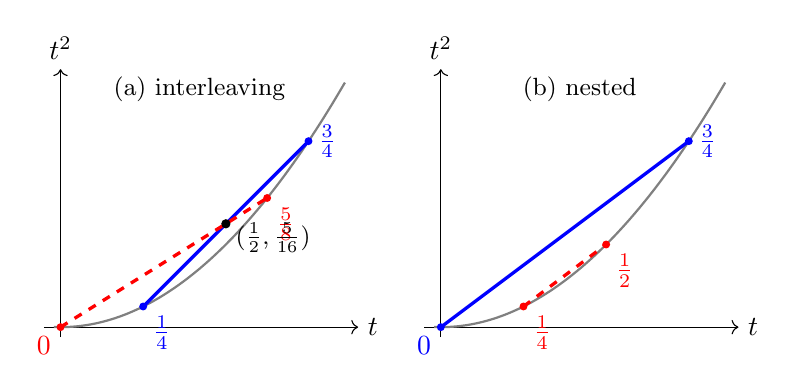
\begin{tikzpicture}[scale=4.2]
\begin{scope}
\draw[->] (-0.05,0) -- (0.9,0) node[right] {$t$};
\draw[->] (0,-0.03) -- (0,0.78) node[above] {$t^2$};
\draw[thick,gray,domain=-0.02:0.86,smooth,variable=\t] plot ({\t},{\t*\t});
\coordinate (a1) at (0.25,0.0625); \coordinate (a2) at (0.75,0.5625);
\coordinate (c1) at (0,0); \coordinate (c2) at (0.625,0.390625);
\draw[very thick,blue] (a1) -- (a2);
\draw[very thick,red,dashed] (c1) -- (c2);
\fill[blue] (a1) circle (0.012) node[below right] {$\tfrac14$};
\fill[blue] (a2) circle (0.012) node[right] {$\tfrac34$};
\fill[red] (c1) circle (0.012) node[below left] {$0$};
\fill[red] (c2) circle (0.012) node[below right] {$\tfrac58$};
\fill (0.5,0.3125) circle (0.014);
\node[anchor=west] at (0.5,0.27) {\small $(\tfrac12,\tfrac5{16})$};
\node at (0.42,0.72) {\small (a) interleaving};
\end{scope}
\begin{scope}[xshift=1.15cm]
\draw[->] (-0.05,0) -- (0.9,0) node[right] {$t$};
\draw[->] (0,-0.03) -- (0,0.78) node[above] {$t^2$};
\draw[thick,gray,domain=-0.02:0.86,smooth,variable=\t] plot ({\t},{\t*\t});
\coordinate (a1) at (0,0); \coordinate (a2) at (0.75,0.5625);
\coordinate (c1) at (0.25,0.0625); \coordinate (c2) at (0.5,0.25);
\draw[very thick,blue] (a1) -- (a2);
\draw[very thick,red,dashed] (c1) -- (c2);
\fill[blue] (a1) circle (0.012) node[below left] {$0$};
\fill[blue] (a2) circle (0.012) node[right] {$\tfrac34$};
\fill[red] (c1) circle (0.012) node[below right] {$\tfrac14$};
\fill[red] (c2) circle (0.012) node[below right] {$\tfrac12$};
\node at (0.42,0.72) {\small (b) nested};
\end{scope}
\end{tikzpicture}
\caption{Moment pairs $(\E y,\E y^2)$ of distributions on a two-point set
form the chord of the parabola between the two points. Solid: $A$;
dashed: $C$. (a) The sets of Proposition~\ref{prop:path-gap} interleave,
the chords cross at $(\tfrac12,\tfrac5{16})$, and the glued pair relaxation
has value $0$. (b) Nested sets: the chords do not meet, and by
Theorem~\ref{thm:interleave} the glued relaxation attains the true minimum
$\delta^2/2$ in the direction of $\Phi$.}
\label{fig:chords}
\end{figure}


Proposition~\ref{prop:path-gap} is the case $[\ell,u]=[0,1]$,
$A=\{\tfrac14,\tfrac34\}$, $C=\{0,\tfrac58\}$ and $\omega_A=\omega_C=1$, with
sorted order $0,\tfrac14,\tfrac58,\tfrac34$. Figure~\ref{fig:chords} shows
what goes wrong. In $R$ the two pairs may represent $y$ by different
distributions that agree only in their first two moments. Each pair places
$y$ on its own preferred two-point set, and whenever the chords cross, the
two distributions have the same mean and second moment. The theorem
concerns the directions $\Phi$ of the family~\eqref{eq:family}; in other
directions on the path the gap can take other values, and
Proposition~\ref{prop:gain}(ii) expresses it for every direction.

\subsection{Matching more moments}\label{sec:k-moments}

The same mechanism defeats any interface that identifies a fixed finite
number of moments of the shared variable. Let $X_L$ and $X_R$ be compact
sets of points $(x,y)$ and $(y,z)$, with $y$ scalar, and let $H_L$ and $H_R$
be the convex hulls of continuous feature maps on them whose first $\kappa$
coordinates are $y,y^2,\dots,y^\kappa$; the other local features are
arbitrary. Let $R_\kappa$ be the set of pairs of points of $H_L$ and $H_R$
that agree in these $\kappa$ coordinates. Let $\Phi_L\ge0$ on $X_L$ and
$\Phi_R\ge0$ on $X_R$ be affine functions of the local features, with zero
sets $Z_L$ and $Z_R$, and let $A$ and $C$ be the projections of $Z_L$ and
$Z_R$ onto $y$. For disjoint compact $A,C\subset\R$, the \emph{alternation
number} $\operatorname{alt}(A,C)$ is the largest $r$ for which there are
points $t_0<\dots<t_r$ of $A\cup C$ with consecutive points in different
sets.

\begin{theorem}[Alternation]\label{thm:alternation}
Suppose $A$ and $C$ are disjoint, so that $\Phi_L+\Phi_R>0$ at every point
$(x,y,z)$ with $(x,y)\in X_L$ and $(y,z)\in X_R$. The linearization of
$\Phi_L+\Phi_R$ vanishes at some point of $R_\kappa$ if and only if
$\operatorname{alt}(A,C)\ge\kappa+1$. In particular, gluing on $\kappa$
moments always gives a positive bound when $\abs A+\abs C\le\kappa+1$, and,
for finite sets with $\abs A+\abs C=\kappa+2$, gives the bound zero exactly
when $A$ and $C$ alternate.
\end{theorem}

\begin{proof}
As in the proof of Theorem~\ref{thm:interleave}, the linearization vanishes
at a point of $R_\kappa$ if and only if there are probability measures on
$A$ and on $C$ with equal moments of orders $1,\dots,\kappa$; these measures
lift to $Z_L$ and $Z_R$ atom by atom. If $\operatorname{alt}(A,C)=r\le\kappa$,
there is a polynomial of degree $r$ that is positive on $A$ and negative on
$C$ (Appendix~\ref{app:alternation}), and its integrals against two such
measures would have to be equal, a contradiction. If
$\operatorname{alt}(A,C)\ge\kappa+1$, take an alternating chain
$t_0<\dots<t_{\kappa+1}$ and the weights $w_i=\prod_{j\ne i}(t_i-t_j)^{-1}$
of the divided difference of order $\kappa+1$. They annihilate all
polynomials of degree at most $\kappa$, and their signs alternate, so their
positive and negative parts, normalized, are probability measures on the
$A$-points and on the $C$-points with equal moments of orders
$0,\dots,\kappa$.
\end{proof}

For finite $A$ and $C$ the criterion is the classical description of Radon
partitions of points on the moment curve: the convex hulls of
$\{(t,\dots,t^\kappa):t\in A\}$ and $\{(t,\dots,t^\kappa):t\in C\}$ meet
exactly when $A$ and $C$ alternate at least $\kappa+1$ times
\citep{Breen1973}. By Gordan's alternative it is equivalent to the fact that
the least degree of a polynomial that is positive on $A$ and negative on $C$
is $\operatorname{alt}(A,C)$, which rests on the sign-change properties of
Chebyshev systems \citep{KarlinStudden1966}. Theorem~\ref{thm:interleave}(ii)
is the case $\kappa=2$. What the theorem adds is its reading as a criterion
for gluing interfaces.

Theorem~\ref{thm:alternation} characterizes when the glued bound is zero,
not when it is exact. For $\kappa\ge3$ the glued bound can lie strictly
between $0$ and the minimum. For $\Phi_L=(y-2x)^2+4x(1-x)$ and
$\Phi_R=(y-1-2z)^2+4z(1-z)$ with $x,z\in[0,1]$ and $y\in[0,3]$ we have
$A=\{0,2\}$, $C=\{1,3\}$ and $\operatorname{alt}(A,C)=3$, so gluing on
$\kappa=3$ moments gives a positive bound. The probability measures
\[
\nu_A=\tfrac{57}{112}\,\delta_{15/32}+\tfrac{55}{112}\,\delta_{57/32},\qquad
\nu_C=\tfrac{22}{117}\,\delta_{0}+\tfrac{1045}{1456}\,\delta_{39/32}+\tfrac{95}{1008}\,\delta_{81/32}
\]
on $[0,3]$ have equal moments of orders up to three, and
$\int\dist(y,A)^2d\nu_A+\int\dist(y,C)^2d\nu_C=6103/16128\approx0.378$,
whereas $\min(\Phi_L+\Phi_R)=1/2$. The dichotomy of
Theorem~\ref{thm:interleave} is therefore specific to two shared moments and
two-point sets. Every $\kappa$ is nevertheless defeated by some quadratic
configuration.

\begin{proposition}[A full gap for every $\kappa$]\label{prop:full-gap}
Let $\kappa\ge1$ and choose $r\ge1$ with $\kappa\le2^{r+1}-2$. On
$x,z\in[0,1]^r$ and $y\in[0,2^{r+1}-1]$ let
\[
\Phi_L=\Bigl(y-\sum_{j=1}^r2^jx_j\Bigr)^2+\sum_{j=1}^r4^jx_j(1-x_j),\qquad
\Phi_R=\Bigl(y-1-\sum_{j=1}^r2^jz_j\Bigr)^2+\sum_{j=1}^r4^jz_j(1-z_j).
\]
Let $H_L$ be the convex hull of the features $y,\dots,y^{\max\{\kappa,2\}}$,
$x_j$, $yx_j$ and $x_ix_j$ $(i<j)$ over $[0,1]^r\times[0,2^{r+1}-1]$, and $H_R$
the analogous hull in $(y,z)$. Then $\min(\Phi_L+\Phi_R)=1/2$, while the
linearization of $\Phi_L+\Phi_R$ vanishes at a point of $R_\kappa$.
\end{proposition}

\begin{proof}
The coefficient of $x_j^2$ in $\Phi_L$ is $4^j-4^j=0$, so $\Phi_L$ is affine
in the features and multilinear in $x$. Its minimum over $x$ is therefore
attained at a vertex, where it equals $(y-\sum_{j\in J}2^j)^2$ for a subset
$J$; hence $\min_x\Phi_L=\dist(y,A)^2$ with $A=\{0,2,\dots,2^{r+1}-2\}$, and
similarly $\min_z\Phi_R=\dist(y,C)^2$ with $C=\{1,3,\dots,2^{r+1}-1\}$. By the
argument of Theorem~\ref{thm:interleave}(i), with $\delta=1$, the minimum is
$1/2$. The points $0,1,\dots,\kappa+1$ alternate between $A$ and $C$, so
Theorem~\ref{thm:alternation} applies; explicitly, the binomial weights
$\binom{\kappa+1}i2^{-\kappa}$ on the even and on the odd integers
$i\le\kappa+1$ have equal moments of orders up to $\kappa$.
\end{proof}

Thus no fixed number of shared moments makes the gluing exact, even for
quadratic blocks, and the relative gap can be $100\%$. As $\kappa\to\infty$
the glued bounds do converge to the true minimum, because measures on a
compact interval are determined by their moments and measures with equal
marginals glue \citep[Lemma~6.3]{Lasserre2006}; the convergence is not
uniform over instances.

\subsection{Relation to known results}\label{sec:composition-literature}

Several earlier examples show that sparse relaxations on a path can be
strictly weaker than dense ones. \citet[Example~3.5]{NieDemmel2009} give a
numerical quartic example, and \citet[Example~6.7]{NieQuTangZhang2026} a
box-constrained quartic for which the sparse moment hierarchy is never
tight. Finite gluing results require rank or flatness conditions on the
overlaps \citep[Theorem~3.7]{Lasserre2006}, \citep{FantuzziFuentes2025}.
For quadratic problems with sign-oriented squares,
\citet[Corollary~1]{DeyKhajavirad2025} decompose the convex hull across a
complete separator that carries no positive square term (no ``plus loop''),
and \citet{Khajavirad2026} builds on this decomposition.
Proposition~\ref{prop:path-gap} shows that the hypothesis cannot be dropped
even for a path of three variables with a single plus loop at the center:
the reduced objective
$2y^2-\tfrac12y-xy-\tfrac54yz+\tfrac1{16}+\tfrac12x+\tfrac{25}{64}z$, which
equals $\Phi$ at binary leaves, has the same witness and the same gap $1/128$.
Their stable-set theorem \citep[Theorem~2]{DeyKhajavirad2025} still gives an
exact extended formulation for this sign pattern, because the plus-loop node
$y$ is a stable set, but it adds the products among the neighbors of $y$,
here the nonedge product $xz$; this matches the next paragraph. To our
knowledge, a degree-two example with exact pair hulls, an exact rational gap
and a separating cut in the existing coordinates, the value $\delta^2/2$ of
the gap in Theorem~\ref{thm:interleave}, and the use of the alternation
criterion to decide when a $\kappa$-moment interface gives no positive bound
have not been given before.

The advantage of the joint block over its pairs does not extend to dense
relaxations. Sparse and dense Shor relaxations \citep{Shor1987} coincide
for chordal sparsity patterns, because a partial positive semidefinite
matrix with a chordal pattern has a positive semidefinite completion
\citep{GroneEtAl1984,WakiEtAl2006,Laurent2009}. Hence $R$ is the projection of
the dense moment relaxation of $(1,x,y,z)$ with the RLT inequalities
\citep{SheraliAdams1990,SheraliTuncbilek1992} of the edges and squares, and
what closes the gap must come from the RLT inequalities of the nonedge
product $xz$. On the whole family~\eqref{eq:family}, with
$\xi_A=y-a_1-(a_2-a_1)x$ and $\xi_C=y-c_1-(c_2-c_1)z$,
\begin{equation}\label{eq:sdp-identity}
\Phi-\frac{\delta^2}2=\frac{(\xi_A+\xi_C)^2}2+\sum_{i,j\in\{0,1\}}F_{ij}\,\ell_{ij}(x,z)
+\Bigl(\omega_A-\frac{(a_2-a_1)^2}2\Bigr)x(1-x)+\Bigl(\omega_C-\frac{(c_2-c_1)^2}2\Bigr)z(1-z),
\end{equation}
where $\ell_{00}=(1-x)(1-z)$, $\ell_{10}=x(1-z)$, $\ell_{01}=(1-x)z$,
$\ell_{11}=xz$, and $F_{ij}=\tfrac12\bigl((c_{j+1}-a_{i+1})^2-\delta^2\bigr)\ge0$.
The linearized $\ell_{ij}$ are the McCormick expressions of the product $xz$,
the linearized $(\xi_A+\xi_C)^2$ is a quadratic form in the dense moment matrix
of $(1,x,y,z)$, and the last two terms are nonnegative on the pair hulls.
Hence the dense moment matrix together with the McCormick inequalities of
the nonedge product $xz$ proves $\Phi\ge\delta^2/2$ for every member of the
family, and neither ingredient alone suffices (Appendix~\ref{app:sdp}). This
is a special case of a theorem of \citet[Theorem~1]{BurerNatarajanWillemsen2025}:
for box-constrained quadratic programs in at most three variables whose
off-diagonal coefficients are nonpositive, the Shor relaxation with the RLT
upper bounds is exact. On a path $x$--$y$--$z$ over a box, replacing $x$ by
its complement or $z$ by its complement where necessary makes the
coefficients of $xy$ and $yz$ nonpositive, the coefficient of $xz$ stays zero,
and complementation maps McCormick inequalities to McCormick inequalities.
The dense moment relaxation with the McCormick inequalities of all products,
including $xz$, is therefore exact for every quadratic objective on a
three-variable path over a box, and~\eqref{eq:sdp-identity} is an explicit
certificate for the family. The support inequality~\eqref{eq:path-cut}
attains the same bound without the coordinate $p_{xz}$ and without a
semidefinite constraint. That matters in practice, because solvers relax the
products present in the model and rarely add new ones; but the advantage is
one of representation, not of strength over such relaxations.

\subsection{When gluing is exact, and the gain from merging}\label{sec:gluing}

Gluing is exact when the shared coordinates determine the shared
distribution. Under a running-intersection decomposition, local measures
with equal full marginals on the separators glue to a global measure
\citep{Vorobev1962,Lasserre2006}, and \citet[Corollary~3.10]{Tawarmalani2010}
glues two functions that share a variable when their inclusion certificates
have equal marginals of that variable. If the separator takes finitely many
known values $t_1,\dots,t_N$, its moments of orders $0,\dots,N-1$ determine
its distribution through a Vandermonde system; for a binary separator the
mean suffices. This is why the McCormick inequalities describe the convex
hull of a pure bilinear function on a forest over the unit box
\citep[Proposition~8]{Padberg1989}: the extreme points are binary, the
McCormick inequalities of an edge are the nonnegativity of the four joint
probabilities of its endpoints, and adjacent edges share a binary variable
whose distribution is fixed by its mean. Square terms break this argument,
because they let a fractional mean be realized by continuous distributions,
as in~\eqref{eq:witness}.

The gain from merging pair directions into one star direction can be
computed exactly, and it is related to the glued relaxation by a
re-splitting of the center terms.

\begin{proposition}[Gain from merging]\label{prop:gain}
Let $P_i\subset\R^2$ be rational polytopes in the variables $(y,x_i)$,
$i=1,\dots,k$, whose star domain $\Omega=\{(y,x):(y,x_i)\in P_i\text{ for all }i\}$
is nonempty, and let $q_i(y,x_i)$ be rational quadratics. Put
$\beta_i=\min_{P_i}q_i$, $\beta^\ast=\min_\Omega\sum_iq_i$ and
$\Delta=\beta^\ast-\sum_i\beta_i$.
\begin{enumerate}[label=(\roman*)]
\item $\Delta\ge0$ is the largest constant $c$ such that
$\sum_iq_i\ge\sum_i\beta_i+c$ on $\Omega$, and $\Delta>0$ if and only if the
projections onto $y$ of the sets $\argmin_{P_i}q_i$ have empty common
intersection.
\item Let $R_\Omega$ be the set of $k$-tuples of points of the pair hulls
$\conv\{(y,x_i,y^2,yx_i,x_i^2):(y,x_i)\in P_i\}$ that agree in $(m_y,s_y)$.
Then $\beta^\ast-\min_{R_\Omega}\sum_i\operatorname{lin}q_i=\inf\Delta'$, where
the infimum is over all re-splittings $q_i'=q_i+\alpha_iy+\gamma_iy^2$ with
$\sum_i\alpha_i=\sum_i\gamma_i=0$, and $\Delta'$ is computed as $\Delta$ for
the $q_i'$.
\end{enumerate}
\end{proposition}

\begin{proof}
(i) Clearly $\sum_iq_i\ge\sum_i\beta_i$ on $\Omega$, and $\beta^\ast$ is the
best constant in that direction. If some $\bar y$ lies in every projection,
choose $x_i$ with $(\bar y,x_i)\in\argmin_{P_i}q_i$; the assembled point lies
in $\Omega$ and attains $\sum_i\beta_i$. Conversely, if $\Delta=0$, a minimizer
over $\Omega$ minimizes every $q_i$, so its $y$-coordinate lies in every
projection.

(ii) A re-splitting does not change $\sum_iq_i$, so $\beta^\ast$ is the same for
all of them. The set $R_\Omega$ is the intersection of the compact convex
product of the pair hulls with the linear equations
$m_y^{(i)}=m_y^{(1)}$ and $s_y^{(i)}=s_y^{(1)}$ for $i\ge2$, and it is
nonempty because $\Omega$ is. Attach multipliers to these equations. Their
Lagrangian is bilinear, and by the minimax theorem for a compact convex
set \citep{Sion1958} the minimum of $\sum_i\operatorname{lin}q_i$ over
$R_\Omega$ equals the supremum over the multipliers of the minimum of the
Lagrangian over the product of the pair hulls. A choice of multipliers is
exactly a re-splitting with $\sum_i\alpha_i=\sum_i\gamma_i=0$, and the minimum
of the Lagrangian then separates into $\sum_i\min_{P_i}q_i'=\sum_i\beta_i'$.
Hence $\min_{R_\Omega}\sum_i\operatorname{lin}q_i=\sup\sum_i\beta'_i$, which is
the claim.
\end{proof}

Both $\beta_i$ and $\beta^\ast$ are computed exactly by the algorithms of
Section~\ref{sec:quadratic}; in Proposition~\ref{prop:path-gap} both pair
minima are zero and $\Delta=1/128$. Since each $\beta_i'$ is a minimum of
functions that are affine in $(\alpha_i,\gamma_i)$, part~(ii) turns the gap of
the glued relaxation in any direction into the maximization of a concave
function of $2(k-1)$ parameters whose oracle is the pair minimum. The quantity $\Delta$ compares the merged
cut with separately added pair cuts for one decomposition, and the gap to
the glued relaxation is its infimum over re-splittings. For example, with
$q_1=\Phi_A$ and $q_2=\Phi_C$ for the nested sets $A=\{0,3\}$ and $C=\{1,2\}$
on $y\in[0,3]$, both pair minima are zero and $\Delta=\beta^\ast=1/2$; the
re-splitting $q_1+\tfrac12(y-\tfrac32)^2$ and $q_2-\tfrac12(y-\tfrac32)^2$ has
pair minima $\tfrac34$ and $-\tfrac14$, so $\Delta'=0$, in agreement with the
zero gap of Theorem~\ref{thm:interleave}. The polynomials $p$ of
Appendix~\ref{app:interleave} are optimal re-splittings of this kind.
Pairwise intersections of the projections in (i) do not suffice when
$k\ge3$: for three leaves of the form $\Phi_A$ with $A_1=\{0,1\}$,
$A_2=\{1,2\}$ and $A_3=\{0,2\}$ on $y\in[0,2]$, the projections meet pairwise
but have no common point, and $\Delta=2/3$. The proposition is a diagnostic
for a proposed merge; it does not say which directions to merge or whether
merging pays off in a solver.

\section{Exact support for quadratic blocks}\label{sec:quadratic}

If every feature $f_j$ is a quadratic polynomial, then every support
problem~\eqref{eq:support} asks for the minimum of a single quadratic
function over the block domain. This section gives two exact rational
algorithms for that problem. The first works for any bounded polytope of
small dimension; the second works for quadratic stars of any size whose
constraints couple the center with one leaf at a time. Both return an
attained minimizer and a rational minimum, so they serve as exact support
oracles and give support inequalities that are tight.

\subsection{Bounded polytopes in fixed dimension}\label{sec:polytope}

Let $P=\{x\in\R^d:Ax\le b\}$ be a bounded polytope given by $m$ rational
rows, which include finite variable bounds, and let
$q(x)=\tfrac12x\T Hx+c\T x+c_0$ with rational data and $H=H\T$. The matrix
$H$ may be indefinite or singular, $P$ may be lower-dimensional, and rows
may be redundant or implied equalities; an equality is given by two
opposite rows. For a set $I$ of rows, $A_I$ and $b_I$ denote the
corresponding submatrix and subvector, and
\begin{equation}\label{eq:kkt-system}
M_I=\begin{pmatrix}H&A_I\T\\ A_I&0\end{pmatrix},\qquad
M_I\begin{pmatrix}x\\ \mu\end{pmatrix}=\begin{pmatrix}-c\\ b_I\end{pmatrix}.
\end{equation}
The \emph{candidates} are the points $x$ obtained from all sets $I$ with
$\abs I\le d$ for which $M_I$ is nonsingular and $Ax\le b$ holds. The
multipliers $\mu$ are not sign-restricted: the system expresses
stationarity on the affine hull of a face, not a KKT condition.

\begin{theorem}[Exact quadratic support on a polytope]\label{thm:polytope}
If $P\ne\emptyset$, some candidate minimizes $q$ over $P$; hence the least
candidate value is $\min_Pq$, and it is attained at a rational point. If
there is no candidate, then $P=\emptyset$. Both statements remain true if
only sets $I$ of linearly independent rows are enumerated.
\end{theorem}

The proof (Appendix~\ref{app:polytope}) chooses a global minimizer in the
relative interior of a face of smallest dimension and shows that $H$ is
positive definite on the face's direction space, so that a nonsingular
system~\eqref{eq:kkt-system} of independent active rows has this minimizer
as its solution. The sign of the multipliers and the inertia of $H$ need not
be tested, because extra candidates, such as saddle points of faces, are
feasible and cannot produce a value below the minimum. Dependent rows never
give a nonsingular $M_I$, so duplicate, redundant and opposite rows are
harmless. Two parts of the argument cannot be dropped. Boundedness is needed:
for $P=\{x\in\R:x\ge0\}$ and $q=-x$ the enumeration returns $0$, and for
$P=\R$ and $q=x$ it returns no candidate. The choice of a minimizer on a face
of minimal dimension is also needed: for $q=(x-y)^2$ on $[0,1]^2$, the
minimizers $(t,t)$ with $0<t<1$ give only singular systems, and the
enumeration finds the minimizers $(0,0)$ and $(1,1)$ instead.

\begin{corollary}[Support of a quadratic feature graph]\label{cor:quad-features}
If $f_1,\dots,f_p$ are quadratic polynomials with rational coefficients and
$(a,b)$ is rational, the support value $h_P(a,b)$ is the rational number
obtained by applying Theorem~\ref{thm:polytope} to $q=a\T x+b\T F$, and the
support inequality is tight at the returned minimizer.
\end{corollary}

There are at most $N(m,d)=\sum_{j=0}^d\binom mj$ sets $I$. For each,
Gaussian elimination on a system of order at most $2d$ and the feasibility
test take $O(d^3+md)$ arithmetic operations, so the enumeration uses
$O(N(m,d)(d^3+md))$ operations. With fraction-free elimination, every
intermediate number is a minor of an integer matrix of order at most $2d$,
and Hadamard's inequality bounds the bit length of every candidate and of
the minimum by $O(d(\langle q\rangle+\langle A\rangle+\log d))$, where
$\langle q\rangle$ is the encoding length of $q$ and $\langle A\rangle$ the
largest encoding length of a row (Appendix~\ref{app:polytope}). For fixed
$d$ the algorithm is therefore strongly polynomial, and the minimum has
polynomial encoding length, in line with the result that quadratic
programming is in NP \citep{Vavasis1990}. The method is total enumeration of
faces \citep[Section~2.9]{Murty1997}; what we add is the treatment of the
degenerate cases that a certificate must cover.

Without a bound on the dimension the problem is hard. The following facts
are folklore \citep[Section~2.3]{BurerLetchford2009}; Appendix~\ref{app:polytope}
gives the short proofs.

\begin{proposition}[Hardness in unrestricted dimension]\label{prop:maxcut}
Computing $\min_{x\in[0,1]^n}q(x)$ for rational quadratics $q$ is strongly
NP-hard, even when $q$ is multilinear with integer coefficients of absolute
value at most $n$. Deciding whether a given inequality $q(x)\ge t$ holds on
$[0,1]^n$ is coNP-complete.
\end{proposition}

Unless NP${}={}$coNP, the validity of an exact support cut for a quadratic
block of unrestricted size therefore has no short certificate that can be
checked in polynomial time, and a certificate that is replayed by repeating
the enumeration, as ours is, is natural for this class. Useful exact oracles
must restrict the dimension, as in Theorem~\ref{thm:polytope}, or the
structure, as in the next subsection. Restricting the interaction graph alone
is not enough: box-constrained quadratic minimization is strongly NP-hard
already at treewidth two, and quartic minimization already on paths
\citep[Theorems~2 and~3]{DelPiaKhajavirad2026}.

\subsection{Quadratic stars with center--leaf constraints}\label{sec:star}

Section~\ref{sec:composition} shows that the blocks worth merging are often
stars: several pairs that share one variable. For stars there is an exact
algorithm whose cost is nearly linear in the size of the block. Let $y$ be
the center and $x_1,\dots,x_k$ the leaves, and consider
\begin{equation}\label{eq:star}
q(y,x)=c_0+c_1y+c_2y^2+\sum_{i=1}^k\bigl(\alpha_ix_i^2+(\beta_iy+\gamma_i)x_i\bigr)
\end{equation}
with rational coefficients of arbitrary signs. The domain $\Omega$ is given by
finite rational bounds on all variables and by rational affine rows, each of
which involves $y$ and \emph{at most one} leaf; an equality is given as two
rows. Every scalarization $a\T(y,x)+b\T F(y,x)$ of a vector $F$ of quadratics
with this interaction pattern has the form~\eqref{eq:star}. Rows that couple
two leaves are excluded, because with them the problem is NP-hard already
without a center: $\min\sum_ix_i(1-x_i)$ over $0\le x\le1$ and
$\sum_ia_ix_i=b$ is zero exactly when the subset-sum instance $(a,b)$ is
feasible \citep{Karp1972}; compare \citet{MoreVavasis1990}.

For fixed $y$, the rows of leaf $i$ restrict $x_i$ to an interval
$[L_i(y),U_i(y)]$, where $L_i$ is the maximum of the affine lower bounds and
$U_i$ the minimum of the affine upper bounds that these rows and the leaf
bounds define. Thus $L_i$ is convex and $U_i$ concave, both piecewise
affine. The set $J_i=\{y:L_i(y)\le U_i(y)\}$ is an interval because $L_i-U_i$
is convex. Given $y$, the leaves are constrained independently, so the
projection of $\Omega$ onto $y$ is the interval $I$ obtained by intersecting
the bounds of $y$, the rows in $y$ alone, and all $J_i$. If $I$ is empty, so
is $\Omega$.

\begin{theorem}[Exact support on constrained stars]\label{thm:star}
Let $m$ be the number of rows that involve a leaf and $m_0$ the number of
rows in $y$ alone, and suppose $\Omega$ is nonempty. Then $\min_\Omega q$ is
attained at a rational point, and it can be computed, together with a
minimizer and a partition of $I$ into at most $2m+4k+1$ intervals on each of
which every leaf has an affine minimizer, with $O(m_0+(m+k)\log(m+k))$
arithmetic operations and comparisons. All numbers involved have bit length
polynomial in the input length; the breakpoints have bit length bounded
independently of $k$.
\end{theorem}

\begin{proof}
Define $\varphi_i(y)=\min\{\alpha_ix_i^2+(\beta_iy+\gamma_i)x_i:L_i(y)\le x_i\le U_i(y)\}$
for $y\in I$, so that $\min_\Omega q=\min_{y\in I}V(y)$ with
$V(y)=c_0+c_1y+c_2y^2+\sum_i\varphi_i(y)$. Let $s_i=m_i+2$ be the number of
affine functions that define $L_i$ and $U_i$, where $m_i$ is the number of
rows of leaf $i$; together $L_i$ and $U_i$ have at most $s_i-2$ breakpoints.

If $\alpha_i>0$, the minimizer is $\xi_i=\max\{L_i,\min\{v_i,U_i\}\}$ with
the affine function $v_i(y)=-(\beta_iy+\gamma_i)/(2\alpha_i)$. The function
$v_i-L_i$ is concave and $v_i-U_i$ convex, so each has at most two isolated
zeros, and $\xi_i$ is affine between consecutive points of a set of at most
$s_i+2$ breakpoints. If $\alpha_i\le0$, a minimizer is an endpoint of the
interval, and
\begin{equation}\label{eq:endpoint-factor}
\psi_i(U_i)-\psi_i(L_i)=(U_i-L_i)\bigl(\alpha_i(U_i+L_i)+\beta_iy+\gamma_i\bigr),
\qquad\psi_i(t)=\alpha_it^2+(\beta_iy+\gamma_i)t .
\end{equation}
The first factor is nonnegative on $I$. On each of the at most $s_i-1$
intervals where $L_i$ and $U_i$ are affine, the second factor is affine and
has at most one zero, which decides the preferred endpoint; this gives at
most $2s_i-3$ breakpoints. Taking all breakpoints together splits $I$ into at
most $\sum_i2s_i+1=2m+4k+1$ intervals on which every leaf rule is affine and
$V(y)=q(y,\xi(y))$ is a quadratic polynomial in $y$.

Each $\varphi_i$ is continuous on $I$, since it is the minimum of a continuous
function over an interval whose endpoints depend continuously on $y$. Hence
$V$ agrees with the quadratic of each interval on its closure, and the
minimum of $V$ is the least value of these quadratics at the interval
endpoints and, where the leading coefficient is positive, at interior
stationary points. All breakpoints and all endpoints of $I$ are zeros of
affine functions with rational coefficients, so every candidate is rational,
and the minimizing $y$ together with $x_i=\xi_i(y)$ is a rational minimizer.

For the operation count, intersecting the bounds of $y$ with the $m_0$ rows
in $y$ alone costs $O(m_0)$. The upper envelope of $s_i$ lines is computed by
sorting slopes and one stack-based scan in $O(s_i\log s_i)$ operations, and
$J_i$, the breakpoints and the rules of leaf $i$ in $O(s_i)$ more. Sorting all
breakpoints costs $O((m+k)\log(m+k))$. A sweep over the sorted breakpoints
maintains the three coefficients of $V$; at each breakpoint only the leaves
whose rule changes are updated, so the sweep takes $O(m+k)$ operations. Bit
lengths are bounded in Appendix~\ref{app:star}.
\end{proof}

The bound on the number of intervals is tight up to a constant factor: a
single concave leaf whose bounds zigzag forces $2s_i-3$ rule changes, and $k$
hinge leaves force $k$ more, so the partition can need $\Theta(m+k)$
intervals. On instances with $m=\Theta(k)$, the operation bound is optimal up
to a constant factor for algebraic computation trees: by Ben-Or's theorem,
applied to a family of instances with $3r$ leaves and $r$ rows whose decision
set has $r!$ connected components, deciding whether the minimum is at least a
given value requires $\Omega((m+k)\log(m+k))$ operations
(Appendix~\ref{app:star}).

\paragraph{Relation to forest algorithms.}
\citet{DelPiaKhajavirad2026} solve box-constrained quadratic programs on
forests with $O(n^2)$ arithmetic operations. After an affine scaling of each
variable to $[0,1]$, a box-constrained star is such a forest, and their
dynamic program rooted at the center specializes to the box-constrained case
of Theorem~\ref{thm:star}; in that case our contribution is only the
$O(k\log k)$ count, which replaces their $O(k^2)$ merge at the root. Rows
that couple the center with a leaf are outside their model. A shear
$x_i\mapsto x_i-\rho y$ turns a leaf domain that is a parallelogram with two
vertical sides back into a box and keeps the star structure, but triangles,
trapezoids with nonparallel sides and polygons with more sides cannot be
reduced in this way. Such rows also break the structural property on which
their algorithm rests: the conditional value of a leaf is then no longer a
minimum of affine functions of $y$ over a fixed set, and it can have convex
kinks. For example, for $x\in[0,1]$ with rows $x\ge y-\tfrac12$ and
$x\ge\tfrac12-y$, the minimum of $x$ is $\abs{y-\tfrac12}$. The SOC
descriptions of star hulls by \citet{DeyKhajavirad2025} assume sign patterns
of the square terms and box domains, and the LP approximations of
\citet{BienstockMunoz2018} allow constraints but are approximate. Our
algorithm conditions on the center, as nonserial dynamic programming does
\citep{BerteleBrioschi1972}, and solves a one-parameter quadratic problem for
each leaf, a special case of multiparametric quadratic programming
\citep{Bemporad2002}; \citet{BhathenaEtAl2025} use parametric dynamic
programs of this kind on trees for convex quadratic problems with
indicators. To our knowledge, no exact algorithm for nonconvex stars with
center--leaf rows has been published.

\begin{remark}[Deeper trees]\label{rem:trees}
The argument uses that every vertex other than the center is a leaf. On the
path $x_1$--$x_2$--$x_3$ over $[0,1]^3$ with
$f=(x_2-\tfrac18)x_1+x_2^2-x_2+x_2x_3+x_3^2-x_3$, the conditional value of the
subtree $\{x_1,x_2\}$ given $x_3=t$ is
$\min\{-\tfrac18,\,-\tfrac14(1-t)^2\}$, which switches at the irrational point
$t=1-\sqrt2/2$, although $\min f=-\tfrac38$ is rational
(Appendix~\ref{app:star}). Rooted at $x_2$, the same path is a star, and
Theorem~\ref{thm:star} gives a rational partition; the obstruction concerns
nesting conditional values along a tree of depth two.
\citeauthor{DelPiaKhajavirad2026} handle such breakpoints for boxes with an
explicit algebraic representation; we do not know whether edge-local affine
rows can be added to deeper trees with a polynomial algorithm.
\end{remark}

The certificate of a star support value records the partition of $I$, the
affine rule of every leaf on every piece, the quadratic of $V$ on every piece
and the candidates; a checker rebuilds the partition from the rows and
coefficients and compares. The star oracle in our implementation is simpler
than the algorithm of the proof: it splits the center interval at all
pairwise intersections of each leaf's bound lines and recomputes every leaf
rule on every piece. This costs $O((m+k)^3)$ operations, stores $\Theta(k)$
rules per piece, and can produce more pieces than Theorem~\ref{thm:star}
requires. It certified the star cuts of our first implementation, whose
stars had at most four leaves (Appendix~\ref{app:campaigns12}); in the
experiments of Section~\ref{sec:computations} every block had at most four
variables, and the polytope oracle certified every quadratic cut.
Section~\ref{sec:star-bench} compares the two star algorithms on random
stars with up to $10^4$ leaves.

\section{Cuts in the original variables}\label{sec:original}

Proposition~\ref{prop:support} produces inequalities in lifted coordinates
$(x,w)$. Using them requires variables $w_j$ with $w_j=f_j(x)$ in the model.
If the solver's representation does not already contain exactly these
variables, adding them changes the model: new equalities, new variables for
branching and propagation, and possibly a different presolve. Our first
implementation used such a reformulation and needed a control mode to
separate its effect from that of the cuts (Appendix~\ref{app:campaigns12}).
This section shows how to avoid the auxiliary variables. The nonlinear
functions are minimized jointly over the block domain, and the rows of the
model then eliminate them. The underlying facts are classical Lagrangian
duality; we state them in the form that the implementation and its
certificates need.

\subsection{Aggregating nonlinear rows}\label{sec:aggregation}

Let $v\in\R^N$ be the vector of all model variables, including an objective
variable if there is one, and let $x=Sv$ be a block of $n$ of them, selected
by a $0/1$ matrix $S$. Suppose the model contains rows
\begin{equation}\label{eq:rows}
g(Sv)+Av\le b
\end{equation}
with $g:D\to\R^m$ and affine remainders $Av$ that may involve any variables,
including block variables; an equality is written as two opposite rows. Here
$D$ is a compact set that contains the block part $Sv$ of every point to
which the cuts must apply, for example the block box intersected with the
affine rows that involve only block variables.

\begin{proposition}[Aggregated support cut]\label{prop:aggregate}
Let $a\in\R^n$, $\lambda\in\R^m_{\ge0}$ and
\begin{equation}\label{eq:agg-support}
\beta\ \le\ \varphi(a,\lambda):=\inf_{u\in D}\bigl\{a\T u+\lambda\T g(u)\bigr\}.
\end{equation}
Then every point that satisfies~\eqref{eq:rows} and $Sv\in D$ satisfies
\begin{equation}\label{eq:agg-cut}
(S\T a-A\T\lambda)\T v\ \ge\ \beta-\lambda\T b .
\end{equation}
\end{proposition}

\begin{proof}
At such a point, $\lambda\ge0$ gives $\lambda\T g(Sv)\le\lambda\T(b-Av)$.
Substitute this into $a\T Sv+\lambda\T g(Sv)\ge\beta$.
\end{proof}

This is weak Lagrangian duality
\citep[Sections~5.1.3 and~5.2.2]{BoydVandenberghe2004}. It needs neither
convexity nor optimal multipliers. The same inequality is the Lagrangian
cut of a block in the extended block-separable reformulation of
\citet[Section~7.1]{Nowak2005}, after the block's auxiliary variables are
eliminated with the rows~\eqref{eq:rows}; related cuts and range reductions
appear in \citet{TawarmalaniSahinidis2004}, \citet{KaruppiahGrossmann2008}
and \citet{DomesNeumaier2016}. Its strength comes from minimizing the
nonlinear functions jointly over their common domain before they are
eliminated. Nonnegative combinations of linear rows that are already in the
relaxation cannot cut off any point of it.

An objective is handled through its epigraph. For minimization of
$g_0(x)+\ell_0(v)+c_0$ with objective variable $t$, the row
$g_0(x)+\ell_0(v)-t\le-c_0$ is one of the rows~\eqref{eq:rows}; for
maximization the hypograph row $-g_0(x)-\ell_0(v)+t\le c_0$ is used. The two
multipliers of the rows of an equality may be combined into one free
multiplier. Validity uses only $Sv\in D$ and the selected rows. Integrality,
the other constraints and the objective play no role, so the cut is valid
for the mixed-integer feasible set and for its closed convex hull. If $D$ is
built from bounds valid only at a node of the search tree, or from an
incumbent cutoff, the cut is valid only there; our implementation uses only
original bounds and rows, so its cuts are global.

The choice of $D$ matters: affine rows that involve only block variables
belong in $D$, not only in the LP. On the triangle $\{(x,y):x,y\ge0,\ x+y\le1\}$
every point satisfies $x^2+2xy+y^2\le x+y$ and $xy\le\tfrac14$, because
$s=x+y\in[0,1]$ gives $s^2\le s$ and $4xy\le s^2$. In the coordinates
$(m_x,m_y,s_x,s_y,p_{xy})$ these are linear inequalities valid for the hull
of the quadratic graph over the triangle. The point
$(\tfrac12,\tfrac12,\tfrac12,\tfrac12,\tfrac12)$, the average of the graph points
at $(0,0)$ and $(1,1)$ of the box $[0,1]^2$, lies in the hull over the box and
satisfies $m_x+m_y\le1$, but violates both inequalities. Intersecting the
hull over the box with the row is therefore strictly weaker than
convexifying over the row-constrained domain, as is known for factorable
relaxations \citep{Anstreicher2012,ZhuHeTawarmalani2026,WuMutsNowakHendrix2025}.
Here the first inequality is the sum of the RLT products $(1-x-y)x\ge0$ and
$(1-x-y)y\ge0$, so the example shows the weakness of the box hull, not an
advantage over RLT or semidefinite relaxations; for a single bilinear term,
SCIP's projection-based envelopes \citep{MullerSerranoGleixner2020} exploit
linear rows in the same spirit.

\subsection{What the cuts can express}\label{sec:closure}

Let $K=\conv\{(u,g(u)):u\in D\}$ and $Q=\{0\}\times\R^m_{\ge0}$. The affine
map $T(v)=(Sv,\ b-Av)$ places a model point in the lifted space of the block.
The next theorem identifies the set described by all cuts~\eqref{eq:agg-cut}.
It is the set version of the classical fact that the Lagrangian dual bound of
a nonconvex problem equals the optimal value of its convexification in the
joint space of variables and constraint values
\citep{Falk1969,Geoffrion1974,FeltenmarkKiwiel2000,LemarechalRenaud2001}; the
separation argument is the one that \citet[Theorem~3]{ChenLuedtke2022} use
for Lagrangian cuts in two-stage integer programs. We include the short proof
because our setting has nonlinear rows and affine remainders on arbitrary
variables, and because no constraint qualification is needed.

\begin{theorem}[Closure of the aggregated cuts]\label{thm:closure}
Let $D\subset\R^n$ be nonempty and compact and let $g$ be continuous on $D$.
A point $v$ satisfies every inequality~\eqref{eq:agg-cut} with
$\beta=\varphi(a,\lambda)$, over all $a\in\R^n$ and $\lambda\in\R^m_{\ge0}$, if
and only if
\begin{equation}\label{eq:closure}
v\in\mathcal C:=T^{-1}(K+Q)=\bigl\{v:\ \exists\,y\ \text{with}\ (Sv,y)\in K\ \text{and}\ y\le b-Av\bigr\}.
\end{equation}
\end{theorem}

\begin{proof}
The set $K$ is compact and convex, and $Q$ is a closed convex cone, so
$U=K+Q$ is closed and convex. A linear functional $(a,\lambda)$ has finite
infimum on $U$ only if $\lambda\ge0$, and then the infimum is
$\varphi(a,\lambda)$. Evaluating the valid inequality
$a\T u+\lambda\T y\ge\varphi(a,\lambda)$ of $U$ at $T(v)$ gives
exactly~\eqref{eq:agg-cut}, so every point of $\mathcal C$ satisfies all cuts.
Conversely, if $T(v)\notin U$, a linear functional strictly separates $T(v)$
from $U$; its infimum on $U$ is finite, so $\lambda\ge0$, and the
corresponding cut is violated at $v$.
\end{proof}

If auxiliary variables $w=g(x)$ were added, the joint-graph relaxation of the
block would be $(x,w)\in K$, $w+Av\le b$, and its projection onto $v$ is
$\mathcal C$. The direct cuts can therefore express exactly what this lifted
relaxation expresses about the original variables, without adding variables
or equalities to the model, and no more. Relaxations that keep the rows
inside the block, such as the convex-hull relaxations of block-decomposition
methods \citep[Section~3]{Nowak2005}, \citep{WuMutsNowakHendrix2025}, can be
strictly stronger (Example~\ref{ex:quarter}). There is also a cost: with the
same linearization points, outer approximation of a lifted formulation can be
tighter than outer approximation in the original space
\citep{TawarmalaniSahinidis2005}, and a finite set of direct cuts may need
more members than a lifted description. For one row, $\mathcal C$ is the
familiar envelope relaxation. Write $\operatorname{vex}g$ and
$\operatorname{cav}g$ for the convex and concave envelopes of a scalar
function $g$ over $D$, so that $\operatorname{vex}g(x)=\min\{y:(x,y)\in K\}$.

\begin{corollary}[One row]\label{cor:one-row}
If $m=1$, then $\mathcal C=\{v:\ Sv\in\conv D,\ \operatorname{vex}g(Sv)+Av\le b\}$.
For an equality $g(Sv)+Av=b$, written as two rows, $\mathcal C$ is the set of
$v$ with $Sv\in\conv D$ and
$\operatorname{vex}g(Sv)\le b-Av\le\operatorname{cav}g(Sv)$.
\end{corollary}

\begin{proof}
The projection of $K$ onto $x$ is $\conv D$, and for each $x\in\conv D$ the
fiber $\{y:(x,y)\in K\}$ is the interval
$[\operatorname{vex}g(x),\operatorname{cav}g(x)]$. A suitable $y$
in~\eqref{eq:closure} exists if and only if $\operatorname{vex}g(Sv)\le b-Av$.
For the equality, the lifted point of the two rows is $(y,-y)$ with $y$ in the
same fiber, and the two conditions $y\le b-Av$ and $-y\le-(b-Av)$ force
$y=b-Av$.
\end{proof}

Joint treatment can only help when rows share block variables or when $D$
couples them: if $D$ is a product $D^1\times D^2$ and the rows split into two
groups whose nonlinear functions depend only on $x^1$ and only on $x^2$, then
$\mathcal C$ is the intersection of the closures of the two groups, because the
convex hull of a product of sets is the product of their convex hulls.
When the rows do share variables, the gain can be strict.

\begin{example}[Two rows sharing one variable]\label{ex:two-rows}
Let $D=[-1,1]$ and consider the rows $x^2-v_1\le0$ and $-x^3+v_2\le0$. The
convex envelope of $x^2$ is $x^2$, and the convex envelope of $-x^3$ on
$[-1,1]$ takes the value $-1/4$ at $x=0$ (on $[-1/2,1]$ it is the line through
$(1,-1)$ that is tangent to $-x^3$ at $x=-1/2$). By
Corollary~\ref{cor:one-row}, the intersection of the two one-row closures
contains $(x,v_1,v_2)=(0,0,1/4)$. The aggregated cut with $a=0$ and
$\lambda=(1,1)$ uses $\min_{u\in[-1,1]}(u^2-u^3)=0$ and reads $v_1-v_2\ge0$,
which this point violates. In terms of~\eqref{eq:closure}, the only
probability measure on $[-1,1]$ with mean $0$ and second moment $0$ is the
point mass at $0$, whose third moment is $0$, not $1/4$.
\end{example}

That joint relaxations dominate separate envelopes is well known
\citep[Lemma~3.4]{Nowak2005}, \citep{Tawarmalani2010,LiersEtAl2021}; the
example makes the effect concrete for the cut family used here.

\subsection{Relation to the hull of the feasible set}\label{sec:feasible-hull}

The closure $\mathcal C$ is a relaxation of the set
$\Sigma=\{v:\ Sv\in D,\ v\text{ satisfies~\eqref{eq:rows}}\}$, so
$\conv\Sigma\subseteq\mathcal C$. Equality holds when every row has its own
free direction in the remainders.

\begin{proposition}[Free remainders]\label{prop:free-remainders}
Write $v=(x,z)$ with $x$ the block, and let $M$ be the matrix formed by the
columns of $A$ that belong to $z$, with one row for each inequality and one
row for each equality (of the two opposite rows of an equality, $M$ keeps one).
If $M$ has full row rank, then $\mathcal C=\conv\Sigma$.
\end{proposition}

\begin{proof}
Let $v=(x,z)\in\mathcal C$. By Carath\'eodory's theorem there are $u_j\in D$ and
weights $\theta_j>0$ summing to one with $\sum_j\theta_ju_j=x$ and
$\bar y:=\sum_j\theta_jg(u_j)\le b-Av$, with equality in the rows of each
equality. Let $A_x$ denote the block columns of $A$, restricted like $M$, let
$M^+$ be a right inverse of $M$, put $\rho_j=\bar y-g(u_j)+A_x(x-u_j)$ in the
same rows, and $z_j=z+M^+\rho_j$. A direct substitution shows that each row
of $(u_j,z_j)$ has the same left-hand side as $\bar y+Av$, so
$(u_j,z_j)\in\Sigma$. Since $\sum_j\theta_j\rho_j=0$, the convex combination of
the points $(u_j,z_j)$ is $v$.
\end{proof}

The objective row always contains $-t$, so for the objective alone the
closure is the hull of the epigraph over $D$. The setting of
\citet{LiersEtAl2021}, rows $z_j=g_j(x)$ with a separate variable $z_j$ for
each row, is also covered by Proposition~\ref{prop:free-remainders}. Without
free remainders the gap can be strict.

\begin{example}[Gap to the feasible hull]\label{ex:quarter}
Let $D=[0,1]$ and take the equality row $x^2=1/4$, whose feasible set is
$\{1/2\}$. By Corollary~\ref{cor:one-row}, $\mathcal C=\{x:x^2\le1/4\le x\}=[1/4,1/2]$,
and the two cuts $x\ge1/4$ and $x\le1/2$ describe it. The point $x=1/4$ is the
mean of the measure with mass $3/4$ at $0$ and $1/4$ at $1$, which satisfies
the row in expectation.
\end{example}

This is a Lagrangian duality gap \citep{Geoffrion1974,Nowak2005}: the rows are
imposed on averages, after convexification. Even the complete family of cuts
accepts $x=1/4$, so the gap is not a failure of direction search. It is
closed by convexifying aggregated sets instead of aggregated functions, as in
the aggregation closure of \citet{DeyMunozSerrano2022}: here
$\conv\{x\in[0,1]:x^2\le1/4\}=[0,1/2]$ and $\conv\{x\in[0,1]:x^2\ge1/4\}=[1/2,1]$
intersect in $\{1/2\}$. It is also closed by placing the row inside $D$, which
changes the support problem; our implementation keeps nonlinear rows out of
$D$ so that the support problems stay in the classes of
Section~\ref{sec:quadratic}. With
$\Sigma_\lambda=\{v:\ Sv\in D,\ \lambda\T(g(Sv)+Av-b)\le0\}$ for $\lambda\ge0$, the
hierarchy is
\[
\conv\Sigma\ \subseteq\ \bigcap_{\lambda\ge0}\conv\Sigma_\lambda\ \subseteq\ \mathcal C .
\]
The middle set is the convexified closure of the surrogate relaxations of
\citet{MullerEtAl2022}, and the gap to $\mathcal C$ is a surrogate--Lagrangian
gap. Example~\ref{ex:quarter} shows that the second inclusion can be strict.
The first can be strict as well, even when $D$ is exactly the projection of
$\Sigma$: with $D=[0,2]$, a free $z$ and the rows $z\le(x-2)^2/2$ and
$z\le x^2/2$, the set $\Sigma$ satisfies $z\le\min\{x/2,1-x/2\}$ on its hull,
so $z\le1/2$ at $x=1$. Every aggregated row reads $z\le q_\lambda(x)$ with
$q_\lambda=[\lambda_1(x-2)^2+\lambda_2x^2]/(2(\lambda_1+\lambda_2))$ convex and
$q_\lambda(0)+q_\lambda(2)=2$, so the chord gives $(1,1)\in\conv\Sigma_\lambda$ for
every $\lambda$, and $(1,1)$, the mean of the point masses at $x=0$ and $x=2$,
also lies in $\mathcal C$.

\section{Certified cuts and their replay}\label{sec:certification}

A separation routine has two parts. One part chooses a direction; the other
proves a lower bound for that direction. Only the second affects validity.
This section states what must be checked for a cut in the original variables
to be valid as the solver stores it, and how a record of the check is
replayed.

\subsection{The stored row}\label{sec:exported-row}

Floating-point LP solvers store binary64 coefficients. Every finite binary64
number is a dyadic rational, so the row that the solver uses is a rational
inequality, and validity can be stated for that row. For a cut of the
form~\eqref{eq:agg-cut}, four things must hold.
\begin{enumerate}[label=(C\arabic*)]
\item The direction $(a,\lambda)$ is taken as the exact rational value of its
binary64 representation, and a lower bound $L\le\varphi(a,\lambda)$ over the
whole domain $D$ is certified.
\item The cut is assembled exactly: $c=S\T a-A\T\lambda$ and $r=L-\lambda\T b$,
with repeated occurrences of a variable combined.
\item The rational row $c\T v\ge r$ is rounded to binary64 with a correction
that keeps it valid (Proposition~\ref{prop:export}).
\item The row that the solver stores is the exported row.
\end{enumerate}
By Proposition~\ref{prop:aggregate}, (C1) and (C2) give a valid rational row,
and (C3) and (C4) carry its validity to the stored row. The direction itself
may come from an LP over samples, from a heuristic or from a previous
iteration; none of these needs to be correct. The principle is established:
a numerically chosen affine bound needs no verification of how it was found,
only a rigorous final shift \citep[Section~5]{GarloffJanssonSmith2003JCAM},
\citep{GarloffSmith2008}; cut parameters may be chosen in floating point and
the derivation then repeated rigorously
\citep[p.~294]{NeumaierShcherbina2004}; and safe linear estimators are
defined in terms of the machine coefficients themselves
\citep{BorradaileVanHentenryck2005}. What is specific to support cuts is that
the bound must be certified for the final direction on the whole block
domain, which is a global nonconvex minimization, and that the stored row
must be checked: outside its exact mode, SCIP~10 rounds a row coefficient
that is integral within its tolerance to that integer, without adjusting the
sides (functions \code{rowAddCoef}, \code{rowChgCoefPos} and
\code{rowMerge} in \code{src/scip/lp.c} of \citealp{SCIPsource10}).

\begin{proposition}[Safe export]\label{prop:export}
Let $c\T v\ge r$ be valid, let $\hat c$ be binary64 coefficients and
$\Delta=\hat c-c$, and let $\ell_j\le v_j\le u_j$ be valid bounds, where
$\ell_j$ is finite whenever $\Delta_j>0$ and $u_j$ is finite whenever
$\Delta_j<0$. Put
$E=\sum_{j:\Delta_j>0}\Delta_j\ell_j+\sum_{j:\Delta_j<0}\Delta_ju_j$. Then
$\hat c\T v\ge\hat r$ is valid for every $\hat r\le r+E$.
\end{proposition}

\begin{proof}
$\hat c\T v=c\T v+\Delta\T v\ge r+E$.
\end{proof}

This is the bound-corrected rounding of safe LP bounds and safe cuts
\citep{NeumaierShcherbina2004,CookEtAl2009SafeCuts,EiflerGleixner2024},
applied to the eliminated row. A coefficient that is exactly representable
needs no bound, even on an unbounded variable such as the objective variable.
The correction must be applied after every transformation that changes the
row, including merging, scaling and the removal of tiny coefficients; $\hat r$
is rounded downward and compared with $r+E$ in exact arithmetic. If a needed
bound is infinite or the correction destroys the violation, the row is
discarded; a fixed safety shift does not replace the calculation. The bounds
must be global implications of the model (Section~\ref{sec:faithful}). Our
exporter is more conservative than the proposition: it requires both bounds
of a variable to be finite whenever the coefficient of that variable changes.
For support inequalities in lifted coordinates $(x,w)$, as in our first
implementation, bounds on $w$ need not be available, and the direct form is
used instead: if $L\le\min_{x\in D}\{\hat a\T x+\hat b\T F(x)\}$ for the exact
values of the stored coefficients $(\hat a,\hat b)$ and $\hat r\le L$, then
$\hat a\T x+\hat b\T w\ge\hat r$ is valid for $H_D(F)$ by
Proposition~\ref{prop:support}.

\subsection{Lower bounds on the whole domain}\label{sec:bounds}

For quadratic blocks, (C1) is computed exactly by the oracles of
Section~\ref{sec:quadratic}. For polynomial remainders in one or two
variables we use Bernstein enclosures on a subdivision of the block box,
computed in exact rational arithmetic
\citep{GarloffJanssonSmith2003,GarloffSmith2008,MunozNarkawicz2013}; for
univariate elementary expressions, outward-rounded ball arithmetic
\citep{Johansson2017arb} on interval cells, strengthened by a chord
correction from a verified bound on the second derivative
(Appendix~\ref{app:bounds}). Two hypotheses matter for a certificate. The
cells must cover the box exactly, starting from the trusted box and not from
a list supplied by the generator, and a bound proved on a smaller domain is
never reused on a larger one. Domain requirements, such as a positive
argument of $\log$ or a nonzero denominator, are proved on every cell; they
are collected from the raw source expression before any symbolic
simplification (Section~\ref{sec:faithful}), and every original feature is
enclosed on the whole cell before features are combined, so that
cancellation between features cannot hide a requirement. The chord
correction is used only on cells where the expression is twice continuously
differentiable and a finite bound on its second derivative is verified. A
bound computation returns one of four outcomes: a certified bound with its
partition; \emph{empty}, when every cell is excluded by a domain row, so that
$D=\emptyset$; \emph{unsupported}, for an operation outside the grammar; or
\emph{incomplete}, when a work limit is reached. Only the first produces a
cut. An incomplete computation says nothing about the point being separated;
in particular, it is not evidence that the point lies in the hull.

\subsection{Records and replay}\label{sec:replay}

Each cut is accepted through the same sequence: certify the support bound for
the binary64 direction (C1); eliminate the nonlinear rows exactly and merge
coefficients (C2); apply the correction of Proposition~\ref{prop:export} (C3);
and read back the row that SCIP has created from the cut, with its columns,
coefficients, constant, sides and scope, before it is passed to SCIP's
separation storage, and compare it with the certified row after mapping
original to transformed variables (C4). Any difference, such as a coefficient
rounded by SCIP or a variable aggregated or removed by presolve, rejects the
cut. Accepted rows are passed to SCIP as global, removable cuts with
\code{forcecut} set. SCIP's later handling of the row, such as converting a
cut in a single variable into a bound change, is outside this check.

The record of a cut contains the serialized source model, the signed source
rows and multipliers, the proven bounds with their derivations, the support
domain, the direction, the support certificate (the complete candidate
enumeration, the star partition or the subdivision with its bounds), the
eliminated row, the rounding correction and the stored SCIP row. Replay runs
in a fresh process. It verifies the hashes of the archived sources and model,
re-executes the model builder (which constructs, but does not solve, a SCIP
model through PySCIPOpt) and the bound derivations, rebuilds every signed
source side from the archived model with its own affine splitter, repeats the
exact support calculation for the recorded binary64 direction on the rebuilt
features and domain, recomputes elimination and rounding, and compares the
result with the stored row. For one recorded cut in each part and cut mode,
fourteen single-field corruptions check that replay rejects altered inputs:
the model hash, the support normal, the right-hand side and identity of a
source side, a feature, the box, a row right-hand side, the scope, the
rounding correction, the support identity, a stored coefficient, a stored
side, the column mapping and the bound proof.

Replay re-executes the generator's exact code: the model builder, the bound
replay, the support kernels and the elimination and export routine. It does
not run the direction search, the LP solver or SCIP's solving process, and it
has its own affine splitter. It is therefore a re-execution in a fresh
process, not an independent checker. The trusted base consists of Python's
rational arithmetic; SymPy's expression construction (including its automatic
canonicalization), expansion, polynomial conversion and differentiation; Arb
through python-flint; the OSiL reader, both its parsing and its conversion of
decimal tokens to binary64; PySCIPOpt's translation of the checked expression
objects and row sides into SCIP constraints, and its accessors for stored
rows; and the code shared by generation and replay. None of these is formally
verified. The certificates say nothing about SCIP's presolve, its LP bounds,
its branching or its final optimality claim; SCIP's exact mode, which solves
MILPs without tolerances and can write VIPR certificates of complete solves
for independent checking \citep{CheungGleixnerSteffy2017,EiflerGleixner2023},
is limited to MILP \citep{SCIP10}.

\section{Implementation in SCIP}\label{sec:implementation}

We implemented the cuts as a separator for SCIP~10.0.2 \citep{SCIP10},
written in Python on top of PySCIPOpt~6.2.1 \citep{PySCIPOpt}, with exact
arithmetic in Python fractions and SymPy, ball arithmetic in Arb through
python-flint, and HiGHS for the direction LPs. The separator adds global cuts
at the root node. It does not change SCIP's constraint handlers, presolve,
propagation or branching, and every native nonlinear constraint stays in the
model. Figure~\ref{fig:pipeline} shows the data flow. This section describes
the parts on which validity depends and the choices that shape the
computational results; Appendix~\ref{app:software} lists the work limits.

\begin{figure}[t]
\centering
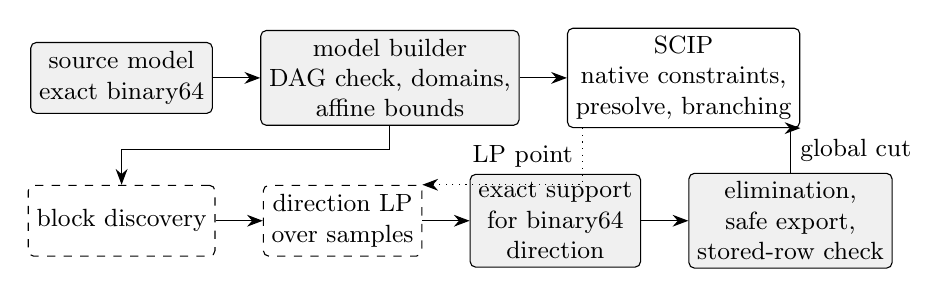
\begin{tikzpicture}[
  node distance=4mm and 6mm,
  box/.style={draw,rounded corners=2pt,align=center,font=\small,inner sep=3pt,minimum height=9mm},
  trusted/.style={box,fill=gray!12},
  num/.style={box,dashed},
  >={Stealth[length=2mm]}]
\node[trusted] (src) {source model\\exact binary64};
\node[trusted,right=of src] (bld) {model builder\\DAG check, domains,\\affine bounds};
\node[box,right=of bld] (scip) {SCIP\\native constraints,\\presolve, branching};
\node[num,below=9mm of src] (disc) {block discovery};
\node[num,right=of disc] (lp) {direction LP\\over samples};
\node[trusted,right=of lp] (sup) {exact support\\for binary64\\direction};
\node[trusted,right=of sup] (elim) {elimination,\\safe export,\\stored-row check};
\draw[->] (src) -- (bld);
\draw[->] (bld) -- (scip);
\draw[->] (bld.south) -- ++(0,-3mm) -| (disc.north);
\draw[->] (disc) -- (lp);
\draw[->] (lp) -- (sup);
\draw[->] (sup) -- (elim);
\draw[->] (elim.north) |- node[pos=0.25,right,font=\small] {global cut} (scip.south east);
\draw[->,dotted] (scip.south west) ++(2mm,0) |- node[pos=0.25,left,font=\small] {LP point} (lp.north east);
\end{tikzpicture}
\caption{Data flow of the separator. Shaded steps are part of the
certificate and are repeated by replay; dashed steps only choose what to
certify and need not be correct. SCIP's own computations are outside the
certificate.}
\label{fig:pipeline}
\end{figure}


\subsection{A faithful model}\label{sec:faithful}

A cut certificate refers to the model that the solver solves. Two ordinary
steps of model loading, assembling expressions and simplifying them, can
change that model without notice. We guard against both in every mode,
including the native baseline, so that all modes solve the same model. A
third paragraph describes the bounds that certificates use.

\paragraph{Arithmetic.}
Every finite binary64 number in the source file is interpreted as its exact
rational value. Assembling a native expression can still change values: in
$(0.1x)^2$ the source coefficient is the exact square of the binary64 number
$0.1$, whereas a coefficient computed in floating point is that square
rounded again, and a constraint constructor may move a constant to the other
side with a rounded subtraction. After assembly, the builder reads back the
PySCIPOpt expression object that it passes to SCIP and compares its exact
value with the source expression by symbolic subtraction and expansion, with
no tolerance. If they differ, it rebuilds the expression as an explicit
expression graph with separate constant nodes and compares again; a remaining
difference rejects the model. Constants are kept inside the expression, so
the constructor cannot round them into the row sides, which are passed
unchanged. This is translation validation
\citep{PnueliSiegelSingerman1998,Necula2000} of the model import. It
addresses the observation of \citet[Section~20]{Neumaier2004} that modeling
systems introduce uncontrolled rounding, and the requirement of
\citet[Section~3.1]{SchichlNeumaier2005} that simplification of an expression
graph introduce no roundoff. Its boundary is the expression object;
PySCIPOpt's translation of it into SCIP's internal expression, and SCIP's
later simplification, presolve and floating-point LP, are outside it.

\paragraph{Domains.}
Simplification can silently enlarge a domain: $0\cdot\log x$, $x/x$,
$(\sqrt x)^2$ and $(\log x)^0$ are defined only for $x>0$, $x\ne0$, $x\ge0$
and $x>0$, respectively. The builder visits every node of the source
expression before simplification and proves each domain requirement from
bounds and from affine rows; for example, $x-y=1$ proves that $\log(x-y)$ is
defined, with no bounds on $x$ and $y$. Requirements that cannot be proved
are enforced by existential constraints in a new variable $u$:
\[
d\ne0\iff\exists u:\ du=1,\qquad d>0\iff\exists u\ge0:\ du=1,\qquad d\ge0\ \text{is imposed directly.}
\]
The first is the device of \citet{Rabinowitsch1930}. Over the reals these
constraints describe strict domains exactly, without a positive tolerance
such as the one used in common benchmark setups \citep{BestuzhevaEtAl2025};
SCIP then enforces them, like every constraint, with its feasibility
tolerance. A variable power $b(x)^{e(x)}$ is admitted as $\exp(e(x)\log b(x))$
only when $b(x)>0$ is proved \citep[compare][]{BelottiEtAl2009}; otherwise
the model is rejected, because imposing $b>0$ could remove points at which
the power is defined for other reasons.

\paragraph{Bounds.}
Support domains need finite bounds. Original affine rows imply bounds that
may be missing from the declared box: for a row $\sum_ia_ix_i\le b$ with
$a_j\ne0$, $a_jx_j\le b-\sum_{i\ne j}\min\{a_i\ell_i,a_iu_i\}$. Any finite
sequence of such steps, with integer rounding for integer variables, yields
bounds that hold at every feasible point. Each step is recorded with its
source row, and replay repeats the sequence. The bounds are used only as
premises of certificates; the model keeps its declared bounds.

\subsection{Blocks, directions and activation}\label{sec:blocks}

Discovery runs at the first separator call, so a model solved during presolve
pays nothing. A ranged row $\ell\le g(v)\le u$ has two \emph{sides},
$g(v)\le u$ and $-g(v)\le-\ell$. Discovery writes each finite side of each
original row, including the objective epigraph row, exactly as a nonlinear
remainder plus an affine part. A side is admissible if its remainder involves
one to four variables with finite proven bounds and is either univariate or a
polynomial of total degree at most eight. Blocks are the variable sets of
single sides and greedy unions of overlapping sides, with at most four
variables, six nonlinear sides and sixteen signed affine domain sides; at
most 32 blocks are kept, in a fixed order with the largest first. Unsupported
remainders are declined as a whole, and a remainder is never altered. Affine
rows that involve only block variables, together with the proven bounds,
form the support domain $D$. Polynomial remainders of degree three or more in
three or four variables are admitted by discovery but are not certified by
any kernel (Bernstein bounds need one or two variables and at most 1{,}024
tensor coefficients), so such blocks yield no cuts.

At an LP solution the separator first tries, for each block and each of its
source sides $j$, the direction $a=0$, $\lambda=e_j$. This bounds only the
side's nonlinear remainder; the side's affine terms in the block variables
enter the cut only through the elimination. The support of the whole side,
with $a$ equal to the side's coefficients of the block variables, can be much
stronger; a variant that tries it first (\emph{whole-row directions}) is
evaluated in Section~\ref{sec:mechanism}. The
separator then solves up to three LPs that separate the current point, after
coordinate scaling, from the convex hull of sampled graph points plus the
cone of the side coordinates; an LP direction is used only if its scaled
violation exceeds $10^{-5}$. Samples are grid points of the box (33 points in
one variable, $7\times7$ in two, $3^d$ in $d=3,4$), plus the exact vertices of
the domain polytope and their centroid when the enumeration budget allows.
The binary64 values of $a$ and $\lambda$ are then certified. Quadratic blocks
are certified with Theorem~\ref{thm:polytope} when the number of row subsets
is at most 2{,}000; for four variables this allows at most seven signed
affine sides, and with at most sixteen sides the budget is never exceeded in
dimension three or less. Otherwise only the star oracle of
Theorem~\ref{thm:star} can apply, because the Bernstein bound is limited to
two variables and the ball-arithmetic bound to one; if the block is not a
star, that direction yields no cut. When an exact support computation returns
a minimizer that the samples missed, the minimizer is added and the LP is
solved again.

Two modes add cuts. Mode \code{all} tries the admitted blocks in their fixed
order until a cap is reached. Mode \code{auto} admits only quadratic blocks
that contain a side not proved convex and that have either an affine domain
row that is not a bound or at least two distinct nonlinear rows; it requires
a larger violation and stops trying a block after two failed certifications.
Both modes cap the number of callbacks, cuts and support calls
(Appendix~\ref{app:software}) and give all separator work a cumulative
allowance of $\min\{1\,\mathrm s,\,0.05\,T\}$ for a total budget $T$, checked
between operations; a single symbolic operation can overrun it. A cut is
added only if its violation divided by $\max\{1,\norm{\hat c}_1\}$ exceeds
$10^{-5}$ in \code{all} and $5\cdot10^{-4}$ in \code{auto}. Mode
\code{baseline} uses the same model builder and adds nothing. Modes with raised
limits and the variant with whole-row directions are listed in
Table~\ref{tab:modes}; we call the default first directions
\emph{remainder directions}.

\section{Computational study}\label{sec:computations}

The experiments address four questions: whether the stored cuts are valid in
practice, and what certification prevents; whether the cuts change SCIP's
results on benchmark models, including models that SCIP finds hard; what the
separator does and what it costs; and how much of the root gap the cuts close
on instances with the structure of Section~\ref{sec:composition}, compared
with SCIP's own alternatives and with Gurobi. We report four campaigns. Each
was run with code, limits and protocol fixed before its first run; we call
these results \emph{prospective}, and we label analyses designed after
results were seen as \emph{post hoc}. Campaigns 1 and~2 used earlier
implementations and are summarized in Appendix~\ref{app:campaigns12}.
Campaign~3 tests the final implementation on MINLPLib models (Parts~A and~B)
and on a constructed family (Part~C). Campaign~4 was designed after campaign~3
to answer the questions that its results raised: it adds comparators, fresh
instances, larger models, a variant of the family in which the block minima
do not give the optimum, and an ablation of the certificate. Table~\ref{tab:overview} lists the parts.

\subsection{Setup}\label{sec:setup}

All runs use SCIP~10.0.2 through PySCIPOpt~6.2.1 and Python~3.13, with one
SCIP thread and one BLAS thread per process, on a Linux host (WSL2) with 18
cores and 36 hardware threads that was shared with unrelated jobs; the
one-minute load average was 14 to 21 during the timed runs of campaign~3 and
about 3 to 8 during campaign~4. At most six runs of a campaign were active at a
time; the modes of one instance run back to back in
rotated order, and we compare modes only within such paired runs. Timings are
therefore descriptive. Times are in-process wall times charged to the soft
budget (model build, discovery, separation and solve), excluding interpreter
start-up and the primal check; \emph{SCIP time excluding the callback} is
SCIP's solving time minus the time spent in the separator callback. Gurobi
13.0.3 \citep{Gurobi13} solves the same model with one thread, its nonconvex
mode (\code{NonConvex=2}) and the same gap limit. Models
come from MINLPLib \citep{BussieckDrudMeeraus2003,Vigerske2026MINLPLib} in
OSiL format (Appendix~\ref{app:instances}), stratified by the library's
metadata into convex models, nonconvex models without integer variables, and
nonconvex models with integer variables.

A model counts as \emph{solved} if SCIP (or Gurobi) reports optimality or the
relative gap limit $10^{-4}$, and the returned incumbent passes an independent
check of all original rows, bounds, domains, integrality restrictions and the
objective at a scaled tolerance of $10^{-5}$; the checker evaluates the source
expressions without the model builder. Times are compared by shifted geometric
means (shift 1\,s) and by the median of per-run ratios, over runs solved in
every compared mode. Dual bounds $a$ and $b$ are compared with the tolerance
$10^{-4}\max\{1,\abs a,\abs b\}$, the gap limit. The \emph{root gap closed} by a
mode is $(z_{\text{mode}}-z_{\text{base}})/(z^\ast-z_{\text{base}})$ for
minimization, where $z$ denotes root dual bounds and $z^\ast$ the optimal or
best known value; for a run that ends at the root without reporting a root
bound, because the root node was pruned, $z$ is its final dual bound. Every recorded cut is replayed in a fresh process
(Section~\ref{sec:replay}). A run whose worker failed has no complete cut log;
its cut count is reported as unknown, not as zero.

\begin{table}[t]
\centering\footnotesize
\caption{Parts of campaigns 3 and 4. Full runs have a budget of 300\,s; root
runs have a node limit of one. All parts except 3D are prospective. Modes
are defined in Appendix~\ref{app:software} (Table~\ref{tab:modes}); ``extra''
is SCIP with its disabled nonconvex separators switched on.}\label{tab:overview}
\begin{tabular}{@{}l>{\raggedright\arraybackslash}p{0.33\textwidth}>{\raggedright\arraybackslash}p{0.43\textwidth}l@{}}
\toprule
Part & Instances & Modes & Runs\\
\midrule
3A & 30 MINLPLib models of campaign 2, seeds 0--2 & baseline, all, auto; root runs also all-diag & full, root\\
3B & 30 structure-selected models, seeds 0--1 & baseline, all, auto; root runs also all-diag & full, root\\
3C & 20 path-family instances & baseline, all-diag-mech & full, root\\
3D & as 3A--3C (post hoc) & whole-row variant & as 3A--3C\\
\midrule
4C2 & the 20 instances of 3C & checkvarlocks off, extra, frozen-wide, Gurobi & full, root\\
4C3 & 20 fresh path-family instances & baseline, all-diag-mech, rowdir-wide, extra, Gurobi & full, root\\
4C4 & the instances of 4C3 with a binding row & baseline, frozen-wide, rowdir-wide, extra, Gurobi & full, root\\
4B2 & the 30 models of 3B & no aggregation: baseline, all, all-diag, all-diag-rowdir; extra & root\\
4D & 20 larger models that SCIP finds hard & baseline, all, auto, extra; root runs also all-diag, all-diag-rowdir & full, root\\
4U & recorded cuts of campaigns 3 and 4 & uncertified constants & offline\\
4S & random stars with $10$ to $10^4$ leaves & two star algorithms & offline\\
\bottomrule
\end{tabular}
\end{table}

\subsection{Validity, and what certification prevents}\label{sec:validity}

Every recorded cut of campaigns 3 and~4 passed replay: 7{,}498 cuts in the
prospective parts of campaign~3, 30{,}998 in the post hoc diagnostic and
104{,}771 in campaign~4, 143{,}267 in total. In every part and cut mode, each of
the fourteen corrupted records of Section~\ref{sec:replay} was rejected. Every
incumbent returned in campaigns 3 and~4 passed the original-model check, with
one exception in a run without certified cuts: in a Part~D root run of SCIP
with its disabled separators switched on, the incumbent satisfied all
constraints, but SCIP's reported objective value differed by 34\% from the value
recomputed on the source model.

Two observations show that the checks are not idle. First, the stored-row
check (C4) rejected certified, violated rows in every part, because presolve
had aggregated or fixed a block variable or because SCIP had dropped or
rounded a coefficient (Section~\ref{sec:funnel}). Second, binary64 rounding
changed at least one coefficient in 13.5\% of the exported rows on the MINLPLib
models and in 92.5\% on the path family; the bound correction of
Proposition~\ref{prop:export} was at most $8.5\cdot10^{-16}$ in absolute value
and never destroyed a violation.

\begin{table}[t]
\centering\footnotesize
\caption{What an uncertified constant would have done. For the recorded
binary64 direction of each cut with an exact certificate, U1 is the minimum
over the separator's sample set and U2 the better of U1 and SLSQP local
minimizations. ``Wrong'' counts constants that exceed the exact support value
by more than $10^{-6}\max\{1,\abs{\text{value}}\}$; ``removes'' counts the
resulting rows that cut off an incumbent of the same model that passed the
original-model check; ``optimum'' counts rows that cut off the known optimal
solution. Path family: a random sample of 1{,}000 of the 138{,}000 recorded
cuts.}\label{tab:ablation}
\begin{tabular}{@{}llrrr@{}}
\toprule
Cuts & Constant & Wrong (models) & Removes (models) & Optimum\\
\midrule
MINLPLib, 5{,}116 cuts, 47 models & U1 & 1{,}969 (12) & 405 (7) & ---\\
 & U2 & 230 (4) & 132 (2) & ---\\
\midrule
Path family, 1{,}000 cuts, 60 instances & U1 & 976 (60) & 506 (58) & 404\\
 & U2 & 73 (37) & 27 (19) & 13\\
\bottomrule
\end{tabular}
\end{table}

To measure what the certificate itself buys, we recomputed, for the recorded
binary64 direction of each cut, the constant that an uncertified pipeline
would use instead of the certified support value (protocol Part~U): (U1) the
minimum over the separator's own sample set, which is what the direction LP
sees, and (U2) the better of U1 and local minimizations by SLSQP from the
three best samples, on the block box and the affine domain rows. Up to
binary64 rounding, both are upper bounds on the true support value.
Table~\ref{tab:ablation} compares them with the certified values. On the
MINLPLib models the sample minimum was wrong for 38\% of the cuts, and 405 of
the resulting rows would have cut off a feasible point that SCIP had returned
for the same model. Local minimization removed most of these errors but not
all. On \code{nvs02}, SLSQP stopped at its starting point after one iteration,
because the directional derivative along its first step was below its default
tolerance; on \code{kall\_ellipsoids\_tc02b} it started at stationary points
that are not local minima. On the path family, where the blocks are nonconvex
by construction, the sample minimum was wrong for almost every cut, 40\% of the
uncertified rows would have cut off the known optimal solution, and local
minimization still left rows that did so, because SLSQP converged to
non-global local minima. Every wrong constant is refuted by an explicit point:
the certified minimizer is exactly feasible and attains a smaller value. The
counts change little if the removal tolerance is raised tenfold. The certified
rows themselves were violated at recorded incumbents only within the
feasibility tolerance of these incumbents: for example, incumbents of
\code{st\_e22} with objective value $-85.0000017$, which satisfy the constraints
only up to a scaled violation of $10^{-8}$, violate the certified objective
bound $t\ge-85$, the true optimum, by $1.7\cdot10^{-6}$.

\subsection{MINLPLib models}\label{sec:minlplib}

Part~A repeats the 30 models of campaign~2 (ten per stratum, selected by a
hash ordering from 422 eligible models with at most 120 variables) with a
300-second budget, seeds 0, 1 and~2, and root runs. Part~B uses a sample
selected by structure: from the 392 eligible models not used in campaign~2,
the 111 on which discovery finds a block that the \code{auto} rule admits,
ranked by a hash, of which we take the first 30, with seeds 0 and~1. The root
runs of both parts include mode \code{all-diag}, whose raised limits test
whether the frozen limits, rather than the cuts, bound their effect. SCIP
solves most of these models in about a second, so they can show validity and
cost but hardly a benefit. Part~D, in campaign~4, addresses this: its pool
consists of the 322 MINLPLib models with more than 120 and at most 1{,}000
variables that are not convex by the library's metadata, contain a quadratic
or polynomial function and were not used before; 85 of them have a block that
\code{auto} admits, 58 of these are not solved by SCIP within 60 seconds, and
Part~D takes the first 20 of those in a fixed hash order
(Appendix~\ref{app:instances}). Table~\ref{tab:minlplib} summarizes the full
runs; Tables~\ref{tab:partA}, \ref{tab:partB} and~\ref{tab:partD} in
Appendix~\ref{app:instances} give the results per model.

\begin{table}[t]
\centering\footnotesize
\caption{Full runs on MINLPLib models (300\,s). Times are shifted geometric
means (shift 1\,s) over the runs solved by every mode of the part; ``SCIP
excl.'' is SCIP's solving time minus the separator callback; ``ratio'' is the
median per-run ratio of the total time to the baseline. ``Bounds'' counts
final dual bounds better/worse than the baseline at relative tolerance
$10^{-4}$ over all paired runs. In Part~D only two models were solved, and
times are not comparable.}\label{tab:minlplib}
\begin{tabular}{@{}llrrrrrr@{}}
\toprule
Part & Mode & Solved & Cuts (runs) & Time (s) & SCIP excl.\ (s) & Ratio & Bounds\\
\midrule
A (30 models, 3 seeds) & baseline & 80/90 & --- & 1.05 & 0.99 & --- & ---\\
  & \code{all}  & 80/90 & 151 (33) & 1.27 & 0.99 & 1.34 & 2/4\\
  & \code{auto} & 80/90 & 37 (15)  & 1.21 & 0.99 & 1.29 & 3/3\\
\midrule
B (30 models, 2 seeds) & baseline & 52/60 & --- & 1.33 & 1.27 & --- & ---\\
  & \code{all}  & 52/60 & 179 (40) & 1.87 & 1.25 & 2.66 & 2/0\\
  & \code{auto} & 52/60 & 145 (38) & 1.82 & 1.23 & 2.55 & 2/0\\
\midrule
D (20 models, 1 seed) & baseline & 2/20 & --- & & & & ---\\
  & \code{all}  & 2/20 & 14 (2) & & & & 5/1\\
  & \code{auto} & 2/20 & 14 (2) & & & & 4/0\\
  & \code{baseline-extra} & 1/20 & --- & & & & 7/7\\
\bottomrule
\end{tabular}
\end{table}

\paragraph{Parts A and B.} In every part and seed, all modes solved the same
models. In Part~A, cuts were added on 11 of the 30 models in mode \code{all}
and on 5 in mode \code{auto}. The final dual bounds of the 90 paired runs were
better in 2 and worse in 4 for \code{all}, and better in 3 and worse in 3 for
\code{auto}; between seeds, the baseline itself differed in 3 of 30
comparisons, so these differences are within run-to-run variation. In
Part~B, cuts were added on 20 of the 30 models; the final bounds were better
in 2 of 60 comparisons in each cut mode, both on \code{kall\_circles\_c8a} at
the time limit, and never worse. At the root the cuts had a visible effect on
four models of Part~B and none of Part~A. They closed the root gap of
\code{pooling\_bental4tp} in every cut mode and that of
\code{pooling\_bental4pq} in modes \code{auto} and \code{all-diag}, which were
then solved at the root, and they improved the root bounds of \code{ex3\_1\_4}
(from $-6$ to $-5.79$, and to $-5.69$ with raised limits; the optimum is $-4$)
and of \code{pointpack04}. In two root runs, \code{auto} ended with a worse root
bound, on \code{pointpack04} and on \code{pooling\_haverly2pq}, where the bound
fell from $-617.7$ to $-857.1$ (the optimum is $-600$). Valid cuts cannot
weaken an LP relaxation, but they change SCIP's later separation and cut
selection, and the bound at the end of the root node need not improve.
Raising the limits at the root (\code{all-diag}) added more cuts, 403 in
Part~A and 358 in Part~B, but improved the root bound beyond the tolerance on
only one more model in each part (\code{cvxnonsep\_psig20r} and
\code{pooling\_bental4pq}). None of these effects changed a full solve. The cut
modes were 15--20\% slower than the baseline in shifted geometric mean on
Part~A and 37--41\% on Part~B, and slower per run by median factors of 1.3 and
2.5--2.7. SCIP's own solving time, without the separator callback, was
unchanged (Table~\ref{tab:minlplib}), and the node counts summed over the
commonly solved runs differed by less than 3\%. The cuts are therefore neutral
for SCIP on these models, and the slowdown is the cost of the separator
(Section~\ref{sec:funnel}).

\paragraph{Presolve and the stored-row check (Part B2).} In campaign~3 the
stored-row check discarded 20\% (\code{all}) and 36\% (\code{all-diag}) of the
certified and violated rows of the Part~B root runs. Reruns that recorded the
cause showed that presolve had aggregated or fixed a block variable in 74--85\%
of these cases, so that SCIP stored the cut in other columns. Part~B2 repeats
the root runs with SCIP's aggregation and multi-aggregation disabled in every
mode. The rejected share fell to 5\% and 9.5\%; the remaining rejections come
from variables that presolve fixed and from SCIP's own coefficient handling
(integer snapping and coefficients below $10^{-9}$ dropped). Against SCIP with
the same presolve setting, mode \code{all} improved the root bound on 3 models
and worsened it on none, and \code{all-diag} improved it on 6 models
(including \code{pooling\_bental4tp}, \code{pooling\_bental4pq},
\code{ex3\_1\_4}, \code{sep1} and \code{pointpack04}) and worsened it on one
(\code{pooling\_haverly1tp}). Disabling aggregation, however, weakened SCIP's
own root bound on 6 of the 30 models, so the setting is not a free remedy. On
\code{kall\_circlespolygons\_c1p12}, where 127 of 152 violated rows had been
rejected before, 104 cuts now reached the LP, and the root bound stayed at $0$
against an optimum of $0.34$. Trying the support of each whole row first
(\code{all-diag-rowdir}) gave the same cuts and bounds on every model.

\paragraph{SCIP's disabled separators.} With its disabled-by-default nonconvex
separators switched on at the root (\code{baseline-extra}), SCIP improved the
root bound on 12 of the 30 Part~B models and worsened it on one
(\code{sep1}). It closed the root gap completely on five pooling and small
nonconvex models and by more than 95\% on two more, and these seven include
the four models on which the certified cuts had an effect; it solved 13 models
at the root against 8. Intersection cuts and interminor cuts were productive
on 26 and 21 models, edge-concave cuts on none. On these models, SCIP's own
alternatives are clearly stronger than the certified cuts.

\paragraph{Larger models (Part D).} In mode \code{all} the separator stopped
during block discovery on 12 of the 20 models, exactly those on which
discovery had taken more than the one-second allowance in the scan (1.0 to
7.7\,s). On six of the other eight it completed discovery and added no cut:
every certified support either fell below the violation threshold or, on three
models, was rejected by the stored-row check because presolve had fixed or
aggregated a block variable (11 of the 25 violated rows). With raised limits
at the root (\code{all-diag}), the separator added 891 cuts on 13 models and
improved the root bound on one model (\code{multiplants\_mtg1c}, closing 4\%
of its root gap), while the root bound was worse on five, by at most 3\% of the
gap; the variant with whole-row directions behaved the same. In the full runs
the cut modes solved the same two models as the baseline. All final-bound
differences in Table~\ref{tab:minlplib} occurred on models that received no
cut, so they reflect the changed timing of a time-limited run, not the cuts.
SCIP's disabled separators improved the root bound on 8 of the 20 models,
worsened it on 3, and in full runs lost one of the two solved models. On
models of this size the frozen separator rarely gets past discovery, and
where it does its cuts are not stronger than SCIP's relaxation.

\subsection{What the separator does and what it costs}\label{sec:funnel}

Table~\ref{tab:funnel} follows the certified rows from the support calls to
the cuts that reach SCIP. Three observations explain most of the results of
Section~\ref{sec:minlplib}.

\begin{table}[t]
\centering\footnotesize\setlength{\tabcolsep}{3.5pt}
\caption{Separator funnel, summed over the runs of a part and mode: support
calls, failed certifications, certified rows below the violation threshold,
rows rejected by the stored-row check, and cuts added; then the separator
callback time and its main parts. No row was ever discarded by safe rounding.
In the path family the separator runs only at the root, so full and root runs
have the same funnel; the times shown are those of the root runs. The three timed parts
do not add up to the total, which also contains untimed work.}\label{tab:funnel}
\begin{tabular}{@{}llrrrrrrrrr@{}}
\toprule
& & Support & Failed & Below & Stored-row & Cuts & \multicolumn{4}{c}{Callback time (s)}\\
\cmidrule(l){8-11}
Part & Mode & calls & cert. & thresh. & rejected & added & total & discovery & LPs & certif.\\
\midrule
3A full & \code{all} & 684 & 57 & 461 & 15 & 151 & 19.1 & 6.3 & 2.5 & 8.6\\
3B full & \code{all} & 884 & 14 & 646 & 45 & 179 & 32.9 & 4.4 & 3.9 & 23.0\\
3B root & \code{all-diag} & 1{,}618 & 19 & 1{,}039 & 202 & 358 & 45.1 & 2.3 & 9.6 & 30.4\\
4B2 root & \code{all-diag}, no aggr. & 1{,}572 & 17 & 1{,}058 & 47 & 450 & 38.6 & 2.1 & 8.6 & 25.7\\
4D root & \code{all} & 176 & 2 & 149 & 11 & 14 & 18.4 & 15.7 & 0.4 & 1.8\\
4D root & \code{all-diag} & 6{,}352 & 313 & 5{,}042 & 106 & 891 & 188.4 & 53.6 & 22.8 & 69.8\\
\midrule
3C & remainder, mech.\ limits & 3{,}462 & 0 & 391 & 71 & 3{,}000 & 73.6 & 10.6 & 9.6 & 32.0\\
4C2 & remainder, wide limits & 13{,}502 & 0 & 1{,}189 & 313 & 12{,}000 & 240.4 & 10.3 & 31.1 & 121.3\\
4C3 & whole row, wide limits & 15{,}534 & 0 & 3{,}181 & 353 & 12{,}000 & 269.2 & 10.3 & 32.6 & 140.1\\
4C4 & remainder, wide limits & 14{,}186 & 0 & 1{,}939 & 247 & 12{,}000 & 261.9 & 10.2 & 36.5 & 129.6\\
4C4 & whole row, wide limits & 15{,}204 & 0 & 2{,}989 & 215 & 12{,}000 & 274.8 & 10.7 & 36.6 & 137.7\\
\bottomrule
\end{tabular}
\end{table}

First, most certified supports are not violated at the LP point: on the
MINLPLib models, 65 to 86\% of the certified rows fell below the violation
threshold, because SCIP's relaxation already implied them up to the
threshold. Certification failed in few support calls. In the campaign-3 reruns
that recorded the outcome, every failure was \emph{incomplete} (a Bernstein
or ball-arithmetic bound reached its depth budget, or did not certify the
required value) or \emph{unsupported} (a quadratic block whose number of row
subsets exceeded the enumeration budget and which the fallback bounds do not
cover); none was an empty domain. In Part~D, 307 of the 313 failures came
from one model.

Second, the stored-row check lost a substantial share of the violated rows
on MINLPLib models, mainly to presolve aggregation (Section~\ref{sec:minlplib}),
and a small share on the path family, where SCIP dropped coefficients below
its epsilon of $10^{-9}$ in 2 to 3\% of the violated rows. Each such loss would be a
silent change of a certified row if the check were absent. A separator that
works in the presolved space, or that declares its variables
non-aggregatable before presolve, avoids most of the presolve losses; we did
the latter only as an experiment (Part~B2), because it changes SCIP's own
relaxation.

Third, on the MINLPLib models the whole slowdown is the separator's own time.
SCIP's solving time without the callback was unchanged in every part: its
shifted geometric mean differed from the baseline's by at most 4\% in
Parts~A and~B, and the median per-run ratio was between 0.96 and 1.01 in
Parts~B2 and~D. The callback cost about half a second per run in Part~B, more than SCIP's whole
solving time on most of these models (median 0.16\,s). In campaign~3, exact
certification took 70\% of the callback time on Part~B, the direction LPs and
discovery the rest; on the larger models of Part~D, discovery took 85\% of the
callback time in mode \code{all}. All of this is Python code; a compiled
implementation would remove most of it, but on these models it would at best
break even, because the cuts did not reduce SCIP's work. On the path family,
in contrast, the cuts reduced SCIP's own time sharply
(Section~\ref{sec:mechanism}), and the callback was the dominant remaining cost.

\subsection{A family with the path structure}\label{sec:mechanism}

The benchmark models do not tell whether the cuts can supply strength that
SCIP lacks where the theory predicts a gap. We therefore built a family with
the structure of Section~\ref{sec:interleave}. An instance with $n$ copies has
variables $x_i,y_i,z_i\in[0,1]$ and $t_i$, the rows
$\Phi^{(i)}(x_i,y_i,z_i)-t_i\le0$, where $\Phi^{(i)}$ is the
function~\eqref{eq:family} with $\omega_A=\omega_C=1$, one coupling row
$\sum_iy_i\le0.8n$, and the objective $\min\sum_it_i$. For each copy, four
distinct values are drawn from $\{k/64:k=0,\dots,48\}$ and split into two
interleaving two-point sets $A_i$ and $C_i$ with random orientation. All
coefficients are dyadic and exactly representable. Every optimal $y_i$ is a
midpoint of two values of at most $3/4$, so the coupling row does not bind, and
by Theorem~\ref{thm:interleave} the optimum is $\sum_i\delta_i^2/2$. Glued exact
pair hulls give the bound $0$ for every copy, so the part of the gap that only
the joint block closes is the whole optimum. Campaign~3 used five instances for
each $n\in\{10,20,40,80\}$ (seeds 0--4); campaign~4 adds five fresh instances
per $n$ (seeds 5--9), which no earlier run had used. The randomized family was
adopted after a pilot with native SCIP alone had shown that the deterministic
family, with every copy equal to the example of
Proposition~\ref{prop:path-gap}, is easy for SCIP: it solved $160$ copies in
19\,s.

Because the objective is a sum of block functions and the coupling row does not
bind, the $n$ cuts $t_i\ge\min\Phi^{(i)}$, which are the exact supports of the
blocks in the directions of their own rows, make the root bound equal to the
optimum. This is the most favorable case for block cuts. Part~C4 removes it: it
replaces the coupling row of each fresh instance by $\sum_iy_i\le c$, where $c$
is half the sum of the smallest unconstrained minimizers $y_i^\ast$, rounded down
to a multiple of $1/64$. The row then binds, the block minima no longer give the
optimum, and the cuts must be found in other directions. For C4 we know two
reference values exactly: the optimum, from a convex mixed-integer quadratic
reformulation solved by Gurobi and certified by an exact branch and bound; and
the best root bound that cuts on the blocks $(x_i,y_i,z_i)$ can give, which by
Theorem~\ref{thm:closure} and Corollary~\ref{cor:one-row} is
$\min\{\sum_i\operatorname{vex}\varphi_i(y_i):\sum_iy_i\le c,\ 0\le y\le1\}$
with $\varphi_i(y)=\dist(y,A_i)^2+\dist(y,C_i)^2$, computed with the exact convex
envelopes of the piecewise quadratic functions $\varphi_i$.
Table~\ref{tab:mechanism} summarizes the results; Tables~\ref{tab:path-detail}
and~\ref{tab:path-fresh} in Appendix~\ref{app:instances} give them per
instance.

\begin{table}[t]
\centering\footnotesize
\caption{The path family: median fraction of SCIP's default root gap closed,
$(z_{\text{mode}}-z_{\text{base}})/(z^\ast-z_{\text{base}})$, for each $n$ (five
instances each), and instances solved within 300\,s (of 20). ``Remainder'' and
``whole row'' are the first directions of the separator
(Section~\ref{sec:blocks}); ``mech.'' and ``wide'' are the limits of
Table~\ref{tab:modes}. The row ``glued pair hulls'' is the analytic bound~0 of
Theorem~\ref{thm:interleave}, which no run computes.}\label{tab:mechanism}
\begin{tabular}{@{}llrrrrr@{}}
\toprule
& & \multicolumn{4}{c}{Root gap closed (median)} & \\
\cmidrule(lr){3-6}
Instances & Mode & $n=10$ & $n=20$ & $n=40$ & $n=80$ & Solved\\
\midrule
seeds 0--4 & SCIP default & --- & --- & --- & --- & 9\\
 & SCIP, \code{checkvarlocks} off & 0.95 & 0.89 & 0.93 & 0.91 & 10\\
 & SCIP, disabled separators on & 0.64 & 0.58 & 0.66 & 0.59 & 10\\
 & Gurobi & & & & & 7\\
 & glued pair hulls & 0.95 & 0.89 & 0.94 & 0.92 & \\
 & remainder, mech.\ (campaign 3) & 0.35 & 0.25 & 0.19 & 0.22 & 9\\
 & remainder, wide & 0.86 & 0.87 & 0.89 & 0.90 & 13\\
 & whole row, mech.\ (post hoc) & 0.44 & 0.44 & 0.43 & 0.46 & 10\\
 & whole row, wide (post hoc) & 1.00 & 1.00 & 1.00 & 1.00 & 20\\
\midrule
seeds 5--9 & SCIP default & --- & --- & --- & --- & 9\\
 & SCIP, disabled separators on & 0.57 & 0.64 & 0.61 & 0.66 & 9\\
 & Gurobi & & & & & 5\\
 & glued pair hulls & 0.93 & 0.92 & 0.93 & 0.92 & \\
 & remainder, mech. & 0.32 & 0.31 & 0.24 & 0.21 & 10\\
 & whole row, wide & 1.00 & 1.00 & 1.00 & 1.00 & 20\\
\midrule
binding row & SCIP default & --- & --- & --- & --- & 10\\
(seeds 5--9) & SCIP, disabled separators on & 0.29 & 0.60 & 0.68 & 0.65 & 13\\
 & Gurobi & & & & & 6\\
 & remainder, wide & 0.98 & 0.96 & 0.95 & 0.93 & 20\\
 & whole row, wide & 0.997 & 0.99 & 0.98 & 0.98 & 20\\
\bottomrule
\end{tabular}
\end{table}

\paragraph{SCIP's root bound and the pair-hull level.} SCIP's default root
bound is weak: on the instances of campaign~3 it lies between $-0.035$ and
$-0.013$ per copy, while each copy contributes at least $1/8192$ to the optimum. The
cause is a presolve step: $\Phi^{(i)}$ is concave in $x_i$ and in $z_i$, so
SCIP's implicit-discreteness detection \citep[Section~4.2.7]{SCIP8report} makes
these variables binary, and SCIP then closes the gap by branching. With this
step disabled (\code{constraints/nonlinear/checkvarlocks = d}), SCIP's root bound
rises to just below~0, the bound of glued exact pair hulls, on every instance
of campaign~3 (Table~\ref{tab:mechanism}); SCIP's semidefinite minor cuts were
productive in all of these runs and in none of the default runs of campaign~4. Native SCIP thus reaches the
pair-hull level when presolve does not interfere, and no SCIP setting closed
any part of the gap between this level and the optimum, which is the gap that
Section~\ref{sec:composition} attributes to joint blocks. SCIP's disabled
separators, of which only the intersection cuts were productive, closed about
60\% of the default root gap. Gurobi~13 solved the instances with $n=10$ and
two with $n=20$; on $n=40$ and $n=80$ its gap after 300\,s was 53 to 121\%.

\paragraph{The prospective separator and the attribution.} The separator of
campaign~3 improved the root bound on all 20 instances but closed only a median
of 19--35\% of the root gap, less than the pair-hull level, and it solved the
same 9 instances as SCIP; on these, it reduced the number of nodes and the
shifted geometric mean time from 10.3\,s to 6.7\,s. After seeing these results
we found two causes. The first directions of the separator bound only the
nonlinear remainder of a row (Section~\ref{sec:blocks}), whereas the exact
support of the whole row is the block minimum, and the $n$ cuts
$t_i\ge\min\Phi^{(i)}$ give the optimum. In addition, the first blocks of a
callback take up to four cuts each, so with $n$ cuts per callback the later
blocks receive none. A post hoc diagnostic, designed after these results and
reported separately, tried the whole-row direction first, with the same limits
and with four times as many cuts per callback and in total and twice as many
support calls. Before it, we had
checked the wide limits by hand on two of the 20 instances. The whole-row
direction alone raised the median closure to 43--46\% and solved one more
instance; together with the wide
limits it closed the root gap on all 20 instances, and all 20 were solved, 12
of them at the root node. Campaign~4 added the missing cell of this $2\times2$
design prospectively: with the remainder directions and the wide limits, the
separator closed 86--90\% of the gap, close to the pair-hull level and above
it on 7 of the 20 instances, and solved 13. The campaign-4 runs had a less loaded
host than those of campaign~3, but this does not explain the difference: every
run of the four cells stopped at its cut cap, so the root bounds do not depend
on time, and the four additional instances were solved in 9 to 168\,s. The
limits therefore account for most of the closure, and the whole-row
directions for the part beyond the pair-hull level.

\paragraph{Prospective test on fresh instances.} On the 20 instances with
seeds 5--9, the whole-row variant with wide limits, fixed before these
instances were generated, closed the root gap on every instance: its root
bound was within $2\cdot10^{-7}$ of the optimum. It solved all 20 in 3 to 33\,s,
with a median of one node and at most 38, against 9 for SCIP, 9
for SCIP with its disabled separators, 10 for the separator with remainder directions and mechanism limits, and 5 for
Gurobi. On the nine instances that SCIP solved, the total time was comparable
(median ratio 0.86), while SCIP's own time fell to a median of 4\% of its time
in the baseline; over all 20 runs, 96\% of the time was spent in the Python
separator. The separator with remainder directions and mechanism limits
closed 21--32\% of the root gap, as in campaign~3.

\paragraph{A binding coupling row (Part C4).} When the coupling row binds,
the block minima no longer give the optimum, and the cuts must have the right
slopes in $y_i$. Both separator configurations with wide limits solved all 20
instances, in 3 to 134\,s, against 10 for SCIP, 13 for SCIP with its disabled
separators and 6 for Gurobi; only the cut modes solved any instance with
$n=80$. On the ten instances that SCIP solved, all with $n\le20$, the cut
modes were slower by median factors of 3.2 and 3.5, because of the
separator's time. At the root they closed a median of 95\% (remainder directions) and 99\%
(whole-row directions) of SCIP's root gap. Here the reference that matters is
the best root bound that cuts on the blocks can give, which equals the optimum
on 13 of the 20 instances and lies at most $6.5\cdot10^{-4}$ below it on the
others; no root run reached it, and the remaining distance grew with $n$, to
between 0.016 and 0.029 for $n=80$ with whole-row directions. Every cut-mode run
stopped at its cap of $16n$ cuts, so a larger cap would probably close more. The
cuts that did the work came from the LP direction search: 99.9\% (remainder directions) and
94\% (whole row) of the cuts were LP directions, and almost all of them have a
nonzero coefficient of $y_i$, mostly with the negative slope that the binding
row requires; the whole-row cuts alone give only $\sum_i\min\varphi_i$, which is
below SCIP's root bound on half of the instances. The direction search can
therefore find useful non-row directions, but on these instances it needed
about $16$ cuts per block to come close to the block closure, and none of the
cuts is an envelope cut in $(y_i,t_i)$ alone.

These families were constructed to have the structure of
Section~\ref{sec:composition}, and their objectives are sums of block
functions, which favors block cuts. They show that exact block support
supplies strength that neither SCIP, with or without its disabled separators,
nor Gurobi obtains at the root, that this strength reaches the solver only if
the direction search tries the right directions and enough of them, and that
on such instances it can turn time-outs into solves at or near the root. They
are not evidence about other models.

\subsection{The star oracle at scale}\label{sec:star-bench}

No block of Sections~\ref{sec:minlplib}--\ref{sec:mechanism} had more than
four variables, so the star algorithm of Theorem~\ref{thm:star} was not needed
there. Part~S measures it directly, without a solver, on random constrained
stars with $k\in\{10,100,1000,10000\}$ leaves (five instances each), $2k$
center--leaf rows, one to three rows in the center alone, and small rational
coefficients of both signs, so that convex, concave and affine leaves occur.
We compare an implementation of the sweep of the proof with the simpler star
oracle of our separator (Section~\ref{sec:star}). Where both ran ($k\le1000$),
the two minima were equal as rational numbers, and on all 20 instances the
sweep's minimizer was exactly feasible and attained the reported value. The
sweep took a median of 1.3\,ms, 12\,ms, 0.17\,s and 2.1\,s of CPU time for the
four values of $k$, close to linear growth, whereas the simpler oracle took
6\,ms, 0.43\,s and 29\,s for $k\le1000$, growing by a factor of about 70 per
tenfold increase in $k$; at $k=10^4$ it was not run, because its extrapolated
time exceeded ten minutes per instance. Its partitions had about twice as
many pieces as the sweep's (median 900 against 416 at $k=1000$). The minima
had numerators and denominators of at most 94 and 78 bits, with no steady
growth in $k$, in line with the size bounds of Appendix~\ref{app:star}.

\subsection{Summary and limitations}\label{sec:comp-summary}

Every one of the 143{,}267 recorded cuts passed replay against the source
model and the row stored by SCIP, whereas constants computed without a
certificate would have cut off feasible points on seven MINLPLib models and on
58 of the 60 sampled path-family instances, often the known optimal solution. On MINLPLib models the
cuts were neutral for SCIP: they never changed which models it solved in
campaigns 2 to~4, and they left SCIP's own solving time unchanged. The
Python separator's overhead made the runs slower, and SCIP's own
disabled-by-default separators improved the root bound more often than the
certified cuts did. On constructed families with the path structure, a
separator configuration fixed in advance closed all or nearly all of the root
gap and solved all instances, with a non-binding and with a binding coupling row, where SCIP,
SCIP with its disabled separators and Gurobi solved at most two thirds of them.
We therefore do not recommend enabling the separator by default; its value is
on models whose joint block structure SCIP's relaxation misses, and an
activation rule that recognizes such models is not available.

The study has limitations that the reader should weigh. The MINLPLib parts use
models with at most 1{,}000 variables and blocks with at most four variables;
larger blocks, where the star algorithm would matter, did not occur within the
frozen limits. The implementation is in Python, so the measured cost is an
upper bound on that of a compiled separator. The host was shared, with
different loads in campaigns 3 and~4, so we compare times only within paired
runs of one campaign, and time differences of a few percent are not
meaningful \citep{LodiTramontani2013}. Runs used one seed, except Parts~A and~B,
and one thread. Gurobi was run with one thread and default settings apart from
its nonconvex mode. The path families are constructed and favor block cuts; the
post hoc diagnostic of campaign~3 was designed after its results were seen, and
its finding was then tested prospectively on fresh instances.


\section{Discussion and conclusions}\label{sec:conclusions}

Two consequences of the theory matter for solver design. First,
certification does not constrain how directions are found: only the final
binary64 row, its bound over the whole block domain and the row that the
solver stores need to be checked, and all of this can be replayed. Second,
the advantage of joint quadratic blocks over their pairs is one of
representation. Pair hulls glued on finitely many moments of a shared
variable accept distributions that no joint distribution reproduces, and they
give the trivial bound zero exactly when the local zero sets alternate often
enough; dense moment relaxations with products that are absent from the model
close the same gaps, and support cuts obtain that strength in the model's own
coordinates. For stars, the most common merged blocks, the support problem
remains exactly solvable in nearly linear time when rows couple the center
with one leaf at a time.

The computations sharpen these conclusions. Certification is a real
safeguard, not a formality: constants taken from samples or from a local
solver were wrong for a large share of the cuts and would have cut off
feasible solutions, including known optima, while every certified cut
replayed. The stored-row check exposed an obstacle that the theory does not
see: presolve aggregates or fixes the variables to which a block refers, so a
separator stated in the original variables loses cuts unless it works in the
presolved space or prevents these reductions, and preventing them weakens
SCIP's own relaxation. On MINLPLib models the cuts were neutral for SCIP, and
SCIP's disabled-by-default separators were stronger, so the cost of the
separator was overhead. On the constructed families, where the theory predicts
a gap, the picture is the opposite. Native SCIP reached the level of glued pair
relaxations once one presolve step was disabled and went no further, and the
certified cuts closed the gap beyond that level and solved every instance. They
did so only with the exact support of each whole row as a first direction,
enough cuts per block, and, when a coupling row binds, a direction search that
finds sloped cuts.

Several questions remain open. Exact support for trees deeper than stars with
edge-local rows would extend the star algorithm to the structures of network
models; Remark~\ref{rem:trees} shows that the rational partition argument
does not extend directly. Proposition~\ref{prop:gain}(ii) reduces the gap of
the glued relaxation in any direction to a concave maximization over
re-splittings, but which directions to merge, and when merging pays off, is
not answered by it. A direction search with the guarantees of
Appendix~\ref{app:separation} and the speed of a solver callback is not
available; on the binding-coupling family the search needed about sixteen cuts
per block to approach the block closure. Finally, an activation rule that
predicts when joint cuts pay off would be needed before any default use; our
structural rule did not achieve this, and on our MINLPLib samples SCIP's own
relaxation already contained what the cuts could add.

\section*{Code and data availability}\label{sec:availability}
\addcontentsline{toc}{section}{Code and data availability}

The supplementary archive of this article contains the separator and the
model builder, the replay checker, the frozen code snapshots of every
campaign with their SHA-256 manifests, the protocols, the job lists and
instance selections, the run records and logs, the replay outputs, the
scripts that produce every table and number of Section~\ref{sec:computations}
from the records, and the verification scripts for the theorems and examples
(exact rational and symbolic checks). The experiments used SCIP~10.0.2
through PySCIPOpt~6.2.1, Python~3.13.11, SymPy~1.14.0, python-flint~0.9.0
(Arb), SciPy~1.18.1 (HiGHS for the direction LPs) and Gurobi~13.0.3, and a
local copy of MINLPLib \citep{BussieckDrudMeeraus2003,Vigerske2026MINLPLib}
whose files are archived with their hashes. Replay needs Python with SymPy,
python-flint and PySCIPOpt; it constructs, but does not solve, a SCIP model.


\bibliographystyle{plainnat}
\bibliography{references}

\appendix
\section{Exact quadratic support on polytopes}\label{app:polytope}

\subsection{Proof of Theorem~\ref{thm:polytope}}

Every candidate lies in $P$, so an empty $P$ has none. Assume $P\ne\emptyset$.
Among the global minimizers, which exist by compactness, choose $x^\ast$ such
that the face $G$ of $P$ with $x^\ast\in\relint G$ has the smallest dimension,
and let $V$ be the linear space parallel to $\aff G$. Because $x^\ast$
minimizes $q$ over $G$ and lies in its relative interior,
$v\T(Hx^\ast+c)=0$ and $v\T Hv\ge0$ for all $v\in V$.

Suppose $v\in V\setminus\{0\}$ satisfies $v\T Hv=0$. Then $q(x^\ast+tv)=q(x^\ast)$
for all $t$. The line $x^\ast+tv$ meets the bounded face $G$ in a segment that
contains $x^\ast$ in its relative interior, and an endpoint of the segment is
a global minimizer on a proper face of $G$, which contradicts the choice of
$x^\ast$. Hence $H$ is positive definite on $V$, or $V=\{0\}$.

Let $J$ be the set of rows active at $x^\ast$, so that
$\aff G=\{x:A_Jx=b_J\}$ and $V=\ker A_J$, and let $I\subseteq J$ index a basis
of the row space of $A_J$. Then $\abs I\le d$ and $\ker A_I=V$. Since
$Hx^\ast+c$ is orthogonal to $V$, it lies in the row space of $A_I$, so
$(x^\ast,\mu)$ solves~\eqref{eq:kkt-system} for some $\mu$. If $M_I(v,\nu)=0$,
then $A_Iv=0$, so $v\in V$, and $v\T Hv=-v\T A_I\T\nu=0$; hence $v=0$, and
$A_I\T\nu=0$ gives $\nu=0$ by independence. So $M_I$ is nonsingular, its unique
solution contains $x^\ast$, and $x^\ast$ is a candidate. All data are rational,
so the candidates and their values are rational. A set of dependent rows
never gives a nonsingular $M_I$, so enumerating independent sets suffices.
\qed

\subsection{Encoding lengths}

Multiply each row of $Ax\le b$ by the product of the denominators of its
entries, and multiply $q$ by the product $\sigma$ of the denominators of its
coefficients. Positive row scalings and $\sigma>0$ change neither $P$, nor the
nonsingularity of $M_I$, nor the $x$-part of its solution. Afterwards all row
entries are integers of absolute value at most $2^{\langle A\rangle}$ and all
entries of $\sigma H$ and $\sigma c$ are integers of absolute value at most
$2^{\langle q\rangle+1}$; write $\alpha=\langle A\rangle$ and
$\eta=\langle q\rangle+1$.

Let $\abs I=s\le d$ and $n=d+s$. Scale the last $s$ rows and the last $s$
columns of the integer matrix $[M_I\mid(-\sigma c,b_I)]$ by $2^{-\alpha}$. In
the scaled matrix, the first $d$ rows have entries of absolute value at most
$2^\eta$ and the others at most $1$. Hadamard's inequality applied to any
square submatrix of order at most $n$, and the undoing of the scaling, give
\[
\abs{\det N}\le n^{n/2}2^{d\eta+2s\alpha}\le B:=(2d)^d2^{d(\eta+2\alpha)}
\]
for every square submatrix $N$ of $[M_I\mid(-\sigma c,b_I)]$. By Cramer's rule a
candidate has coordinates $x_j=N_j/\Lambda$ with $\abs{N_j},\abs\Lambda\le B$.
Writing $\sigma q=\tilde c_0+\sum_j\tilde c_jx_j+\sum_{i\le j}\tilde Q_{ij}x_ix_j$
with integer coefficients bounded by $2^\eta$,
\[
\sigma q(x)=\frac{\Lambda^2\tilde c_0+\Lambda\sum_j\tilde c_jN_j+\sum_{i\le j}\tilde Q_{ij}N_iN_j}{\Lambda^2},
\]
a numerator with at most $(d+1)^2$ terms, each bounded by $2^\eta B^2$. So
$\min_Pq$ is a fraction whose numerator and denominator are bounded by
$(d+1)^22^{\eta}B^2$ and $2^{\eta}B^2$. Hence every candidate and the minimum
have bit length $O(d(\langle q\rangle+\langle A\rangle+\log d))$, for every $d$.

Bareiss's fraction-free elimination keeps every intermediate number equal to
a minor of the matrix above, and the products formed before each exact
division are bounded by $2B^2$. Feasibility tests and value comparisons are
integer comparisons of numbers bounded by $(d+1)2^\alpha B$ and
$(d+1)^22^\eta B^4$. The total work is $O(N(m,d)(d^3+md))$ arithmetic
operations on integers of bit length $O(d(\langle q\rangle+\langle A\rangle+\log d))$.
For fixed $d$, $N(m,d)\le(m+1)^d$, the number of arithmetic operations does
not depend on the sizes of the numbers, and the algorithm is strongly
polynomial.

\subsection{Proof of Proposition~\ref{prop:maxcut}}

For a graph $G=(V,E)$ let $q(x)=-\sum_{\{i,j\}\in E}(x_i+x_j-2x_ix_j)$. Since
$q$ is affine in each coordinate, moving coordinates one at a time to a
minimizing endpoint does not increase $q$, so some minimizer is binary. At a
binary point the summand of an edge equals one exactly when the edge crosses
the cut defined by $x$, so $\min q$ is minus the maximum cut size, and
unweighted MAX CUT is NP-hard \citep{Karp1972,GareyJohnsonStockmeyer1976}. The
coefficients are integers of absolute value at most $n$. For the second
statement, membership in coNP follows because a violating point can be taken
to be a candidate of Theorem~\ref{thm:polytope}, which has polynomial size.
For the hardness, $\min q$ is an integer for the quadratic $q$ of the
reduction, because $q$ has integer coefficients and a binary minimizer; hence
$\min q\le-W$ holds if and only if $q\ge-W+\tfrac12$ fails on $[0,1]^n$. \qed

\section{Sizes, a lower bound and a depth-two example for stars}\label{app:star}

For a rational $r=p/q$ in lowest terms let $\operatorname{ht}(r)=\log_2\max\{\abs p,q\}$.
Then $\operatorname{ht}(rs),\operatorname{ht}(r/s)\le\operatorname{ht}(r)+\operatorname{ht}(s)$
and $\operatorname{ht}(r_1+\dots+r_N)\le\log_2N+\sum_j\operatorname{ht}(r_j)$. Let
$\tau_i$ bound $\operatorname{ht}$ over the data of leaf $i$ (its coefficients,
bounds and rows), $\tau_0$ over the center data (its coefficients, bounds and
the rows in $y$ alone), and $\tau=\max_{0\le i\le k}\tau_i$.

\paragraph{Sizes.}
The coefficients of the affine functions defining $L_i$ and $U_i$ have
$\operatorname{ht}\le2\tau_i$, and $v_i$ has $\operatorname{ht}\le2\tau_i+1$. A
breakpoint is the intersection of two such functions or the zero of the affine
factor in~\eqref{eq:endpoint-factor}; in both cases $\operatorname{ht}\le12\tau+4$,
independently of $k$. The endpoints of $I$ are bounds of $y$, zeros of rows in
$y$ alone ($\operatorname{ht}\le2\tau_0$) or intersections of two lines of one
leaf, so they obey the same bound. On a piece, the contribution of leaf $i$ to
$V$ is a quadratic in $y$ whose coefficients have $\operatorname{ht}\le11\tau_i+7$,
so the coefficients of $V$, which are sums of $k+1$ such terms, have
$\operatorname{ht}\le C:=\log_2(k+1)+\tau_0+\sum_i(11\tau_i+7)$, which is linear in
the input length. Evaluating at a breakpoint, at an endpoint of $I$ or at a
stationary point $-c_1/(2c_2)$ gives a minimum with $\operatorname{ht}\le4C+36\tau+14$.
Because the sweep updates the coefficients exactly, every running sum equals
the coefficient of the current piece and obeys the same bound. The algorithm
is therefore strongly polynomial.

\paragraph{Lower bound.}
Ben-Or's theorem states that an algebraic computation tree deciding membership
in a set $W\subseteq\R^n$ with $N$ connected components has depth
$\Omega(\log N-n)$ \citep{BenOr1983}. For $r\ge1$ let
$W=\{z\in(0,2r)^r:\abs{z_i-z_j}\ge1\ \text{for}\ i\ne j\}$, which has one component
for each of the $r!$ orderings. For $z\in(0,2r)^r$ build a star with center
$y\in[0,2r]$ and, for each $j$, three leaves: $x\in[0,1]$ with objective
$(y-z_j+1)x$; $x\in[0,1]$ with objective $(z_j+1-y)x$; and $x\in[0,2r+1]$ with
the row $x\ge y-z_j$ and objective $2x$; add the center terms
$-ry+\sum_jz_j-r$. With $t=y-z_j$, the identity
$\min\{0,t+1\}+\min\{0,1-t\}+2\max\{0,t\}-t-1=-\max\{0,1-\abs t\}$ shows that
$V(y)=-\sum_j\max\{0,1-\abs{y-z_j}\}$, a sum of negative tents of width two. If
$z\in W$, at most two tents are positive at any $y$ and their sum is at most
one, so $\min V\ge-1$; if $\abs{z_i-z_j}<1$, then $V<-1$ at the midpoint of $z_i$
and $z_j$. The instance has $3r$ leaves and $r$ leaf rows and is computed from
$z$ with $O(r)$ operations, so deciding $\min V\ge-1$ needs depth
$\Omega(r\log r)$.

\paragraph{Depth two.}
For $f=(x_2-\tfrac18)x_1+x_2^2-x_2+x_2x_3+x_3^2-x_3$ on $[0,1]^3$, minimizing over
$x_1$ first gives $\min\{0,x_2-\tfrac18\}+x_2^2+(t-1)x_2$ with $t=x_3$. On
$[0,\tfrac18]$ its minimum is $-\tfrac18$ at $x_2=0$; on $[\tfrac18,1]$ it is
$-\tfrac14(1-t)^2$ at $x_2=(1-t)/2$ when $t\le\tfrac34$, and larger than $-\tfrac18$
otherwise. Hence the conditional value is $\min\{-\tfrac18,-\tfrac14(1-t)^2\}$,
whose two pieces meet at $t=1-\sqrt2/2$, a root of $2t^2-4t+1$. Adding $t^2-t$
and minimizing over $t\in[0,1]$ gives $\min f=-\tfrac38$ at $(1,0,\tfrac12)$.

\section{Proof details for Section~\ref{sec:composition}}\label{app:composition}

\subsection{Lower bounds for Theorem~\ref{thm:interleave}}\label{app:interleave}

Let $\nu_A$ and $\nu_C$ be probability measures on $[\ell,u]$ with equal moments
of orders one and two. For any polynomial $p$ of degree at most two,
$\int\dist(y,A)^2d\nu_A+\int\dist(y,C)^2d\nu_C$ equals
$\int(\dist(y,A)^2-p)\,d\nu_A+\int(\dist(y,C)^2+p)\,d\nu_C$, so it suffices to
find $p$ with $\dist(\cdot,A)^2-p\ge\kappa_A$ and $\dist(\cdot,C)^2+p\ge\kappa_C$ on
$\R$ and $\kappa_A+\kappa_C=\delta^2/2$. Because $\dist(y,S)^2=\min_{s\in S}(y-s)^2$,
each inequality can be checked one point $s$ at a time. We use
$\inf_y[\alpha(y-s)^2+\beta(y-t)^2]=\alpha\beta(s-t)^2/(\alpha+\beta)$ for
$\alpha+\beta>0$.

\emph{Separated sets.} By symmetry let $\max A<\min C$, put $a_0=\max A$,
$c_0=\min C$, $\delta=c_0-a_0$, $t_0=(a_0+c_0)/2$ and $p(y)=\delta(y-t_0)$. For
$s\in A$, $\inf_y[(y-s)^2-\delta(y-t_0)]=-\delta^2/4-\delta(s-t_0)\ge\delta^2/4$, and
for $t\in C$, $\inf_y[(y-t)^2+\delta(y-t_0)]=-\delta^2/4+\delta(t-t_0)\ge\delta^2/4$.

\emph{Nested sets.} By symmetry let $C$ lie strictly between the two points
$a_-<a_+$ of $A$. Put $t_0=(\min C+\max C)/2$, $h=(\max C-\min C)/2$ and
$\rho=\delta+h$; then $\abs{s-t_0}\ge\rho$ for $s\in A$ and $\abs{t-t_0}\le h$ for
$t\in C$. If $h>0$, let $\gamma=(\rho-h)/(\rho+h)\in(0,1)$ and
$p(y)=-\gamma(y-t_0)^2$. Then
$\inf_y[(y-s)^2+\gamma(y-t_0)^2]=\gamma(s-t_0)^2/(1+\gamma)\ge\gamma\rho^2/(1+\gamma)$ and
$\inf_y[(y-t)^2-\gamma(y-t_0)^2]=-\gamma(t-t_0)^2/(1-\gamma)\ge-\gamma h^2/(1-\gamma)$.
With $1+\gamma=2\rho/(\rho+h)$ and $1-\gamma=2h/(\rho+h)$ the two bounds add up to
$(\rho-h)^2/2=\delta^2/2$. If $h=0$, take $p(y)=-(y-t_0)^2$; then
$\dist(\cdot,C)^2+p\equiv0$ and $\dist(\cdot,A)^2-p\ge\delta^2/2$.

\subsection{A separating polynomial for Theorem~\ref{thm:alternation}}\label{app:alternation}

Let $A$ and $C$ be disjoint, nonempty and compact, let $T=A\cup C$, and define
the label $\epsilon(t)=+1$ for $t\in A$ and $\epsilon(t)=-1$ for $t\in C$. Let
$\varepsilon=\dist(A,C)>0$. Starting from $s_0=\min T$, let $s_{i+1}$ be the
smallest point of $T$ larger than $s_i$ with the opposite label, as long as
one exists. Such a point exceeds $s_i$ by at least $\varepsilon$, so the
process stops at some $s_r$, and every point of $T$ in $[s_i,s_{i+1})$ has the
label of $s_i$. Every alternating chain visits these runs in increasing
order, so $\operatorname{alt}(A,C)=r$. Let $e_i$ be the largest point of $T$
in $[s_{i-1},s_i)$ and choose $\rho_i\in(e_i,s_i)$. Then
$p(t)=\epsilon(s_0)\prod_{i=1}^r(\rho_i-t)$ has degree $r$, and a point of the
$i$-th run lies between $\rho_i$ and $\rho_{i+1}$, so $\operatorname{sign}p(t)=\epsilon(t)$:
$p>0$ on $A$ and $p<0$ on $C$. If $r\le\kappa$, then $\int p\,d\alpha=\int p\,d\gamma$
for any probability measures $\alpha$ on $A$ and $\gamma$ on $C$ with equal
moments up to order $\kappa$, which is impossible.

\subsection{Dense moment matrices for the path family}\label{app:sdp}

We use the notation of Theorem~\ref{thm:interleave}, assume that $A$ and $C$
interleave, and let $v\in R$ be a point with $\operatorname{lin}\Phi(v)=0$. Let
$M$ be the moment matrix of $(1,x,y,z)$ with the entries of $v$ and an
unspecified entry $p_{xz}$.

\emph{The dense moment matrix alone does not exclude $v$.} The specified
entries of $M$ form a chordal pattern whose two maximal blocks, the moment
matrices of $(1,x,y)$ and $(1,y,z)$, are positive semidefinite because the two
parts of $v$ are moment vectors. Hence $M$ has a positive semidefinite
completion \citep{GroneEtAl1984}, and $v$ together with this completion
satisfies the dense moment constraint and all RLT inequalities of the edges
and squares.

\emph{The McCormick inequalities of $xz$ alone do not exclude $v$.} They
require $\max\{0,m_x+m_z-1\}\le p_{xz}\le\min\{m_x,m_z\}$, an interval that is
nonempty for $m_x,m_z\in[0,1]$.

\emph{Together they exclude it.} Replacing $x$ by $1-x$ exchanges $a_1$ and $a_2$
and maps the four McCormick inequalities of $xz$ to each other, and similarly
for $z$, so we may assume $a_1<a_2$ and $c_1<c_2$. The $(x,y)$ part of $v$ is
the moment vector of a measure supported on the zero set of $\Phi_A$, which is
$\{(0,a_1),(1,a_2)\}$: at a point with $0<x<1$, concavity or affinity in $x$
gives $\Phi_A(x,y)\ge(1-x)(y-a_1)^2+x(y-a_2)^2>0$. Hence $x=\alpha+\beta y$ on this
support, with $\beta=1/(a_2-a_1)$ and $\alpha=-a_1\beta$, and the vector
$w=(\alpha,-1,\beta,0)$ satisfies $w\T Mw=0$. If $M\succeq0$, then $Mw=0$, and the
last row gives $p_{xz}=\alpha m_z+\beta p_{yz}$; so the completion is unique. In
the same way $z=(y-c_1)/(c_2-c_1)$ on the $(y,z)$ support, which gives
$m_z=(m_y-c_1)/(c_2-c_1)$ and $p_{yz}=(s_y-c_1m_y)/(c_2-c_1)$. Combining,
\[
p_{xz}=\frac{s_y-(a_1+c_1)m_y+a_1c_1}{(a_2-a_1)(c_2-c_1)}.
\]
The numerator is the expectation of $(y-a_1)(y-c_1)$ under any measure with
moments $(m_y,s_y)$. Evaluating it with the $(x,y)$ measure, which puts mass
$m_x$ on $y=a_2$, gives $p_{xz}=m_x(a_2-c_1)/(c_2-c_1)$; evaluating it with the
$(y,z)$ measure gives $p_{xz}=m_z(c_2-a_1)/(a_2-a_1)$. Since the chords meet at
a point interior to both, $0<m_x<1$ and $0<m_z<1$. If $a_1<c_1<a_2<c_2$, then
$(c_2-a_1)/(a_2-a_1)>1$ and $p_{xz}>m_z$. If $c_1<a_1<c_2<a_2$, then
$(a_2-c_1)/(c_2-c_1)>1$ and $p_{xz}>m_x$. Either way a McCormick inequality is
violated. More strongly, the two ingredients prove $\Phi\ge\delta^2/2$
through~\eqref{eq:sdp-identity}: write
$\xi_A^2+\xi_C^2=\tfrac12(\xi_A+\xi_C)^2+\tfrac12(\xi_A-\xi_C)^2$; the function
$g=\tfrac12(\xi_A-\xi_C)^2+\tfrac12(a_2-a_1)^2x(1-x)+\tfrac12(c_2-c_1)^2z(1-z)$ has no
$x^2$ or $z^2$ terms, so it is bilinear in $(x,z)$ and equals its interpolation
$\sum_{ij}g(i,j)\ell_{ij}$ from the four vertices, where
$g(i,j)=\tfrac12(c_{j+1}-a_{i+1})^2$; and $\sum_{ij}\ell_{ij}=1$.

\section{Whole-domain bounds for non-quadratic blocks}\label{app:bounds}

\paragraph{Polynomials.}
Let $f$ be a polynomial with rational coefficients on a rational box
$B=\prod_{i=1}^n[\ell_i,u_i]$. After the affine change of variables
$x_i=\ell_i+(u_i-\ell_i)t_i$ and removal of fixed coordinates, write
\[
f(x(t))=\sum_{\beta\le d}f_\beta t^\beta=\sum_{\theta\le d}b_\theta B^d_\theta(t),
\qquad
B^d_\theta(t)=\prod_i\binom{d_i}{\theta_i}t_i^{\theta_i}(1-t_i)^{d_i-\theta_i},
\]
where $d$ is a componentwise degree bound. The Bernstein coefficients are
\begin{equation}\label{eq:bernstein}
b_\theta=\sum_{\beta\le\theta}f_\beta\prod_i\binom{\theta_i}{\beta_i}\Big/\binom{d_i}{\beta_i}.
\end{equation}

\begin{lemma}[Bernstein enclosure; see \citealp{GarloffSmith2008}]\label{lem:bernstein}
For every $x\in B$, $\min_\theta b_\theta\le f(x)\le\max_\theta b_\theta$.
\end{lemma}

\begin{proof}
On $[0,1]^n$ the basis polynomials are nonnegative and sum to one, so
$f(x(t))$ is a convex combination of the coefficients. Formula
\eqref{eq:bernstein} follows from the univariate identity
$t^j=\sum_{i\ge j}\binom ij\binom dj^{-1}B^d_i(t)$ applied in each coordinate.
\end{proof}

All quantities in~\eqref{eq:bernstein} are rational, so the enclosure is
computed exactly. A weak enclosure is improved by subdivision, and the
enclosures shrink monotonically with the box \citep{GarloffJanssonSmith2003};
exact rational Bernstein subdivision has been formalized in a proof assistant
\citep{MunozNarkawicz2013}.

\begin{proposition}[Partition certificate]\label{prop:partition}
Let $B_1,\dots,B_N$ be closed boxes with $\bigcup_jB_j=B$, and let
$L_j\le\inf_{B_j}f$ for each $j$. Then $\min_jL_j\le\inf_Bf$. Let
$D=\{x\in B:g_r\T x\le\gamma_r,\ r\in\mathcal R\}$ for rational rows, and let $O$
be the set of cells with $\min_{x\in B_j}g_r\T x>\gamma_r$ for some $r$. Then
$\min_{j\notin O}L_j\le\inf_Df$, and if $O$ contains every cell, $D=\emptyset$.
\end{proposition}

The proof is immediate. Its hypothesis is what a checker must verify: the
cells must cover $B$ exactly, starting from the trusted box and not from a
list supplied by the generator. A missing end interval or a child box
generated from a different parent would invalidate the bound. For the same
reason, a stored bound may be reused only for the same expression, direction
and domain.

\paragraph{Univariate elementary expressions.}
For one variable we also admit sums, products and rational powers of $\exp$,
$\log$, $\sin$, $\cos$, $\sinh$, $\cosh$, $\tanh$, $\arctan$ and $\abs{\cdot}$,
with rational constants and $\pi$ and $e$. On every cell of an interval
subdivision, outward-rounded ball arithmetic \citep{Johansson2017arb} gives an
enclosure of the support objective $t\mapsto at+b\T F(t)$. Domain requirements
are part of the expression: $\log$ needs a positive argument, a quotient needs
a denominator interval that excludes zero, and fractional powers use the
nonnegative-base real convention. If an enclosure is not finite or a domain
requirement cannot be proved on a cell, that cell is subdivided further, and
when the depth budget is exhausted the computation is incomplete.

A curvature bound often gives a much better lower bound on a cell than a
natural interval extension. The following bound is the classical remainder of
linear interpolation; with $f''\le M$, the quantity $M(\beta-\alpha)^2/8$ is
also the maximal separation of the $\alpha$BB underestimator of $-f$ with
parameter $M/2$ \citep{AdjimanEtAl1998}.

\begin{lemma}[Chord correction]\label{lem:chord}
Let $f$ be twice continuously differentiable on $[\alpha,\beta]$ with
$f''\le M$. Then
\[
\min_{[\alpha,\beta]}f\ \ge\ \min\{f(\alpha),f(\beta)\}-\max\{0,M\}\,(\beta-\alpha)^2/8.
\]
\end{lemma}

\begin{proof}
The function $f(t)-Mt^2/2$ is concave, so it lies above its chord. Rearranging
gives $f(t)\ge\ell_f(t)-\tfrac M2(t-\alpha)(\beta-t)$, where $\ell_f$ is the chord
of $f$. If $M\ge0$, use $(t-\alpha)(\beta-t)\le(\beta-\alpha)^2/4$ and
$\ell_f(t)\ge\min\{f(\alpha),f(\beta)\}$. If $M<0$, the correction term is
nonnegative and $f\ge\ell_f$.
\end{proof}

Verified enclosures of $f(\alpha)$, $f(\beta)$ and of $f''$ on the cell are
enough, provided that $f$ is twice continuously differentiable on the cell.
On a cell that contains a nondifferentiable point of the expression, such as
a zero of the argument of $\abs{\cdot}$, only the natural enclosure is used.
The implementation takes the larger of the two bounds on each cell.

\section{Complete separation to a positive tolerance}\label{app:separation}

An exact support oracle evaluates one direction; a separation routine must
also find a direction, and the bounded searches used inside a solver can miss
one. Given an exact or approximate support oracle, the search can be completed
in the following weak sense: for every query and every positive tolerance, a
finite exact procedure either returns a valid cut that the query violates or
certifies that the query is within the tolerance of the hull. The tools are
classical; we state the procedure because its answer contract is what a
certified implementation needs. The SCIP separator of
Section~\ref{sec:implementation} does not run it; it uses a fixed budget and
never interprets an unsuccessful search as membership.

\paragraph{Setting.}
In this appendix $F:\R^d\to\R^r$ lists \emph{all} lifted coordinates,
including the block variables themselves, so that the joint graph is $F(P)$.
Let $P\subset\R^d$ be a nonempty bounded rational polytope, let $F$ be
continuous with $F(P\cap\Q^d)\subseteq\Q^r$ (for example, polynomial with
rational coefficients), let $\bar z\in\Q^r$ be the query and let $\epsilon>0$ be
rational. To cover the aggregated cuts of Section~\ref{sec:original}, a set
$J\subseteq\{1,\dots,r\}$ of coordinates may be one-sided: we separate from
\[
U_J=\conv F(P)+\cone\{e_j:j\in J\}.
\]
For $F=(x,g(x))$, the query $(S\bar v,b-A\bar v)$ and $J$ equal to the coordinates
of $g$, this is the set $K+Q$ of Theorem~\ref{thm:closure}. Directions are taken
from $C_J=\{c\in[-1,1]^r:c_j\ge0\ (j\in J)\}$; we write
$h(c)=\min_{x\in P}c\T F(x)$, $\psi(c)=h(c)-c\T\bar z$ and
$\phi_J(w)=\sum_{j\notin J}\abs{w_j}+\sum_{j\in J}\max\{w_j,0\}$, and we let
$\rho\ge\max_{x\in P}\norm{F(x)-\bar z}_1$ be a rational bound, obtained for
example from interval enclosures of the $F_j$.

\begin{lemma}[Distance duality]\label{lem:distance}
$\dist_1(\bar z,U_J)=\min_{w\in\conv F(P)}\phi_J(w-\bar z)=\max_{c\in C_J}\psi(c)$,
and both extrema are attained. Moreover
$\abs{\psi(c)-\psi(c')}\le\rho\norm{c-c'}_\infty$ for all $c,c'\in C_J$.
\end{lemma}

\begin{proof}
The set $\conv F(P)$ is compact, so $U_J$ is closed and convex. Adding a cone
vector reduces the distance in a coordinate $j\in J$ to $\max\{w_j-\bar z_j,0\}$,
which gives the first expression. For the second, $c\T(z-\bar z)\ge\psi(c)$ for
every $z\in U_J$ and $c\in C_J$, while $c\T(z-\bar z)\le\norm{z-\bar z}_1$; hence
$\psi(c)\le\dist_1(\bar z,U_J)$. If the distance $\varrho$ is positive, a linear
functional separates $U_J$ from the open $\ell_1$ ball of radius $\varrho$ around
$\bar z$; scaled to $\ell_\infty$ norm one, it lies in $C_J$ because its infimum
on $U_J$ is finite, and it has $\psi(c)\ge\varrho$. The Lipschitz bound holds
pointwise for every $x\in P$ and survives taking minima.
\end{proof}

An \emph{oracle of accuracy} $\theta\in[0,\epsilon)$ returns, for a rational
$c\in C_J$, a rational lower bound $L_c\le h(c)$ and a point $p_c\in P$ with
$c\T F(p_c)\le L_c+\theta$. For quadratic features, Theorem~\ref{thm:polytope} is
such an oracle with $\theta=0$; for polynomials of higher degree,
Lemma~\ref{lem:net} gives one with any prescribed $\theta>0$.

\paragraph{Column generation.}
Start with $W=\{F(p_0)-\bar z\}$ for a rational $p_0\in P$, for example a vertex;
if $F(p_0)=\bar z$, stop with a one-point certificate. Then repeat: solve the
\emph{master LP}
\begin{equation}\label{eq:master}
\mathrm{UB}=\max_{c\in C_J}\min_{w\in W}c\T w
=\min\Bigl\{\phi_J\Bigl(\sum_{w\in W}\lambda_ww\Bigr):\lambda\ge0,\ \textstyle\sum_w\lambda_w=1\Bigr\}
\end{equation}
in exact rational arithmetic, obtaining an optimal direction $\bar c$ and
weights $\lambda$; if $\mathrm{UB}\le\epsilon$, stop with the convex combination as
a \emph{within-tolerance} certificate; otherwise call the oracle at $\bar c$; if
$L_{\bar c}>\bar c\T\bar z$, return the cut $\bar c\T z\ge L_{\bar c}$; otherwise add
$F(p_{\bar c})-\bar z$ to $W$. The two problems in~\eqref{eq:master} are an LP
and its dual. This is the separation scheme of Fenchel cuts and local cuts
\citep{Boyd1994,ChvatalCookEspinoza2013}, in our norm and with cone
coordinates; in direction space it is Kelley's cutting-plane method
\citep{CheneyGoldstein1959,Kelley1960} for maximizing the concave Lipschitz
function $\psi$ over $C_J$, and the termination proof below is its standard
convergence argument.

\begin{theorem}[Complete weak separation]\label{thm:weak-separation}
If $\rho=0$, then $F\equiv\bar z$ on $P$ and the procedure stops without an
oracle call. Otherwise it terminates after at most
$2r\lceil2\rho/(\epsilon-\theta)\rceil^{r-1}$ oracle calls. A returned cut is valid
for $U_J$ and violated at $\bar z$; it is returned whenever
$\dist_1(\bar z,U_J)>\epsilon$. A within-tolerance answer consists of at most
$r+1$ rational points of $P$ and rational weights whose mixture $w$ satisfies
$\phi_J(w-\bar z)\le\epsilon$, so $\dist_1(\bar z,U_J)\le\epsilon$; it is returned
whenever $\bar z\in U_J$.
\end{theorem}

\begin{proof}
Validity of a returned cut follows from $L_{\bar c}\le h(\bar c)$ and
$\bar c_j\ge0$ on the cone coordinates. The master value $\mathrm{UB}$ is the
value $\phi_J$ of a mixture of graph points, hence at least the distance; a
basic optimal dual solution has at most $r+1$ positive weights. If the
distance exceeds $\epsilon$, the procedure can therefore stop only with a cut.

For termination, let $\bar c_1,\bar c_2,\dots$ be the directions at which the
oracle is called and $w_s$ the point added after call $s$. Since no cut was
returned at call $s$, $\bar c_s\T w_s\le L_{\bar c_s}+\theta-\bar c_s\T\bar z\le\theta$.
At a later call $t$, $w_s\in W$ and $\mathrm{UB}>\epsilon$, so $\bar c_t\T w_s>\epsilon$.
Hence $(\bar c_t-\bar c_s)\T w_s>\epsilon-\theta$, and since $\norm{w_s}_1\le\rho$,
$\norm{\bar c_t-\bar c_s}_\infty>(\epsilon-\theta)/\rho$. Because $\mathrm{UB}>0$ and
the master objective is positively homogeneous, every $\bar c_t$ has a
coordinate equal to $\pm1$ (equal to $1$ on $J$), so it lies on one of at most
$2r$ faces of $C_J$, each a product of $r-1$ intervals of length at most two.
Covering each face by $\lceil2\rho/(\epsilon-\theta)\rceil^{r-1}$ boxes of side at
most $(\epsilon-\theta)/\rho$ bounds the number of calls.
\end{proof}

A returned cut is only guaranteed to be violated. If a cut is returned only
when $L_{\bar c}-\bar c\T\bar z>\eta$ for a fixed $\eta\in[0,\epsilon-\theta)$, the same
proof, with $\bar c_s\T w_s\le\eta+\theta$, gives termination after at most
$2r\lceil2\rho/(\epsilon-\theta-\eta)\rceil^{r-1}$ calls, and every returned cut is
violated by more than $\eta$; this matters for binary64 export, where a very
small violation can be lost. The bound is exponential in $r$, as is the known
worst case of Kelley-type cutting-plane methods
\citep[see the discussion in][]{DroriTeboulle2016}; it is not a property of
the problem. The set of directions $C_J$ is a full-dimensional box even when
$\conv F(P)$ is lower-dimensional, so the central-cut ellipsoid method can
localize a good direction in it. Using the oracle answers $-w/\norm w_\infty$
as cuts in direction space and finishing with the master
LP~\eqref{eq:master} over all recorded points gives the same two outcomes
after $O(r^2\log(r\rho/(\epsilon-\theta)))$ oracle calls (see below). For
quadratic features on a polytope of fixed dimension, the oracle of
Theorem~\ref{thm:polytope} is polynomial, so weak separation with an exactly
valid cut is then polynomial in the input length and $\log(1/\epsilon)$. For the
Euclidean distance, \citet{BrierleyNavascuesVertesi2016} state and solve the
same contract for arbitrary convex sets by Gilbert's nearest-point method
\citep{Gilbert1966}, with a number of oracle calls that is polynomial in
$1/\epsilon$ and does not depend on $r$.

A positive tolerance is needed even for certification. For $P=[-3,3]$,
$F(t)=(t,(t^2-2)^2)$ and $\bar z=(0,0)$, the query
$\bar z=\tfrac12F(\sqrt2)+\tfrac12F(-\sqrt2)$ lies in the hull, but the valid
inequality $z_2\ge0$ is tight at $\bar z$ and holds with equality on the graph
only at $t=\pm\sqrt2$, so every representing mixture uses only irrational
points.

\paragraph{Relation to the ellipsoid method.}
In the oracle framework of \citet{GrotschelLovaszSchrijver1988}, weak
separation is obtained from weak optimization for every convex body, without
radius information. Convex bodies are full-dimensional by definition there,
however, and the weak separation problem asks only for a hyperplane that is
almost valid on the points deep inside the body. For a lower-dimensional hull
this requirement is vacuous, and an almost valid hyperplane is not a cut. The
contract above is different: the cut side is exact, only the membership side
is approximate, and lower-dimensional hulls are allowed; the same contract
appears in \citet{BrierleyNavascuesVertesi2016}.

\paragraph{An oracle-polynomial variant.}
Assume $\rho>0$, put $\tau=(\epsilon-\theta)/2$, $s=\min\{\tau/\rho,1\}$ and
$\nu=s^r/2$, and run the central-cut ellipsoid method of
\citet[Theorem~3.2.1]{GrotschelLovaszSchrijver1988} in $\R^r$ with outer radius
$r$ and volume bound $\nu$, answering a query $y$ as follows. If $y\notin C_J$,
return the coordinate vector of a violated bound. Otherwise call the oracle at
$y$, record $w_y=F(p_y)-\bar z$, keep the largest violation
$\mathrm{LB}=\max\{0,\max_y(L_y-y\T\bar z)\}$ found so far together with its cut,
stop if $w_y=0$, and return $-w_y/\norm{w_y}_\infty$. After
$O(r^2\log(r\rho/(\epsilon-\theta)))$ calls, solve the master LP~\eqref{eq:master}
over all recorded points. Its value satisfies $\mathrm{UB}\le\mathrm{LB}+\epsilon$,
so that either a cut is available ($\mathrm{LB}>0$) or the master LP gives a
within-tolerance certificate. Indeed, let $\mathrm{LB}^\ast$ be the final value
of LB and let
$K^\ast=\{c\in C_J:\ w\T c\ge\mathrm{LB}^\ast+\theta+\tau\ \text{for all recorded }w\}$.
Every answer given during the run is a valid separation answer for $K^\ast$:
coordinate answers separate $y$ from $C_J\supseteq K^\ast$, and for a recorded
$w_y$ and $c\in K^\ast$ we have
$w_y\T c\ge\mathrm{LB}^\ast+\theta+\tau>(L_y-y\T\bar z)+\theta\ge w_y\T y$. Since the
method never receives a membership answer, it ends with an ellipsoid of
volume at most $\nu$ that contains $K^\ast$. If $\mathrm{UB}>\mathrm{LB}^\ast+\epsilon$
at an optimal $\bar c$, then every $c\in C_J$ with $\norm{c-\bar c}_\infty\le\tau/\rho$
satisfies $w\T c\ge\mathrm{UB}-\tau>\mathrm{LB}^\ast+\theta+\tau$ for all recorded $w$,
so $K^\ast$ contains a box of side $s$ and has volume at least $s^r>\nu$, a
contradiction. The queries have polynomial encoding length, and the final
certificate is checked independently of the ellipsoid computation.

\paragraph{Polynomials of higher degree.}
For polynomial features, an exactly feasible sample net turns a support
problem into a finite one.

\begin{lemma}[Rational domain net]\label{lem:net}
Let $v_1,\dots,v_s$ be the vertices of $P$, let
$\Delta_\infty=\max_i(\max_Px_i-\min_Px_i)$, let $F$ be continuously
differentiable on a box $B\supseteq P$, and let
\[
\Lambda\ \ge\ \sum_{j=1}^r\sum_{i=1}^d\max_{x\in B}\abs{\partial_iF_j(x)}.
\]
For an integer $M\ge1$ let
$N_M=\{\sum_i(n_i/M)v_i:n_i\in\Z_{\ge0},\ \sum_in_i=M\}\subset P$. Then for every
$c\in[-1,1]^r$,
\[
\min_{x\in N_M}c\T F(x)-\frac{\Lambda\,t\,\Delta_\infty}M\ \le\ \min_{x\in P}c\T F(x)\ \le\ \min_{x\in N_M}c\T F(x),
\qquad t=\min\{s-1,\dim P\}.
\]
\end{lemma}

\begin{proof}
By Carath\'eodory's theorem in the affine hull of $P$, a point $x\in P$ is a
convex combination $\sum_{i\le t+1}\alpha_iv_{a_i}$ of at most $t+1$ vertices.
Put $n_{a_i}=\lfloor M\alpha_i\rfloor$ for $i\le t$ and give the remaining mass to
$v_{a_{t+1}}$. The resulting $\hat x\in N_M$ satisfies
$x-\hat x=\sum_{i\le t}(\alpha_i-n_{a_i}/M)(v_{a_i}-v_{a_{t+1}})$, so
$\norm{x-\hat x}_\infty\le t\Delta_\infty/M$. By the mean value theorem, $c\T F$ is
$\Lambda$-Lipschitz for the $\ell_\infty$ norm on $B$. Apply this at a minimizer
over $P$; the upper bound holds because $N_M\subset P$.
\end{proof}

All points of $N_M$ are exactly feasible, including on lower-dimensional
polytopes, where a rectangular floating-point grid would almost never meet an
equality exactly. With $M\ge2\Lambda t\Delta_\infty/\epsilon$ the net is an oracle
of accuracy $\epsilon/2$. The net has at most $\binom{M+s-1}{s-1}$ points, which is
far too many for routine use; this is consistent with the strong NP-hardness
of box-constrained quartic minimization on paths \citep{DelPiaKhajavirad2026}.

\paragraph{Outcomes and a reference implementation.}
The procedure returns \emph{cut} with an exact rational row, \emph{within
tolerance} with a certificate, or \emph{empty domain} when exact vertex
enumeration of $P$ finds no vertex. A bounded variant, which caps the number
of oracle calls and net points, may in addition return \emph{unresolved},
which carries no geometric information. A cut needs a lower bound over the
whole domain, whereas a within-tolerance answer needs only feasible points
and exact arithmetic. A rational cut can be exported in binary64 with the
correction of Proposition~\ref{prop:export}, using enclosures of the
features; rounding to nearest preserves the signs of the cone coefficients.
Our reference implementation solves the master LP numerically, makes the
returned weights nonnegative and renormalizes them in exact arithmetic,
checks the resulting mixture exactly, and certifies every proposed direction
with the exact oracle, so an inaccurate LP can waste work but cannot produce
a wrong answer. Completeness is guaranteed by a grid fallback over $C_J$, with
values $-1+2i/N$ in the free coordinates, $i/N$ in the cone coordinates,
$i=0,\dots,N$, and $N=\lceil2\rho/(\epsilon-\theta)\rceil$; every direction is within
$\ell_\infty$ distance $1/N$ of this grid, so if no grid direction yields a cut,
Lemma~\ref{lem:distance} bounds $\max_{C_J}\psi$ by $\theta+\rho/N\le\epsilon$, and the
within-tolerance answer is then one exactly feasible point per grid direction.
An exact version with a rational simplex method for~\eqref{eq:master} is part
of the verification scripts (Section~\ref{sec:availability}); on the test
instances it needed at most six oracle calls, while the bound of
Theorem~\ref{thm:weak-separation} ranged from $10^2$ to $10^{14}$. For
aggregated cuts, a returned rational row maps to an original-variable cut
through Proposition~\ref{prop:aggregate}; a within-tolerance answer bounds a
distance in the lifted coordinates $(x,g)$, not a distance in the original
variables to the set $\mathcal C$ of Theorem~\ref{thm:closure}.

\section{The first two campaigns}\label{app:campaigns12}

Both campaigns were run with code, limits and protocol fixed in advance. Their
records were recomputed independently from the raw run records (418 checks,
all passed).

\paragraph{Campaign 1: lifted cuts with auxiliary variables.}
The first implementation added an auxiliary variable $w=f(x)$ for each
selected expression of one or two variables and separated support cuts in
$(x,w)$ (Section~\ref{sec:exported-row}). Its oracles were the polytope oracle
of Theorem~\ref{thm:polytope} in dimension two, the star oracle of
Section~\ref{sec:star}, Bernstein bounds and ball arithmetic. Because the
auxiliary variables change the model, it was compared with a \emph{control}
mode that adds them without cuts. The automatic mode also used an inexpensive
screening certificate, a dual-norm bound on the violation of any cut computed
from a certified convex combination of graph points \citep{Mangasarian1999};
it allowed only 2 of 506 attempted skips and was dropped afterwards. The
campaign used 24 MINLPLib models selected by a fixed hash ordering
(Appendix~\ref{app:instances}), 13 constructed mechanism cases (small models
with shared expressions and linking rows, built so that joint support cuts
close a gap that separate envelopes leave), a historical suite of four models
from earlier development, a six-second budget and a two-second root budget.

Of the 24 models, 20 passed the model import in every mode; three were rejected
because a domain restriction could not be proved on the declared box, and one
failed with an unsupported variable power. Baseline and control solved 19 of
the 20, both cut modes 18; the lost model, \code{genpooling\_lee2}, was solved by
the baseline in 5.6\,s and by the control in 4.9\,s, and reached the 6\,s limit in
both cut modes. On the 18 models solved in every mode, the shifted geometric
mean time was 0.26\,s for the baseline, 0.41\,s for the control, 0.57\,s for
\code{all} and 0.46\,s for \code{auto}. On the mechanism cases, the control and
both cut modes solved all 13 and the baseline 12, so the additional solve is
explained by the reformulation, not by the cuts. On the historical model
\code{waterno2\_06} the final dual bound after 6\,s was 26.59 for the baseline
against 7.05 (\code{all}) and 2.41 (\code{auto}) for this minimization model. The
1{,}082 recorded cuts (450 from the two-dimensional polytope oracle, 125 from the
star oracle, 460 from Bernstein bounds and 47 from ball arithmetic) all passed
replay, with 12 of 12 corrupted records rejected, and all 270 returned
incumbents passed the original-model check. The auxiliary variables thus cost
time on their own, and the cuts did not recover it; this motivated the
original-variable cuts of Section~\ref{sec:original}.

\paragraph{Campaign 2: cuts in the original variables.}
The second implementation is, up to the repairs described below, the one of
Section~\ref{sec:implementation}. Its campaign used 30 new MINLPLib models, ten
per stratum, selected by a fixed hash ordering from the 422 eligible models
that had not been used before, with a 30-second budget, root runs with one
node, 13 mechanism cases, ten diagnostic models from the first campaign, and
seed-one repeats on six models (282 runs). All 30 models were admitted, and
every mode solved the same 25. The five unsolved models received no cut in any
mode. Cuts were added on 7 models in mode \code{all} (38 cuts) and on 3 in mode
\code{auto} (10 cuts), all of which the baseline also solved; four of them were
solved at the root in every mode. At the relative tolerance $10^{-4}$ no final or
root dual bound was better in a cut mode than in the baseline; four
time-limited models had worse final bounds in both cut modes, and
\code{graphpart\_clique-40} had a worse root bound in both cut modes. At a
tolerance of $10^{-6}$ two models appeared better and up to seven worse,
differences of the same size as the variation between identical baseline
reruns. On the 25 commonly solved models the shifted geometric mean time rose
from 0.55\,s to 0.99\,s (\code{all}) and 0.96\,s (\code{auto}), and both cut modes
were more than 10\% slower on 21 of the 25. On the 30 full runs of mode
\code{all}, discovery accounted for 24.4 of the 27.6 callback seconds; direction
LPs took 0.7\,s and certification 2.4\,s. On the diagnostic model \code{btest14}
the final bound was $-72.30$ for the baseline and $-115.60$ in both cut modes.

The campaign exposed two defects of the frozen code. On two diagnostic models,
symbolic polynomial conversion over all model symbols crashed during discovery
(four worker errors, with unknown cut logs), and discovery did not check the
time allowance between rows, so it exceeded the allowance in 46 cut-mode runs,
by up to 19\,s. Both were repaired; the repair also added two guards, rejecting
rows whose side reaches SCIP's infinity value (all 123 recorded rows of
campaign~2 were below it) and tolerating a failed evaluation of an exchange
sample. A matched cohort of the 25 affected model and seed groups, 75 runs, was
rerun with all three modes. It had no worker errors, every mode solved the
same models, and the largest remaining overrun of the separator allowance was
0.03\,s. The worse cut-mode root bound of \code{graphpart\_clique-40}
disappeared, but the cut modes still had worse final bounds on two
time-limited models, \code{waterno2\_06} (76.75 in the cut modes against 81.64 for the
baseline, with no cut added) and \code{waterx}, which reflects the separator's time, not the cuts.
All 123 cuts of the campaign and all 42 of the repair cohort passed replay, and
all 338 returned incumbents passed the original-model check.

\section{Work limits, modes, test sets and detailed results}\label{app:software}\label{app:instances}

\paragraph{Separator limits.}
Table~\ref{tab:limits} lists the limits of the two implementations, and
Table~\ref{tab:modes} the modes of campaigns 3 and~4. The frozen limits of the
second implementation are those of modes \code{all} and \code{auto}; the other
modes raise only the limits named in Table~\ref{tab:modes} and set the
allowance to $\min\{s,\,0.5\,T\}$ with the listed $s$.

\begin{table}[ht]
\centering\footnotesize
\caption{Work limits of the separators. ``Allowance'' is the cumulative
separator time per run for a total budget $T$; ``sides'' are signed row sides
(an equality has two).}\label{tab:limits}
\begin{tabular}{@{}lll@{}}
\toprule
Setting & Campaign 1 (lifted cuts) & Campaigns 2--4 (original variables)\\
\midrule
Blocks & expressions of 1--2 variables, stars & sides with 1--4 variables\\
       & with 2--4 leaves; at most 64 blocks & at most 32 blocks, largest first\\
Sides per block & --- & 6 nonlinear, 16 affine\\
Nonpolynomial sides & one variable & one variable\\
Polynomial degree in discovery & 8 (one variable), 4 (pairs) & total degree 8\\
Root callbacks & 5 & 3\\
Cuts (total / per callback) & 24 / 6 & 12 / 4\\
Support calls per run & not capped & 24\\
Directions per block and callback & LP exchange, 3 rounds & one per source side, then up to 3 LPs\\
Samples & 65 / $13\times13$ / 128 Halton points & 33 / $7\times7$ / $3^d$ grid points,\\
        & plus corners & plus exact vertices and centroid\\
LP time limit & 0.1\,s & 0.05\,s (HiGHS, one thread)\\
Exact quadratic oracle & polytope ($d=2$); star & polytope ($\le2{,}000$ subsets); star\\
Subdivision & 128 cells, depth 16 & 128 cells, depth 16\\
Bernstein & 1--2 variables, $\le1{,}024$ coefficients & same, degree $\le32$ per variable\\
Ball arithmetic & 128 bits & 128 bits\\
Allowance & $\min\{2\,\mathrm s,0.15\,T\}$ & $\min\{1\,\mathrm s,0.05\,T\}$\\
Violation threshold (all / auto) & $10^{-5}$ / $5\cdot10^{-4}$ & $10^{-5}$ / $5\cdot10^{-4}$\\
Cut flags & global, removable, forced & global, removable, forced\\
Relative gap limit & $10^{-4}$ & $10^{-4}$\\
\bottomrule
\end{tabular}
\end{table}

\begin{table}[ht]
\centering\footnotesize
\caption{Modes of campaigns 3 and 4. ``First directions'' are the directions
tried for each source side before the LP search: the nonlinear remainder of
the side ($a=0$) or the whole side ($a$ equal to the side's coefficients of the
block variables). $n$ is the number of copies of a path-family
instance.}\label{tab:modes}
\begin{tabular}{@{}llrrrrr@{}}
\toprule
Mode & First directions & Blocks & Cuts & Per callback & Support calls & $s$\\
\midrule
\code{all}, \code{auto} & remainder & 32 & 12 & 4 & 24 & 1\,s\\
\code{all-diag} & remainder & 128 & 200 & 50 & 500 & 30\,s\\
\code{all-diag-rowdir} & whole side & 128 & 200 & 50 & 500 & 30\,s\\
\code{all-diag-mech} & remainder & $n$ & $4n$ & $n$ & $20n$ & 60\,s\\
\code{frozen-wide} & remainder & $n$ & $16n$ & $4n$ & $40n$ & 60\,s\\
\code{rowdir-wide} & whole side & $n$ & $16n$ & $4n$ & $40n$ & 60\,s\\
\midrule
\multicolumn{7}{@{}l}{SCIP parameter modes (no certified cuts):}\\
\code{baseline-novarlocks} & \multicolumn{6}{l}{\code{constraints/nonlinear/checkvarlocks = d}}\\
\code{baseline-extra} & \multicolumn{6}{l}{\code{separating/eccuts/freq = 0}, \code{separating/interminor/freq = 0},}\\
 & \multicolumn{6}{l}{\code{nlhdlr/quadratic/useintersectioncuts}, \code{separating/rlt/detecthidden},}\\
 & \multicolumn{6}{l}{\code{separating/rlt/hiddenrlt} set to true}\\
\code{*-noaggr} & \multicolumn{6}{l}{\code{presolving/donotaggr} and \code{presolving/donotmultaggr} set to true}\\
\bottomrule
\end{tabular}
\end{table}

\paragraph{Selection.}
The models come from a copy of MINLPLib \citep{BussieckDrudMeeraus2003,Vigerske2026MINLPLib}
in OSiL format downloaded on 2026-09-21 (1{,}632 files), with the library
metadata file of 2026-09-12; both are archived with their hashes. Campaign~1
drew its 24 models from the 279 models with at most 80 variables, 120
constraints and 150{,}000 bytes of OSiL, a quadratic or general nonlinear
constraint and at least two nonfixed bounded variables, after excluding 123
names, in the order of the SHA-256 hash of a fixed prefix and the name.
Campaigns~2 and~3 use the 422 models with at most 120 variables, 180
constraints and 250{,}000 bytes of OSiL, at least two nonfixed bounded
variables and at least one nonlinear function, after excluding the 160 names
used or excluded by the first campaign and 7 models whose expressions the
importer does not support (\code{tanh}, \code{log10}, \code{signpower},
\code{gammaFn}, \code{erf}); the strata contain 85, 208 and 129 models.
Campaign~2 took the first ten per stratum in the order of
SHA-256(\code{convexification-holdout-v2:} + name). The structure-selected
sample of campaign~3 ranks the qualifying models of the remaining pool by
SHA-256(\code{convexification-structure-v3:} + name) and takes the first 30.
\begin{sloppypar}
The structure-selected models of Part~B2 are those of Part~B. The pool of
Part~D consists of the 322 models of the same MINLPLib copy with more than 120
and at most 1{,}000 variables, not convex by the library's metadata, with at
least one quadratic or polynomial function and an OSiL file below 2\,MB, that
were not used in campaigns 1--3. A discovery scan with a 120-second limit per
model admitted 301 of them; 85 have a block that the \code{auto} rule admits.
SCIP's baseline, run once for 60 seconds on each of these 85, solved 27, and
Part~D takes the first 20 of the remaining 58 in the order of
SHA-256(\code{convexification-hard-v4:} + name): \code{blend480},
\code{kall\_ellipsoids\_tc05a}, \code{kall\_ellipsoids\_tc02b},
\code{pooling\_sppa0stp}, \code{camshape100}, \code{multiplants\_mtg1a},
\code{ringpack\_20\_2}, \code{mpbp\_31}, \code{hydroenergy2}, \code{waternd2},
\code{kriging\_peaks-full100}, \code{multiplants\_mtg1c}, \code{blend718},
\code{kall\_circlesrectangles\_c6r1}, \code{pooling\_sppa0pq},
\code{kall\_circlespolygons\_c1p5b}, \code{sonet23v4}, \code{ringpack\_20\_1},
\code{crudeoil\_li03} and \code{multiplants\_mtg6}. The root gap of these models
is measured against the best known primal value of the library's metadata;
\code{mpbp\_31} has none.
\end{sloppypar}

\paragraph{Path family.} The instances of Section~\ref{sec:mechanism} are
generated by a fixed script from the seeds $1000n+s$ with $s\in\{0,\dots,4\}$
(campaign~3) and $s\in\{5,\dots,9\}$ (campaign~4); the C4 instances differ from
the latter only in the right-hand side of the coupling row. All instances, the
generator and the exact reference values are part of the supplementary archive.


\paragraph{Per-model and per-instance results.}
Tables~\ref{tab:partA}--\ref{tab:path-fresh} list the runs behind
Sections~\ref{sec:minlplib} and~\ref{sec:mechanism}. A root bound is SCIP's dual
bound at the end of the root node; for a run that ended at the root without
reporting one, because the root node was pruned, it is the final dual bound.
Times are the seconds charged to the budget (Section~\ref{sec:setup}). Numbers
have four significant digits; values of at least 1000 are rounded to integers.

\begin{table}[ht]
\centering\scriptsize
\caption{Campaign~3, Part~A: the 30 models of campaign~2, in the order of selection. Root runs (node limit~1, 60\,s): root bound of the baseline (SCIP default) and of mode \code{all-diag}, and the number of cuts that \code{all-diag} added. Full runs (seed~0, 300\,s): status and time in seconds of the baseline and of mode \code{all}, and the number of cuts that \code{all} added. Status: o optimal, g gap limit, t time limit.}\label{tab:partA}
\begin{tabular}{@{}lrrrrrr@{}}
\toprule
& \multicolumn{3}{c}{Root run} & \multicolumn{3}{c}{Full run, seed 0}\\
\cmidrule(lr){2-4}\cmidrule(l){5-7}
Model & Baseline & \code{all-diag} & Cuts & Baseline & \code{all} & Cuts\\
\midrule
\code{p\_ball\_10b\_5p\_2d\_m} & $0$ & $0$ & 36 & o $1.464$ & o $1.877$ & 3\\
\code{st\_glmp\_kk90} & $3$ & $3$ & 0 & g $0.03213$ & g $0.06396$ & 0\\
\code{du-opt5} & $5.181$ & $5.181$ & 0 & o $0.6685$ & o $0.7592$ & 0\\
\code{nvs24} & $-1036$ & $-1036$ & 0 & g $4.976$ & g $5.231$ & 0\\
\code{nous1} & $0.3451$ & $0.3451$ & 30 & g $2.787$ & g $4.466$ & 2\\
\code{supplychain} & $1837$ & $1837$ & 0 & o $0.2283$ & o $0.3114$ & 0\\
\code{ex4\_1\_8} & $-16.74$ & $-16.74$ & 15 & g $0.03344$ & g $0.1156$ & 5\\
\code{ex8\_3\_4} & $-10$ & $-10$ & 8 & t $300.1$ & t $300.1$ & 6\\
\code{cvxnonsep\_normcon20r} & $-21.75$ & $-21.75$ & 200 & g $0.0776$ & g $0.1926$ & 12\\
\code{cvxnonsep\_psig20r} & $35.6$ & $35.63$ & 33 & g $0.1401$ & g $0.3581$ & 10\\
\code{hybriddynamic\_var} & $1.504$ & $1.504$ & 2 & g $0.5563$ & g $0.6918$ & 2\\
\code{graphpart\_clique-40} & $0.2857$ & $0.2857$ & 0 & o $146.1$ & o $147.5$ & 0\\
\code{pooling\_adhya4pq} & $-961.9$ & $-961.9$ & 60 & o $0.7906$ & o $1.138$ & 1\\
\code{st\_glmp\_kk92} & $-12$ & $-12$ & 0 & g $0.03497$ & g $0.05116$ & 0\\
\code{st\_testph4} & $-80.5$ & $-80.5$ & 0 & o $0.03173$ & o $0.03361$ & 0\\
\code{du-opt} & $3.512$ & $3.512$ & 0 & o $3.479$ & o $3.378$ & 0\\
\code{ex5\_2\_5} & $-9700$ & $-9700$ & 0 & t $300.1$ & t $300.1$ & 0\\
\code{kall\_congruentcircles\_c41} & $0$ & $0$ & 0 & g $0.1283$ & g $1.034$ & 0\\
\code{ex14\_2\_7} & $-9.705\cdot10^{-9}$ & $-9.705\cdot10^{-9}$ & 0 & o $0.1273$ & o $0.1771$ & 0\\
\code{st\_e22} & $-85$ & $-85$ & 1 & g $0.03488$ & o $0.06303$ & 1\\
\code{kall\_congruentcircles\_c51} & $0$ & $0$ & 10 & o $2.958$ & o $3.459$ & 6\\
\code{tln4} & $8.3$ & $8.3$ & 0 & o $0.1384$ & o $0.1656$ & 0\\
\code{synthes1} & $6.007$ & $6.007$ & 0 & o $0.09826$ & o $0.1314$ & 0\\
\code{syn05m} & $837.7$ & $837.7$ & 8 & o $0.04351$ & o $0.2115$ & 2\\
\code{nvs17} & $-1105$ & $-1105$ & 0 & o $0.8779$ & o $0.9978$ & 0\\
\code{tln7} & $13.81$ & $13.81$ & 0 & t $300.1$ & t $300.1$ & 0\\
\code{st\_testgr3} & $-20.6$ & $-20.6$ & 0 & o $0.1448$ & o $0.165$ & 0\\
\code{graphpart\_2g-0066-0066} & $-2891970$ & $-2891970$ & 0 & o $1.004$ & o $1.089$ & 0\\
\code{ex1223} & $4.579$ & $4.579$ & 0 & g $0.06082$ & g $0.371$ & 0\\
\code{waterx} & $182.8$ & $182.8$ & 0 & t $300.1$ & t $300.1$ & 0\\
\bottomrule
\end{tabular}
\end{table}

\begin{table}[ht]
\centering\scriptsize
\setlength{\tabcolsep}{3pt}
\caption{Campaign~3, Part~B, and campaign~4, Part~B2: the 30 structure-selected models, in the order of selection. Root bounds (node limit~1, 60\,s) of the baseline (SCIP default) and of mode \code{all-diag} in Part~B; of the same two with presolve aggregation disabled (\code{baseline-noaggr}, \code{all-diag-noaggr}) and of SCIP with its disabled nonconvex separators switched on (\code{baseline-extra}) in Part~B2. Full runs of Part~B (seed~0, 300\,s): status and time in seconds of the baseline and of mode \code{all}, and the number of cuts that \code{all} added. Status: o optimal, g gap limit, t time limit.}\label{tab:partB}
\begin{tabular}{@{}lrrrrrrrr@{}}
\toprule
& \multicolumn{2}{c}{Root bound, Part B} & \multicolumn{3}{c}{Root bound, Part B2} & \multicolumn{3}{c}{Full run, Part B, seed 0}\\
\cmidrule(lr){2-3}\cmidrule(lr){4-6}\cmidrule(l){7-9}
& & & \multicolumn{2}{c}{no aggregation} & & & &\\
\cmidrule(lr){4-5}
Model & Baseline & \code{all-diag} & Baseline & \code{all-diag} & Extra & Baseline & \code{all} & Cuts\\
\midrule
\code{pooling\_bental4tp} & $-450.2$ & $-450$ & $-497.3$ & $-462.7$ & $-450$ & o $0.09327$ & o $0.6675$ & 3\\
\code{wastewater04m2} & $71.96$ & $71.96$ & $71.96$ & $71.96$ & $80.17$ & g $0.294$ & g $0.6074$ & 0\\
\code{sep1} & $-522.7$ & $-522.7$ & $-524.5$ & $-522.8$ & $-533.8$ & o $0.1762$ & o $0.5253$ & 0\\
\code{kall\_congruentcircles\_c63} & $0$ & $0$ & $0$ & $0$ & $0$ & o $2.109$ & o $2.325$ & 5\\
\code{kall\_circlespolygons\_c1p12} & $0$ & $0$ & $0$ & $0$ & $0$ & g $39.92$ & g $40.31$ & 0\\
\code{nvs02} & $5.964$ & $5.964$ & $5.964$ & $5.964$ & $5.964$ & o $0.03464$ & o $1.045$ & 11\\
\code{kall\_congruentcircles\_c71} & $0$ & $0$ & $0$ & $0$ & $0$ & o $191.4$ & o $190.7$ & 4\\
\code{pooling\_haverly2pq} & $-617.7$ & $-617.7$ & $-857.1$ & $-857.1$ & $-600$ & o $0.07421$ & o $0.4832$ & 2\\
\code{ex3\_1\_4} & $-6$ & $-5.692$ & $-6$ & $-5.692$ & $-4$ & o $0.07758$ & o $0.1925$ & 4\\
\code{bayes2\_20} & $1.376\cdot10^{-13}$ & $1.376\cdot10^{-13}$ & $0$ & $0$ & $2.58\cdot10^{-11}$ & t $300.1$ & t $300.1$ & 0\\
\code{pooling\_adhya4tp} & $-976.4$ & $-976.4$ & $-976.4$ & $-976.4$ & $-881.9$ & o $0.9462$ & o $1.346$ & 2\\
\code{prob06} & $1.177$ & $1.177$ & $1.177$ & $1.177$ & $1.177$ & g $0.03413$ & g $0.1695$ & 9\\
\code{tanksize} & $0.8432$ & $0.8433$ & $0.8424$ & $0.8431$ & $0.8473$ & o $1.307$ & o $2.531$ & 0\\
\code{kall\_congruentcircles\_c32} & $0$ & $0$ & $0$ & $0$ & $0.105$ & o $0.1967$ & o $0.7083$ & 4\\
\code{ex8\_1\_7} & $-5911$ & $-5911$ & $-5911$ & $-5911$ & $-5838$ & g $18.21$ & g $17.04$ & 7\\
\code{pooling\_haverly3pq} & $-750$ & $-750$ & $-750$ & $-750$ & $-750$ & o $0.04308$ & o $0.4512$ & 4\\
\code{bayes2\_50} & $2.842\cdot10^{-13}$ & $3.766\cdot10^{-13}$ & $0$ & $0$ & $1.987\cdot10^{-12}$ & t $300.2$ & t $300.1$ & 0\\
\code{pooling\_bental4pq} & $-464.9$ & $-450$ & $-464.9$ & $-450$ & $-450$ & o $0.1062$ & o $0.4949$ & 3\\
\code{pooling\_haverly3tp} & $-750.8$ & $-750.8$ & $-875$ & $-875$ & $-750$ & o $0.05725$ & o $0.3735$ & 2\\
\code{pointpack02} & $2$ & $2$ & $2$ & $2$ & $2$ & o $0.03801$ & o $0.186$ & 2\\
\code{pooling\_rt2tp} & $-5528$ & $-5528$ & $-5528$ & $-5528$ & $-4934$ & o $0.3343$ & o $0.8944$ & 1\\
\code{pooling\_bental5tp} & $-3500$ & $-3500$ & $-3500$ & $-3500$ & $-3500$ & o $0.1665$ & o $0.1476$ & 0\\
\code{st\_e02} & $201.2$ & $201.2$ & $201.2$ & $201.2$ & $201.2$ & o $0.0224$ & o $0.03373$ & 0\\
\code{kall\_congruentcircles\_c72} & $0$ & $0$ & $0$ & $0$ & $0$ & o $8.591$ & o $10.71$ & 4\\
\code{kall\_congruentcircles\_c61} & $0$ & $0$ & $0$ & $0$ & $0$ & o $23.17$ & o $19.66$ & 5\\
\code{pooling\_haverly1tp} & $-400$ & $-400$ & $-414.5$ & $-422.2$ & $-400$ & o $0.03718$ & o $0.3174$ & 2\\
\code{bayes2\_30} & $1.705\cdot10^{-13}$ & $1.705\cdot10^{-13}$ & $0$ & $0$ & $1.371\cdot10^{-12}$ & t $300.2$ & t $300.1$ & 0\\
\code{pointpack04} & $1.164$ & $1.109$ & $1.164$ & $1.109$ & $1.007$ & o $0.1776$ & o $0.8163$ & 11\\
\code{kall\_circles\_c8a} & $0$ & $0$ & $0$ & $0$ & $0$ & t $300.1$ & t $300.1$ & 4\\
\code{kall\_circlesrectangles\_c1r11} & $0.1996$ & $0.1996$ & $0.1996$ & $0.1996$ & $0.1996$ & o $0.09139$ & o $0.08552$ & 0\\
\bottomrule
\end{tabular}
\end{table}

\begin{table}[ht]
\centering\scriptsize
\setlength{\tabcolsep}{3pt}
\caption{Campaign~4, Part~D: the 20 larger models that SCIP did not solve in 60\,s, in the order of selection. Best known: best known primal value of the MINLPLib metadata (none for \code{mpbp\_31}); sense: objective sense. Root runs (node limit~1, 120\,s): root bound of the baseline (SCIP default), of mode \code{all-diag} and of SCIP with its disabled nonconvex separators switched on (\code{baseline-extra}), and the number of cuts that \code{all-diag} added. Full runs (seed~0, 300\,s): status and final dual bound of the baseline, of mode \code{all} and of \code{baseline-extra}. Status: o optimal, g gap limit, t time limit. \textsuperscript{\dag}The incumbent of the baseline-extra root run of \code{waternd2} failed the independent primal check: SCIP reports the objective value $3084096$, the original model gives $2297367$. The run is flagged, and its bound is not used in comparisons.}\label{tab:partD}
\begin{tabular}{@{}lrlrrrrrrr@{}}
\toprule
& & & \multicolumn{4}{c}{Root run} & \multicolumn{3}{c}{Full run: final dual bound}\\
\cmidrule(lr){4-7}\cmidrule(l){8-10}
Model & Best known & Sense & Baseline & \code{all-diag} & Extra & Cuts & Baseline & \code{all} & Extra\\
\midrule
\code{blend480} & $9.227$ & max & $10.8$ & $10.8$ & $10.68$ & 0 & o $9.227$ & o $9.227$ & o $9.227$\\
\code{kall\_ellipsoids\_tc05a} & $39.4$ & min & $20.99$ & $20.99$ & $20.99$ & 200 & t $20.99$ & t $20.99$ & t $20.99$\\
\code{kall\_ellipsoids\_tc02b} & $32.4$ & min & $22.5$ & $22.5$ & $22.5$ & 200 & t $22.5$ & t $22.5$ & t $22.5$\\
\code{pooling\_sppa0stp} & $-35812$ & min & $-37480$ & $-37480$ & $-37232$ & 54 & t $-36867$ & t $-36869$ & t $-36827$\\
\code{camshape100} & $-4.284$ & min & $-5.027$ & $-5.027$ & $-4.772$ & 0 & t $-4.574$ & t $-4.574$ & t $-4.529$\\
\code{multiplants\_mtg1a} & $391.6$ & max & $1781$ & $1823$ & $1798$ & 4 & t $856.8$ & t $859.1$ & t $942.5$\\
\code{ringpack\_20\_2} & $-39.34$ & min & $-41.72$ & $-41.72$ & $-41.72$ & 0 & t $-41.72$ & t $-41.72$ & t $-41.72$\\
\code{mpbp\_31} & -- & max & $2149$ & $2149$ & $2149$ & 0 & t $2071$ & t $2071$ & t $2081$\\
\code{hydroenergy2} & $371812$ & max & $379602$ & $379795$ & $379705$ & 133 & t $376618$ & t $376633$ & t $375963$\\
\code{waternd2} & $1062685$ & min & $1047772$ & $1047772$ & $1044153$\textsuperscript{\dag} & 0 & t $1051237$ & t $1051237$ & t $1050730$\\
\code{kriging\_peaks-full100} & $-2.638$ & min & $-334.3$ & $-335.4$ & $-279.8$ & 3 & g $-2.638$ & g $-2.638$ & t $-2.639$\\
\code{multiplants\_mtg1c} & $684$ & max & $8893$ & $8574$ & $8647$ & 4 & t $6603$ & t $6586$ & t $7086$\\
\code{blend718} & $7.394$ & max & $20.69$ & $20.69$ & $20.67$ & 1 & t $10.56$ & t $10.4$ & t $9.523$\\
\code{kall\_circlesrectangles\_c6r1} & $7.165$ & min & $0$ & $0$ & $0$ & 36 & t $0.7848$ & t $0.7848$ & t $0$\\
\code{pooling\_sppa0pq} & $-35812$ & min & $-37780$ & $-37780$ & $-37288$ & 42 & t $-36415$ & t $-36415$ & t $-36409$\\
\code{kall\_circlespolygons\_c1p5b} & $3.77$ & min & $0$ & $0$ & $0$ & 143 & t $0$ & t $0$ & t $0$\\
\code{sonet23v4} & $-22748$ & min & $-51431$ & $-51431$ & $-51431$ & 0 & t $-39634$ & t $-39618$ & t $-39577$\\
\code{ringpack\_20\_1} & $-39.34$ & min & $-41.72$ & $-41.72$ & $-41.72$ & 0 & t $-41.72$ & t $-41.72$ & t $-41.72$\\
\code{crudeoil\_li03} & $3487$ & max & $3577$ & $3578$ & $3578$ & 31 & t $3561$ & t $3560$ & t $3557$\\
\code{multiplants\_mtg6} & $5314$ & max & $6870$ & $6870$ & $6869$ & 40 & t $6819$ & t $6819$ & t $6865$\\
\bottomrule
\end{tabular}
\end{table}

\begin{table}[ht]
\centering\scriptsize
\setlength{\tabcolsep}{3pt}
\caption{The path family, seeds 0--4 (the instances of campaign~3): number of copies $n$, seed, optimum $z^\ast$ and the baseline (SCIP default) root bound $z_{\text{base}}$ of campaign~3. Root gap closed $(z-z_{\text{base}})/(z^\ast-z_{\text{base}})$, with $z$ the root bound of: SCIP with \code{checkvarlocks} off (\code{baseline-novarlocks}) and with its disabled nonconvex separators on (\code{baseline-extra}), both Part~C2; the separator with remainder directions and mechanism limits (\code{all-diag-mech}, campaign~3) or wide limits (\code{frozen-wide}, Part~C2); and with whole-row directions and mechanism or wide limits (post hoc diagnostic). Limits as in Table~\ref{tab:modes}. Root runs: node limit~1, 120\,s. Full runs (300\,s): status and time in seconds of the baseline (campaign~3), of the separator with remainder directions and wide limits (Part~C2), with whole-row directions and wide limits (post hoc) and of Gurobi (Part~C2). Status: o optimal, g gap limit, t time limit.}\label{tab:path-detail}
\begin{tabular}{@{}rrrrrrrrrrrrrr@{}}
\toprule
& & & Baseline & \multicolumn{6}{c}{Root gap closed} & \multicolumn{4}{c}{Full run: status and time (s)}\\
\cmidrule(lr){5-10}\cmidrule(l){11-14}
& & & root & \multicolumn{2}{c}{SCIP} & \multicolumn{2}{c}{Remainder} & \multicolumn{2}{c}{Whole row} & & Remainder & Whole row &\\
\cmidrule(lr){5-6}\cmidrule(lr){7-8}\cmidrule(lr){9-10}
$n$ & Seed & Optimum & bound & locks off & extra & mech. & wide & mech. & wide & Baseline & wide & wide & Gurobi\\
\midrule
10 & 0 & $0.0498$ & $-0.2492$ & $0.8292$ & $0.537$ & $0.4318$ & $0.8347$ & $0.5913$ & $1$ & o $2.589$ & o $3.033$ & o $3.343$ & g $45.63$\\
10 & 1 & $0.0105$ & $-0.2523$ & $0.9566$ & $0.6395$ & $0.2843$ & $0.7833$ & $0.7559$ & $1$ & o $1.271$ & o $3.132$ & o $3.403$ & o $0.3251$\\
10 & 2 & $0.01721$ & $-0.3413$ & $0.9484$ & $0.6744$ & $0.35$ & $0.863$ & $0.4418$ & $1$ & o $2.182$ & o $3.54$ & o $3.528$ & o $0.3456$\\
10 & 3 & $0.01306$ & $-0.2881$ & $0.953$ & $0.7326$ & $0.3835$ & $0.9505$ & $0.3111$ & $1$ & o $1.389$ & o $3.713$ & o $3.326$ & g $0.2899$\\
10 & 4 & $0.0531$ & $-0.2362$ & $0.8127$ & $0.4949$ & $0.08081$ & $0.8909$ & $0.2553$ & $1$ & o $1.252$ & o $3.66$ & o $3.348$ & g $77.62$\\
20 & 0 & $0.07166$ & $-0.5796$ & $0.8863$ & $0.6327$ & $0.2495$ & $0.8497$ & $0.4383$ & $1$ & t $300.2$ & o $8.896$ & o $7.763$ & t $300.2$\\
20 & 1 & $0.0343$ & $-0.2612$ & $0.8757$ & $0.4993$ & $0.2208$ & $0.8419$ & $0.3543$ & $1$ & o $26.67$ & o $7.314$ & o $7.168$ & g $88.67$\\
20 & 2 & $0.06104$ & $-0.3958$ & $0.8612$ & $0.5805$ & $0.3275$ & $0.8742$ & $0.477$ & $1$ & o $139.9$ & o $11.87$ & o $7.072$ & g $0.4913$\\
20 & 3 & $0.06726$ & $-0.648$ & $0.9024$ & $0.5438$ & $0.2813$ & $0.911$ & $0.447$ & $1$ & o $30.91$ & o $7.377$ & o $6.89$ & t $300.2$\\
20 & 4 & $0.04834$ & $-0.6198$ & $0.9245$ & $0.6277$ & $0.08006$ & $0.9326$ & $0.3712$ & $1$ & o $168$ & o $7.655$ & o $7.138$ & t $300.2$\\
40 & 0 & $0.07776$ & $-1.226$ & $0.9364$ & $0.6926$ & $0.2696$ & $0.8807$ & $0.4332$ & $1$ & t $300.1$ & o $26.25$ & o $15.64$ & t $300.2$\\
40 & 1 & $0.09766$ & $-0.9456$ & $0.9012$ & $0.5925$ & $0.1871$ & $0.8867$ & $0.441$ & $1$ & t $300.1$ & t $300.2$ & o $16.56$ & t $300.2$\\
40 & 2 & $0.08752$ & $-1.417$ & $0.9385$ & $0.6653$ & $0.3301$ & $0.9178$ & $0.4643$ & $1$ & t $300.1$ & o $167.5$ & o $16$ & t $300.2$\\
40 & 3 & $0.08875$ & $-1.275$ & $0.9312$ & $0.6589$ & $0.148$ & $0.8585$ & $0.3642$ & $1$ & t $300.2$ & t $300.2$ & o $15.22$ & t $300.2$\\
40 & 4 & $0.09021$ & $-0.9454$ & $0.9084$ & $0.5895$ & $0.1906$ & $0.8907$ & $0.4157$ & $1$ & t $300.1$ & o $38.38$ & o $15.94$ & t $300.2$\\
80 & 0 & $0.1611$ & $-1.749$ & $0.9106$ & $0.5141$ & $0.1701$ & $0.8758$ & $0.4577$ & $1$ & t $300.1$ & t $300.2$ & o $37.1$ & t $300.2$\\
80 & 1 & $0.2155$ & $-2.265$ & $0.9092$ & $0.5909$ & $0.3286$ & $0.9304$ & $0.5156$ & $1$ & t $300.1$ & t $300.2$ & o $37.9$ & t $300.2$\\
80 & 2 & $0.1366$ & $-1.764$ & $0.9229$ & $0.5381$ & $0.2241$ & $0.85$ & $0.4268$ & $1$ & t $300.1$ & t $300.2$ & o $38.59$ & t $300.2$\\
80 & 3 & $0.1799$ & $-2.383$ & $0.926$ & $0.6393$ & $0.3316$ & $0.8983$ & $0.4898$ & $1$ & t $300.1$ & t $300.2$ & o $37.85$ & t $300.2$\\
80 & 4 & $0.2269$ & $-1.818$ & $0.8844$ & $0.6342$ & $0.1995$ & $0.9005$ & $0.3705$ & $1$ & t $300.1$ & t $300.2$ & o $36.77$ & t $300.2$\\
\bottomrule
\end{tabular}
\end{table}

\begin{table}[ht]
\centering\scriptsize
\setlength{\tabcolsep}{3pt}
\caption{The path family, seeds 5--9 (campaign~4): Part~C3 with the coupling row of campaign~3, which does not bind, and Part~C4 with a binding coupling row. Number of copies $n$, seed, optimum $z^\ast$; opt.$-$(ii): optimum minus bound~(ii), the best root bound that cuts on the blocks can give (C4 only); baseline (SCIP default) root bound $z_{\text{base}}$. Root gap closed $(z-z_{\text{base}})/(z^\ast-z_{\text{base}})$, with $z$ the root bound of SCIP with its disabled nonconvex separators on (\code{baseline-extra}), of the separator with remainder directions (rem.; mechanism limits in C3, wide limits in C4) and of the separator with whole-row directions and wide limits (\code{rowdir-wide}). Root runs: node limit~1, 120\,s. Full runs (300\,s): status and time in seconds of the baseline, of the two separator modes and of Gurobi. Status: o optimal, g gap limit, t time limit.}\label{tab:path-fresh}
\begin{tabular}{@{}rrrrrrrrrrrr@{}}
\toprule
& & & & Baseline & \multicolumn{3}{c}{Root gap closed} & \multicolumn{4}{c}{Full run: status and time (s)}\\
\cmidrule(lr){6-8}\cmidrule(l){9-12}
$n$ & Seed & Optimum & opt.$-$(ii) & root bound & extra & rem. & whole row & Baseline & rem. & whole row & Gurobi\\
\midrule
\multicolumn{12}{@{}l}{\emph{Part C3: coupling row $\sum_iy_i\le0.8n$, not binding; rem.: \code{all-diag-mech}}}\\
10 & 5 & $0.01917$ & -- & $-0.2424$ & $0.5724$ & $0.3574$ & $1$ & o $1.827$ & o $2.808$ & o $3.391$ & g $0.4302$\\
10 & 6 & $0.03162$ & -- & $-0.1446$ & $0.5799$ & $0.4557$ & $1$ & o $0.9223$ & o $1.56$ & o $3.174$ & g $0.2931$\\
10 & 7 & $0.005493$ & -- & $-0.1714$ & $0.4882$ & $0.0151$ & $1$ & o $0.9557$ & o $1.824$ & o $3.256$ & o $0.249$\\
10 & 8 & $0.01416$ & -- & $-0.2576$ & $0.518$ & $0.2162$ & $1$ & o $1.845$ & o $2.751$ & o $3.403$ & o $0.3198$\\
10 & 9 & $0.02332$ & -- & $-0.2533$ & $0.7324$ & $0.3226$ & $1$ & o $3.724$ & o $1.792$ & o $3.203$ & g $0.3846$\\
20 & 5 & $0.06519$ & -- & $-0.4708$ & $0.5394$ & $0.374$ & $1$ & o $46.79$ & o $15.57$ & o $6.612$ & t $300.2$\\
20 & 6 & $0.047$ & -- & $-0.8441$ & $0.6713$ & $0.3105$ & $1$ & t $300.2$ & o $88.69$ & o $6.348$ & t $300.2$\\
20 & 7 & $0.04333$ & -- & $-0.5102$ & $0.6462$ & $0.09581$ & $1$ & o $69.75$ & o $59.86$ & o $6.37$ & t $300.2$\\
20 & 8 & $0.0542$ & -- & $-0.5584$ & $0.6399$ & $0.3355$ & $1$ & o $24.59$ & o $13.32$ & o $6.631$ & t $300.2$\\
20 & 9 & $0.03711$ & -- & $-0.4975$ & $0.5571$ & $0.1693$ & $1$ & o $112.1$ & o $42.35$ & o $5.688$ & t $300.2$\\
40 & 5 & $0.07678$ & -- & $-0.9965$ & $0.57$ & $0.3122$ & $1$ & t $300.2$ & t $300.2$ & o $14.87$ & t $300.2$\\
40 & 6 & $0.06873$ & -- & $-0.962$ & $0.6112$ & $0.2425$ & $1$ & t $300.2$ & t $300.2$ & o $14.59$ & t $300.2$\\
40 & 7 & $0.05786$ & -- & $-1.031$ & $0.6517$ & $0.2382$ & $1$ & t $300.2$ & t $300.2$ & o $13.27$ & t $300.2$\\
40 & 8 & $0.08008$ & -- & $-0.7706$ & $0.423$ & $0.1168$ & $1$ & t $300.2$ & t $300.2$ & o $13.82$ & t $300.2$\\
40 & 9 & $0.135$ & -- & $-1.144$ & $0.6221$ & $0.2262$ & $1$ & t $300.2$ & t $300.2$ & o $13.65$ & t $300.2$\\
80 & 5 & $0.1542$ & -- & $-1.847$ & $0.6688$ & $0.2946$ & $1$ & t $300.2$ & t $300.2$ & o $32.11$ & t $300.2$\\
80 & 6 & $0.1897$ & -- & $-2.472$ & $0.6597$ & $0.1909$ & $1$ & t $300.2$ & t $300.2$ & o $31.66$ & t $300.2$\\
80 & 7 & $0.2371$ & -- & $-1.969$ & $0.5742$ & $0.2048$ & $1$ & t $300.2$ & t $300.2$ & o $33.17$ & t $300.2$\\
80 & 8 & $0.23$ & -- & $-2.376$ & $0.6363$ & $0.1577$ & $1$ & t $300.2$ & t $300.2$ & o $32.29$ & t $300.2$\\
80 & 9 & $0.1406$ & -- & $-1.889$ & $0.6785$ & $0.2242$ & $1$ & t $300.2$ & t $300.2$ & o $32.24$ & t $300.2$\\
\midrule
\multicolumn{12}{@{}l}{\emph{Part C4: coupling row $\sum_iy_i\le c$, binding; rem.: \code{frozen-wide}}}\\
10 & 5 & $0.1301$ & $0$ & $-0.02472$ & $0.2872$ & $0.9886$ & $0.9969$ & o $0.8934$ & g $3.387$ & g $3.485$ & o $0.0834$\\
10 & 6 & $0.2547$ & $0$ & $0.2214$ & $0.4199$ & $0.9993$ & $0.9997$ & o $0.4948$ & g $3.294$ & g $3.247$ & o $0.03426$\\
10 & 7 & $0.09535$ & $1.526\cdot10^{-5}$ & $-0.0234$ & $0.2386$ & $0.9557$ & $0.9948$ & o $0.7076$ & g $3.502$ & g $3.244$ & o $0.1099$\\
10 & 8 & $0.06988$ & $0$ & $-0.1117$ & $0.1878$ & $0.8748$ & $0.9807$ & o $0.9382$ & o $4.173$ & g $3.461$ & o $0.1362$\\
10 & 9 & $0.1561$ & $6.104\cdot10^{-5}$ & $-0.009054$ & $0.6403$ & $0.9833$ & $0.9968$ & o $0.6253$ & g $3.267$ & g $3.269$ & o $0.1106$\\
20 & 5 & $0.3409$ & $0$ & $0.09005$ & $0.5995$ & $0.9599$ & $0.9967$ & o $3.948$ & o $7.086$ & g $7.365$ & t $300.2$\\
20 & 6 & $0.4741$ & $2.713\cdot10^{-5}$ & $-0.0242$ & $0.7421$ & $0.9453$ & $0.9937$ & o $11.88$ & o $7.095$ & g $6.927$ & t $300.2$\\
20 & 7 & $0.3526$ & $0.0001526$ & $0.01972$ & $0.2988$ & $0.9644$ & $0.9841$ & o $14.08$ & o $7.792$ & o $7.301$ & t $300.2$\\
20 & 8 & $0.5402$ & $0.0006473$ & $0.2429$ & $0.758$ & $0.9514$ & $0.989$ & o $4.731$ & o $7.323$ & g $7.29$ & t $300.2$\\
20 & 9 & $0.3327$ & $0$ & $0.1314$ & $0.5294$ & $0.9865$ & $0.9869$ & o $2.257$ & o $7.306$ & g $6.336$ & o $0.42$\\
40 & 5 & $0.63$ & $0$ & $0.0889$ & $0.7259$ & $0.9686$ & $0.9925$ & t $300.2$ & o $18.34$ & g $16.52$ & t $300.2$\\
40 & 6 & $0.5567$ & $0$ & $-0.001551$ & $0.5943$ & $0.9481$ & $0.9879$ & t $300.2$ & o $18.86$ & o $16.18$ & t $300.2$\\
40 & 7 & $0.8541$ & $0$ & $0.187$ & $0.6848$ & $0.9539$ & $0.9796$ & t $300.2$ & o $15.9$ & o $15.63$ & t $300.2$\\
40 & 8 & $0.7505$ & $0$ & $0.205$ & $0.7342$ & $0.9659$ & $0.9815$ & t $300.2$ & o $15.98$ & g $14.72$ & t $300.2$\\
40 & 9 & $0.5366$ & $0$ & $-0.2923$ & $0.5975$ & $0.9441$ & $0.9768$ & t $300.2$ & o $20.86$ & o $15.85$ & t $300.2$\\
80 & 5 & $1.783$ & $0$ & $0.7687$ & $0.6837$ & $0.933$ & $0.9739$ & t $300.2$ & g $42.07$ & o $37.84$ & t $300.2$\\
80 & 6 & $1.341$ & $0$ & $0.2171$ & $0.6314$ & $0.9398$ & $0.9859$ & t $300.2$ & o $39.57$ & o $37.28$ & t $300.2$\\
80 & 7 & $1.286$ & $0.0002686$ & $-0.1272$ & $0.6549$ & $0.926$ & $0.9821$ & t $300.2$ & o $107.5$ & o $45.9$ & t $300.2$\\
80 & 8 & $1.186$ & $0$ & $-0.1146$ & $0.5529$ & $0.9435$ & $0.9844$ & t $300.2$ & o $59.41$ & o $133.7$ & t $300.2$\\
80 & 9 & $1.84$ & $6.02\cdot10^{-5}$ & $0.6497$ & $0.6735$ & $0.9322$ & $0.9758$ & t $300.2$ & o $37.56$ & o $39.14$ & t $300.2$\\
\bottomrule
\end{tabular}
\end{table}


\end{document}
